\documentclass[12pt,a4paper,oneside,openright]{scrbook}
\usepackage[onehalfspacing]{setspace}

\usepackage[left=4cm,right=3cm,top=3cm,bottom=3cm]{geometry}
\usepackage[ngerman,english]{babel}
\usepackage{fontspec}
\usepackage[autopunct]{csquotes}
\usepackage[useregional]{datetime2}

\usepackage[%
style=authoryear-icomp,
ibidtracker=strict,
backend=biber,
]{biblatex}
\addbibresource{thesis.bib}

\usepackage{mystyle}

% Open questions
%
% - NLMaps vs NLmaps

\begin{document}

\begin{titlepage}
  \centering\large
  {\scshape\LARGE
    Heidelberg University\par
    Faculty of Modern Languages\par
    Department of Computational Linguistics\par}
  \vspace{4em}
  {\scshape\Large M.A. Thesis\par}
  \vspace{2em}
  {\huge\bfseries An Online Learning System for Parsing and Answering
    Geographical Queries in Natural Language\par}
  \vspace{4em}
  {\Large
    Simon Will\par
    \today\par}
  \raggedright
  \vfill
  \vspace{4em}
  {\large
    Berliner Straße 109a\\
    69121 Heidelberg\\
    simon.will@gorgor.de\par}
  \vspace{1em}
  {\large
    Supervisor: Prof.~Dr.~Stefan Riezler\\
    Second assessor: Prof.~Dr.~Katja Markert}
\end{titlepage}

\frontmatter
\tableofcontents
\listoffigures
\listoftables

%\chapter{Abstract}
\label{ch:abstract-english}

OpenStreetMap (OSM) stores a large amount of data useful for everyday tasks as
well as for informational queries, but it is difficult to query without using
specialized applications or being versed in special OSM query languages. The
existing \nlmapstwo{} dataset can be used for building a question answering
system that translates a natural language query into a machine-readable query
used for extracting the answer from the OSM database, but the performance of
parsers trained on that dataset has been very limited when tested on new
queries.

In this thesis, we analyze \nlmapstwo{} and find several shortcomings. After
fixing them, we extend the dataset by generating new, linguistically diverse
queries with a probabilistic templating approach, which we then use to train a
new parser that significantly outperforms parsers presented in previous work.

In order to make our parser accessible, we build a web interface for asking
queries, which can also be used to correct wrong parses and which is capable of
learning from the corrections in an online fashion. We use the new interface to
hire users to issue queries and to correct the parses, thus creating the first
large \nlmaps{} dataset consisting of real user queries. This dataset is used in
online learning simulation experiments in order to find the most effective
approach to learn from new feedback.

%%% Local Variables:
%%% coding: utf-8
%%% mode: latex
%%% TeX-engine: luatex
%%% TeX-parse-self: t
%%% TeX-command-extra-options: "-shell-escape"
%%% TeX-master: "../thesis"
%%% End:


%\begin{otherlanguage}{ngerman}
\chapter{Abriss (German Abstract)}
\label{ch:abstract-german}

OpenStreetMap (OSM) speichert riesige Mengen an Daten, die nützlich sind, um
alltägliche und weniger alltägliche Fragen zu beantworten. Doch für exakte
Abfragen sind in der Regel entweder auf Einzelfragen spezialisierte Software
oder Kenntnisse in speziellen OSM-Anfragesprachen notwendig. Allerdings kann mit
dem bestehenden Korpus \nlmapstwo{} ein Parsing-System trainiert werden, das
natürlichsprachliche Anfragen in eine maschinenlesbare Anfrage übersetzt,
mithilfe derer dann die Antwort auf die Frage in der OSM-Datenbank gefunden
werden kann. Die Zuverlässigkeit von auf diesem Korpus trainierten
Parsing-Systemen war aber bisher sehr begrenzt.

In dieser Arbeit analysieren wir das Korpus \nlmapstwo{} und stellen
verschiedene Mängel fest. Nach dem Beheben dieser Mängel erweitern wir das
Korpus um neue, linguistisch diverse Anfragen, die mit einem probabilistischen
Mustervorlagensystem erstellt werden. Das erweiterte Korpus nutzen wir dann, um
ein neues Parsing-System zu trainieren, das die bisher in der Literatur
vorgestellten Systeme deutlich übertrifft.

Unser Parsing-System machen wir in einem neuen Web-Interface zugänglich, das
sowohl dazu verwendet werden kann, Fragen zu stellen, als auch dazu, falsche
Antworten zu korrigieren. Das Web-Interface ist außerdem dazu in der Lage, das
Parsing-System auf korrigierten Beispielen online weiter zu trainieren. Wir
nutzen es in dieser Arbeit auch, um mithilfe von Studienteilnehmern das erste
große \nlmaps{}-Korpus zu erstellen, das aus Anfragen verschiedener Menschen
besteht. Dieses Korpus wird in dieser Arbeit zudem dazu verwendet, in
verschiedenen Online-Lern-Simulationen den besten Ansatz zu finden, von neuen
Rückmeldungen zu lernen.

\end{otherlanguage}

%%% Local Variables:
%%% coding: utf-8
%%% mode: latex
%%% TeX-engine: luatex
%%% TeX-parse-self: t
%%% TeX-command-extra-options: "-shell-escape"
%%% TeX-master: "../thesis"
%%% End:

\mainmatter

\chapter{Introduction}
\label{ch:introduction}

The OpenStreetMap project’s database stores a wealth of geographical information
about the world ranging from map-typical features like borders, streets and
buildings to detailed information about points of interest like shops, sights
and recreational areas. However, extracting specific information – such as the
answer for the simple natural language question \nl{Which Italian restaurants in
  Berlin are wheelchair-accessible?} – requires either purpose-built tooling or
knowledge of custom OpenStreetMap query languages. A natural language interface
to the database would make the available information more accessible.

Important groundwork for such a natural language interface was laid by
\textcite{haas-2016}, who developed a simple machine-readable query language
(MRL) for OpenStreetMap and also released the dataset \emph{\nlmaps{}}, which
maps natural language (NL) queries to their corresponding counterpart in that
query language. This dataset makes it possible to train a semantic parser that
parses NL into MRL queries.

Despite various models producing good results on the \nlmaps{} test set, their
performance does not suffice for practical usage on new real world queries.
Investigating that problem, this thesis reviews previous work on \nlmaps{} and
reveals shortcomings in the published dataset. In order to improve on it, the
existing dataset is overhauled by eliminating some of the identified
shortcomings and by extending it through the use of probabilistic templates to
include more diverse queries on both the natural language and the
machine-readable language side.

The improved \nlmaps{} dataset is used to train an improved parsing model, which
is exposed via a new web interface so that it can be used for both asking
queries and correcting a parse if the model gets it wrong. In order to further
improve the model, the system is able to directly learn from the corrected
queries using an online learning technique.

The new web interface is employed in an annotation experiment with users from
various backgrounds who use it to ask new queries and to correct errors. The
data collected in this way is used to test the online learning setup and is also
released as a new \nlmaps{} dataset.

The web interface and all datasets published in this work are available at
{\small\url{https://nlmaps.gorgor.de/}}. The following code repositories are
associated with this thesis and are tagged with the Git tag
{\small\texttt{thesis}} to mark the state they are in as of the thesis’s
publishing date:

\begin{itemize}
\item {\small\url{https://gitlab.cl.uni-heidelberg.de/will/nlmapsweb/}}: The web
  interface.
\item {\small\url{https://gitlab.cl.uni-heidelberg.de/will/joeynmt-server/}}:
  The backend server handling parsing and training the parser.
\item {\small\url{https://gitlab.cl.uni-heidelberg.de/will/nlmaps-tools/}}: A
  package containing various tools for working with \nlmaps{} datasets, for
  generating the \nlmapsthree{} version and for interpreting an MRL query and
  retrieving an answer.
\item {\small\url{https://gitlab.cl.uni-heidelberg.de/will/nlmaps-ma/}}: This
  thesis along with scripts for data analysis and plotting.
\item {\small\url{https://github.com/Simon-Will/joeynmt}}: A slightly modified
  version of Joey NMT \parencite{kreutzer-2019}.
\item {\small\url{https://github.com/Simon-Will/osm-python-tools}}: A slightly
  modified version of OSMPythonTools \parencite{mocnik-2017}. A pull request to
  the upstream repository is still open.
\end{itemize}

%%% Local Variables:
%%% coding: utf-8
%%% mode: latex
%%% TeX-engine: luatex
%%% TeX-parse-self: t
%%% TeX-command-extra-options: "-shell-escape"
%%% TeX-master: "../thesis"
%%% End:

\chapter{Related Work}
\label{ch:related-work}

\section{Question Answering by Semantic Parsing}

With the advent of the computer age, there also arose interest in leveraging the
digitally stored information for automatically answering natural language
questions with first systems being developed as early as the 1960s
\parencite[e.g.][]{green-1961}. The field of question answering (QA) can be
genereally divided into \emph{open-domain QA}, which concerns itself with
answering arbitrary questions based on large quantities of natural language text
or other unstructured information by employing techniques from information
retrieval, and \emph{knowledge-based QA}, which takes advantage of structured
information in order to answer questions about specific information that is
stored in that knowledge base \parencites[cf.][]{molla-2007}{jurafsky-2021}. The
work in this thesis is an instance of the latter.

In the most common variant of knowledge-based QA, a natural language query is
parsed into a machine-readable logical form for representing the meaning
(\emph{semantic parsing}), which can then be used to extract the answer from the
knowledge base. Notable datasets for this task include the Air Travel
Information System (ATIS) dataset \parencite{hemphill-1990}, which maps
\num{5280} questions about flights in the USA to a representation in SQL, and
GeoQuery, which maps \num{877} questions about US geography to lambda-calculus
based representations in Prolog \parencite{zelle-1996}. While these two are
small datasets specialized on one domain each, the crowd-sourced WikiSQL dataset
introduced by \textcite{zhong-2017} comprises \num{80654} questions on numerous
different databases, but all of their queries are very simple and include no
advanced SQL operators.

With their dataset called Spider, \textcite{yu-2018} introduced the first
text-to-SQL dataset that features a large number of different tables as well as
complex SQL queries. They present initial results on their dataset using
sequence-to-sequence models like attention-based RNNs as well as more rigid
slot-filling models based on SQLNet \parencite{xu-2017}, which fill pre-defined
places in the SQL query. The latter perform better in their experiments.

Since \textcite{hwang-2019} showed that using BERT \parencite{devlin-2019} for
encoding query and database schema in text-to-SQL task is highly effective on
WikiSQL, most recent systems use models based on BERT also on the Spider task
\parencites{shaw-2020}{wang-2020}{lin-2020} with some even taking advantage of
the content of the database \parencites{wang-2020}{lin-2020} to further improve
performance.

\section{Online Learning and Domain Adaptation}

\subsection{Online Learning}

Neural machine translation models \(p_{\theta}\) are usually
\parencite[376]{stahlberg-2020} trained with the goal of minimizing the expected
cross-entropy loss on the training set \((X, Y)_{\text{train}}\) consisting of a
set of source sentences \(X\) and a set of target sentences \(Y\) by taking
steps \(\Delta \theta\) in the opposite direction of the gradient:

\begin{align}
  \theta^* &= \argmin_{\theta} \E_{(x, y) \sim (X, Y)_{\text{train}}} -\log p_{\theta}(y|x)\\
  \Delta \theta &\propto \nabla \E_{(x, y) \sim (X, Y)_{\text{train}}} -\log p_{\theta}(y|x)\\
  &\propto \E_{(x, y) \sim (X, Y)_{\text{train}}} -\nabla \log p_{\theta}(y|x)
\end{align}

This explicit method – also called \emph{batch gradient descent} as an instance
of \emph{batch learning} \parencites[275]{goodfellow-2016}[100]{murphy-2021} –
requires making a prediction for every instance of the training set, which makes
it prohibitively computationally expensive. Instead, \emph{stochastic gradient
  descent} (SGD) – as an instance of \emph{online learning}
\parencites[275]{goodfellow-2016}[100]{murphy-2021} – approximates the gradient
by sampling a single instance \((x,y)\) from the training set and updating the
parameters based on this instance:

\begin{align}
  (x,y) &\sim (X,Y)_{\text{train}}\\
  \Delta \theta &\propto -\nabla \log p_{\theta}(y|x)\\
\end{align}

With SGD, the model parameters can be updated much more often, but the variance
of the gradient is also larger. In practice, minibatches are used as a
compromise when training a model on an already-prepared dataset. However, in the
case where the dataset becomes available only one instance at a time, the online
learning setup is still useful. A prominent usecase is post-editing of machine
translation outputs. Following the definition of \textcite{ortiz-martinez-2016},
online learning from post-editing can be operationalized like this:

\begin{enumerate}
\item An MT system receives a source sentence \(x\).
\item The system makes a prediction \(\hat{y}\) for the target sentence.
\item A user reviews \(\hat{y}\), adjusts it and presents the system with the
  correct translation \(y\).
\item The MT system is updated by learning from \(y\).
\end{enumerate}

This procedure is especially useful for adapting a system pre-trained on general
data to another domain. In statistical machine translation (SMT), online
learning research has first focused on adjusting the weights of the log-linear
model \parencites(e.g.)(){liang-2006}{arun-2007}{watanabe-2007}. Later,
\textcites{ortiz-martinez-2010}{ortiz-martinez-2016} employed online learning in
the scenarios of post-editing and interactive machine translation (IMT;
\cites{casacuberta-2009}{barrachina-2009}) for adjusting also the model features
themselves.

For NMT, \textcite{turchi-2017} simulated online learning with an attentional
encoder-decoder network finding that simply updating by doing an SGD step with
the post-edited instance is superior to a more complicated approach in which
they added an additional training step after receiving each source sentence but
\emph{before} predicting the target sentence. They also found that doing five
training iterations per post-edited instance is actually worse than doing only
one iteration. Very interestingly, vanilla SGD outperforms Adagrad, Adadelta and
Adam in their experiments. % TODO: Cite Ada*

At the same time, \textcite{peris-2017} performed very similar work, in which
they compared gradient descent optimization algorithms with more complicated
passive-aggressive update rules using subgradient methods. Gradient descent
optimizers performed significantly better, although vanilla SGD was inferior to
adaptive gradient update rules, out of which Adadelta and Adam performed best.

\textcite{peris-2019} continued this work for post-editing and IMT scenarios and
found Adadelta to be the best and also the most stable optimizer with regard to
varying the learning rate. They demonstrate that online learning can be
successfully used to enhance the performance not only of out-of-domain systems,
but also of systems pre-trained with a limited amount of in-domain data.

While the work of \textcites{turchi-2017}{peris-2017}{peris-2019} was done using
simulations, \textcite{karimova-2018} conducted an actual experiment with
students of translation studies post-editing NMT outputs, in which they found
that online adaptation was able to improve both BLEU score and key-stroke and
mouse-action ratio \parencite[for KSMR cf.][]{barrachina-2009}.

\subsection{Learning from Weak User Feedback}

A related line of NMT research attempts to improve a pre-trained system with a
weaker form of user feedback: Instead of a user post-editing a target sentence,
they can give feedback in the form of scalar rewards about the quality of a
translation or even specific parts of it, e.g.\ by rating it from 0 to 10. This
has the advantage of requiring less user effort and skill, but it is more
difficult for a model to correct its predicted translation due to the lack of a
gold translation. This poses a particular challenge in tasks with a very large
output space like machine translation.

Scalar feedback can be leveraged with reinforcement learning techniques, which
was done by \textcite{kreutzer-2017}, who simulated user feedback with
sentence-level gGLEU \parencite{wu-2016} obtained from out-of-domain reference
translations. In their comparison of domain adaptation via fully-supervised
fine-tuning and learning from gGLEU \enquote{rewards} using expected loss
minimization (which is in essence the REINFORCE algorithm by
\textcite{williams-1992}), they found that learning from weak feedback is a
viable method of domain adaptation, even though the fully-supervised approach
naturally yielded better results. They also showed that performance on the
original data used for pre-training deteriorated in both scenarios, but more so
with fully-supervised fine-tuning. \textcite{nguyen-2017} employ the advantage
actor-critic algorithm \parencite{mnih-2016} in a similar scenario with one
difference of introducing noise and skew in their reward signals in order to
simulate actual user feedback. They also do not perform domain adaptation, but
\emph{fine-tune} on a separate part of the training set.

In contrast to those systems, which simulate a sequence-level reward signal
after predicting a complete translation, \textcite{lam-2018} use an advantage
actor-critic NMT system in an IMT-style setting where feedback is simulated for
\emph{partial} translations when the NMT model is uncertain about its
prediction. Unsurprisingly, they observed that the more granular feedback yields
improvements over the sentence-level feedback used in \textcite{nguyen-2017}.

Online methods are of limited use in production systems where the risk of
deteriorating performance cannot be taken, especially in the light of possibly
adversarial actors. Therefore, user feedback is usually logged for later
learning, which is unproblematic for post-edits since they can serve as
self-contained training instances not much different from reference translations
in specially-prepared training sets. However, weaker user feedback in the form
of ratings is tied to the system’s original prediction, which complicates
learning from it with another system. \textcite{lawrence-2017} used a
control-variate-based smoothing technique called \emph{deterministic propensity
  matching} to leverage this kind of logged feedback for offline learning with
an SMT system. Later, \textcite{lawrence-2018} applied this approach also to
improving an NMT-based parser on the \nlmapstwo{} dataset, which is discussed
later in this thesis. They were able to learn from both sequence- and
token-based feedback (both simulated and actual human), but the more granular
token-based feedback proved superior.

\textcite{kreutzer-2020a} conducted an offline learning NMT experiment with
human annotators who corrected wrong translations in one scenario and only
marked erroneous passages in another scenario. They found comparable
improvements over the baseline in both scenarios, but the error markings took
significantly less effort to collect.

For an overview of human feedback in reinforcement learning for NLP, see the
work of \textcite{kreutzer-2020b}.

\subsection{Domain Adaptation in Semantic Parsing}

Domain Adaptation is especially interesting for custom semantic parsing systems
on new domains since creating custom datasets involves a lot of expensive
annotation work resulting in small dataset sizes. The goal here is pre-training
a model on a larger dataset that is similar to the custom one in order to reduce
the needed size of the custom dataset or to simply improve performance.
\textcite{kennardi-2019} pre-trained an attention-based RNN on the ATIS dataset
and then fine-tuned the pre-trained model on subsets of the GeoQuery dataset
showing that especially for small subsets (i.e.\ small target domain datasets)
pre-training on ATIS improved the performance.

Instead of pre-training a semantic parsing model on a larger semantic parsing
dataset, \textcite{chen-2020} employ a system that takes advantage of
pre-trained language representations in the form of BART \parencite{lewis-2020},
a BERT-inspired encoder-decoder setup trained by denoising artificially
corrupted text. They show that the BART-based parser incorporating pre-trained
language representations outperforms an LSTM-based \parencite{hochreiter-1997}
parser trained from scratch – an effect that is especially pronounced when only
a subset of the data from the target domain is used.

\section{OpenStreetMap Query Systems}

\subsection{OpenStreetMap and its Ecosystem}
\label{sec:osm}

In a crowd-sourcing approach similar to Wikipedia’s, the
OpenStreetMap\footciteonline{openstreetmap} (OSM) project aims to create a map
of the world by letting users contribute missing data, ranging from low-granular
objects like forests or streets to high-granular objects like benches or
information boards and even including non-geographical information like opening
hours of stores or the types of cuisine available in restaurants. The
OpenStreetMap Foundation makes the map data available under the Open Data
Commons Open Database License\footciteonline{odbl} effectively allowing the
usage of the data for any project but requiring that any extensions of the data
are shared under the same license again.

OpenStreetMap data is made up of three different elements: Nodes, ways (ordered
lists of nodes) and relations (groups of elements). The elements’ meaning is
derived from the tags that are added to them. For instance, an Italian
restaurant that has vegan options and is wheelchair-accessible may be tagged as
a node with the following tags:

\begin{itemize}
\item \osmtag{amenity=restaurant}
\item \osmtag{cuisine=italian}
\item \osmtag{diet:vegan=yes}
\item \osmtag{diet:vegetarian=yes}
\item \osmtag{wheelchair=yes}
\item \osmtag{opening_hours=Mo-Sa 11:30-22:00}
\item \osmtag{website=https://restaurant.example.com/}
\end{itemize}

The OpenStreetMap database can be queried in a number of ways, the most
prevalent one of which is via Geocoders such as
Nominatim\footciteonline{nominatim}. They allow the database being queried by
the name or address of an object in \emph{forward geocoding} or by its
geographic coordinates in \emph{reverse geocoding}.

For querying by more than name or address, there are two specialized systems:
Sophox\footciteonlinetwo{sophox}{The official website at
  \url{https://sophox.org} is offline as of December 2020.} and the Overpass API
\footciteonline{overpass-api}, which can be used most conveniently via the
Overpass Turbo \footciteonline{overpass-turbo} interface. The Overpass API
allows queries using an XML-like language or – more prominently – its custom
Overpass Query Language (Overpass QL). The question \nl{Which Italian
  restaurants in Berlin are wheelchair-accessible?} could be expressed with the
following Overpass Query

\begin{lstlisting}[style=MyOverpassQL,title={Overpass QL for wheelchair-accessible restaurants in Heidelberg}]
(area[name=Heidelberg];) -> .a;
nwr[amenity=restaurant][wheelchair=yes](area.a);
out geom;
\end{lstlisting}

\subsection{NLMaps}
\label{sec:nlmaps}

The open license as well as the diverse and rich information available in the
data make OSM a promising candidate for the foundation of an information
retrieval system about geo-related questions. The first step in this direction
was made by \textcite{haas-2016}, when they released the first version of the
\nlmaps{} dataset a \textquote[][.]{corpus consisting of 2,380 questions about
  geographical facts that can be answered with the [OSM]
  database}\footciteonline{nlmaps} Each question is provided as a natural
language (NL) query in English and in German and as its rendering in a custom
machine-readable language (MRL). The dataset can be used to develop a parser for
parsing an NL query into its corresponding MRL query, which can then be used to
extract the answer to the question from the OSM database.

In two subsequent works, Lawrence\footnote{Carolin Haas changed her name to
  Carolin Lawrence in 2016.} and Riezler
\parencites*{lawrence-2016}{lawrence-2018} expanded the English
part\footnote{\nlmapstwo{} is not available in German.} of the dataset to
include more NL-MRL pairs and by extension also more word types and OSM tags.
Table~\ref{tab:nlmaps-v1-v2-stats} shows key data about the size of the extended
dataset. Table~\ref{tab:nlmapsv2-splits} shows the size of the dataset splits.
In contrast to the first version, the NL-MRL pairs in this extended version were
created with a templating approach, which made use of a
table\footciteonlinetwo{special-phrases}{It is not known which version of the
  table was used for generating the \nlmapstwo{} dataset.} mapping natural
language expressions (such as \emph{restaurant}) to OSM tags (such as
\osmtag{amenity=restaurant}).

\begin{table}[ht!]
  \centering
  \begin{tabular}[h]{lll}
    \toprule
    & \nlmapsone{} & \nlmapstwo{}\\
    \midrule
    Instances & \num{2380} & \num{28609}\\
    Tokens & \num{25906} & \num{202088}\\
    Types & \num{1002} & \num{8710}\\
    Avg. Tokens per NL & \num{10.88} & \num{7.06}\\
    Distinct Tags & \num{477} & \num{6582}\\
    \bottomrule
  \end{tabular}
  \caption[\nlmapstwo{} statistics]{Numeric information about \nlmapsone{} and
    \nlmapstwo{}. The table is reproduced from \textcite{lawrence-2018}.}
  \label{tab:nlmaps-v1-v2-stats}
\end{table}

\begin{table}[ht!]
  \centering
  \begin{tabular}[h]{ll}
    \toprule
    Set split & \nlmapstwo{}\\
    \midrule
    train & \num{16172}\\
    dev & \num{1843}\\
    test & \num{10594}\\
    \bottomrule
  \end{tabular}
  \caption[\nlmapstwo{} splits]{Split sizes in the \nlmapstwo{} dataset.}
  \label{tab:nlmapsv2-splits}
\end{table}

In addition to the NL and the MRL queries, the dataset includes a linearized
(LIN) version of the MRL query. This is a formally equivalent variant of the MRL
query that avoids parentheses and commata by specifying each operator’s arity
instead. For further information on this,
\textcites(cf.)(){andreas-2013}{haas-2016}. All parsing models discussed in this
thesis parse the NL query into the LIN query, which can be converted into the
MRL query for retrieving the result from the OSM database.

All of the question and query variants are also provided in a version where the
locations and the points of interest are replaced by generic
\lstinline!_LOCATION! and \lstinline!_POI! tokens, respectively. This is
intended to simplify training a parser model which relies on an external Named
Entity Recognition (NER) component for the named entities.
Figure~\ref{fig:nlmaps-v2-query-variants} shows an overview of the available
variants.

\begin{figure}[h]
  \centering
    \begin{minipage}{0.48\textwidth}
      \begin{lstlisting}[style=MyMRL,title={Unmasked MRL},basicstyle={\ttfamily\scriptsize}]
query(
  around(
    center(
      area(keyval('name','München)),
      nwr(keyval('name','Super Cut'))
    ),
    search(
      nwr(keyval('amenity','post_box'))
    ),
    maxdist(DIST_INTOWN)
  ),
  qtype(latlong)
)
      \end{lstlisting}
    \end{minipage}
    \hfill
    \begin{minipage}{0.48\textwidth}
      \begin{lstlisting}[style=MyMRL,title={Masked MRL},basicstyle={\ttfamily\scriptsize{}}]
query(
  around(
    center(
      area(keyval('name','(@\textcolor{blue}{\_LOCATION}@)')),
      nwr(keyval('name','(@\textcolor{blue}{\_POI}@)'))
    ),
    search(
      nwr(keyval('amenity','post_box'))
    ),
    maxdist(DIST_INTOWN)
  ),
  qtype(latlong)
)
      \end{lstlisting}
    \end{minipage}
    \begin{minipage}{0.48\textwidth}
      \begin{lstlisting}[style=MyLin,title={Unmasked LIN},basicstyle={\ttfamily\scriptsize}]
query@2
  around@3
    center@2
      area@1 keyval@2 name@0 München@s
      nwr@1 keyval@2 name@0 Super€Cut@s
    search@1
      nwr@1 keyval@2 amenity@0 post_box@s
    maxdist@1 DIST_INTOWN@0
  qtype@1 latlong@0
      \end{lstlisting}
    \end{minipage}
    \hfill
    \begin{minipage}{0.48\textwidth}
      \begin{lstlisting}[style=MyLin,title={Masked LIN},basicstyle={\ttfamily\scriptsize{}}]
query@2
  around@3
    center@2
      area@1 keyval@2 name@0 (@\textcolor{blue}{\_LOCATION}@)@s
      nwr@1 keyval@2 name@0 (@\textcolor{blue}{\_POI}@)@s
    search@1
      nwr@1 keyval@2 amenity@0 post_box@s
    maxdist@1 DIST_INTOWN@0
  qtype@1 latlong@0
      \end{lstlisting}
    \end{minipage}
    \caption[\nlmapstwo{} query variants]{MRL and LIN queries for the NL query
      \nl{Where Post Boxes near Super Cut in München} in their unmasked and
      masked form. The instance is taken from \nlmapstwo{}.}
  \label{fig:nlmaps-v2-query-variants}
\end{figure}

\subsubsection{\nlmaps{} Evaluation}

There are two methods of evaluating a model’s predictions on an \nlmaps{}
dataset: Comparing the predicted MRLs with the gold MRLs or comparing the
results retrieved by interpreting the MRLs. The latter method defines precision,
recall and \(F_1\) score, where \(F_1\) is the measure that is usually reported.

\begin{align*}
  \text{precision} &= \frac{\text{number of correct answers}}{\text{number of MRLs that yield an answer}}\\
  \text{recall} &= \frac{\text{number of correct answers}}{\text{number of all NL-MRL pairs}}\\
  F_1 &= 2 \times \frac{\text{precision} \times \text{recall}}{\text{precision} + \text{recall}}
\end{align*}

This thesis takes the stand that comparing the results of queries is not
appropriate because of two major reasons: First, the result of two MRLs may be
identical by chance, especially when asking whether something exists or how many
of something there are. Second, such an evaluation is dependent on the versions
of the OSM database and the version of the software interpreting the MRL making
reported scores difficult to reproduce. Additionally, retrieving results takes
up a large amount of time and computing resources, which renders this evaluation
method unsuitable for validation during training.

Therefore, the models in this thesis are compared using exact match accuracy on
MRLs. Theoretically, this method has the problem that MRLs can be semantically
equivalent but syntactically different by switching the order of OSM tags or
values (e.g. \mrl{keyval('diet:vegetarian',} \mrl{or('yes','only'))} vs.
\mrl{keyval('diet:} \mrl{vegetarian',} \mrl{or('only,'yes))}). In practice
however, we ensure that all MRLs used for training are in a canonical form by
sorting tags and values alphabetically. This way, switched order does virtually
not occur in the models of this thesis.

\begin{align*}
  \text{accuracy} &= \frac{\text{number of system MRLs perfectly matching the gold MRL}}{\text{number of all NL-MRL pairs}}
\end{align*}

\subsubsection{Previous Results on \nlmapstwo{}}

\textcite{lawrence-2018} trained a GRU-based encoder-decoder model
\parencite{cho-2014} with Bahdanau attention \parencite{bahdanau-2015} on
\nlmapstwo{}, once without masking the named entities and once with masking
them. The model trained on the masked version is accompanied by an NER model.
\textcite{staniek-2020} trained a similar model for comparison with
\textcite{lawrence-2018}, once as a token-based RNN and once as a
character-based RNN, both without masking the named entities. The results are
shown in Table~\ref{tab:lawrence-staniek-results}. In essence, they show that it
is easy enough for the character-based model to copy the named entities from the
source to the target so that a separate NER model does not improve the results.

\begin{table}[ht!]
  \centering
  \begin{tabular}{lrr}
    \toprule
    Model & unmasked & masked + NER\\
    \midrule
    \textcite{lawrence-2018} (token) & \num{.804} & \num{.901}\\
    \textcite{staniek-2020} (token) & \num{.834} & ---\\
    \textcite{staniek-2020} (character) & \bfnum{.938} & ---\\
    \bottomrule
  \end{tabular}
  \caption[Previous NLMaps results]{\(F_1\) score after retrieving query results
    of models by \textcite{lawrence-2018} and \textcite{staniek-2020} on
    \nlmapstwo{}}
  \label{tab:lawrence-staniek-results}
\end{table}

Even though \citeauthor{staniek-2020} achieves an \(F_1\) score of \SI{93.8}{\%}
and an accuracy of \SI{89.8}{\%}\footnote{The accuracy is not reported in the
  original work, but \citeauthor{staniek-2020} kindly made his model
  available.}, the task of parsing NL queries is not solved, at all. The high
performance is the result of a number of shortcomings in the \nlmapstwo{}
dataset, a part of which has already been discussed by \citeauthor{staniek-2020}
and which are investigated in more detail in
Chapter~\ref{ch:nlmaps-improvement}.

%%% Local Variables:
%%% coding: utf-8
%%% mode: latex
%%% TeX-engine: xetex
%%% TeX-parse-self: t
%%% TeX-command-extra-options: "-shell-escape"
%%% TeX-master: "../thesis"
%%% End:


\chapter{NLMaps Data Improvement}
\label{ch:nlmaps-improvement}

After training a character-based encoder-decoder model as described by
\textcite{staniek-2020} on the \nlmapstwo{} dataset, it quickly becomes apparent
that the \SI{89.8}{\%} accuracy on the test split is not reflected in the
model’s performance on new queries. In particular, the model is not robust
against unseen wordings of a query and it – more understandably – also fails for
unseen OSM tags. Figure~\ref{fig:nlmaps-v2-reality-check} shows typical errors
the model makes on NL queries from \nlmapsfour{}, which is introduced in
Section~\ref{sec:annotation}.

\begin{figure}[h]
  \centering
  \begin{subfigure}{\textwidth}
    \begin{minipage}{0.48\textwidth}
      \begin{lstlisting}[style=MyMRL,title={Gold MRL},basicstyle={\ttfamily\scriptsize}]
query(
  around(
    center(
      area(keyval('name','Westheim')),
      nwr(
        keyval('name','Martinskirche')
      )
    ),
    search(
      nwr(keyval('amenity','cafe'))
    ),
    maxdist(DIST_INTOWN)
  ),
  qtype(latlong)
)
      \end{lstlisting}
    \end{minipage}
    \hfill
    \begin{minipage}{0.48\textwidth}
      \begin{lstlisting}[style=MyMRL,title={System MRL},basicstyle={\ttfamily\scriptsize{}}]
query(
  around(
    center(
      area(keyval('name','Westheim')),
      nwr(
        keyval('name','Martinskirche')
      )
    ),
    search(
      nwr(keyval('amenity','cafe'))
    ),
    maxdist(DIST_INTOWN)
  ),
  (@\textcolor{red}{qtype(show:me)}@)
)
      \end{lstlisting}
    \end{minipage}
    \caption{\nl{Show me the cafes near Martinskirche in Westheim}}
    \label{fig:cafes-near-martinskirche}
  \end{subfigure}
  \begin{subfigure}{\textwidth}
    \begin{minipage}{0.48\textwidth}
      \begin{lstlisting}[style=MyMRL,title={Gold MRL},basicstyle={\ttfamily\scriptsize}]
query(
  around(
    center(
      nwr(keyval('name','Zenica'))
    ),
    search(
      nwr(keyval('natural','valley'))
    ),
    maxdist(DIST_OUTTOWN)
  ),
  qtype(least(topx(1)))
)
      \end{lstlisting}
    \end{minipage}
    \hfill
    \begin{minipage}{0.48\textwidth}
      \begin{lstlisting}[style=MyMRL,title={System MRL},basicstyle={\ttfamily\scriptsize{}}]
query(
  around(
    center(
      (@\textcolor{red}{area(keyval('name','Paris')),}@)
      nwr(keyval('name','Zenica'))
    ),
    search(
      nwr(keyval((@\textcolor{red}{'shop,'cenica'}@)))
    ),
    maxdist((@\textcolor{red}{DIST\_INTOWN}@))
  ),
  qtype(least(topx(1)))
)
      \end{lstlisting}
    \end{minipage}
    \caption{\nl{Is there any valley in the surroundings of Zenica?}}
    \label{fig:valleys-around-zenica}
  \end{subfigure}
  \caption[Errors after \nlmapstwo{} training]{Selected typical errors of a
    model trained on \nlmapstwo{}.}
  \label{fig:nlmaps-v2-reality-check}
\end{figure}

\section{Analysis of \nlmapstwo{}}

Seven separate issues with the \nlmapstwo{} dataset can be identified that lead
to a subpar performance on new queries not present in the training set or test
set.

\begin{enumerate}
\item Extremely close resemblance between training set and test set
\item Inconsistencies in mapping from NL term to OSM tag
\item Inconsistencies in MRL syntax
\item Little linguistic variety on the NL side
\item Little variety with respect to location names
\item Unnatural wording of some queries
\item Usage of deprecated OSM tags
\end{enumerate}
In the following subsections, these issues are analyzed in detail and solutions
for how to improve on \nlmapstwo{} are proposed.

\subsection{Train/Test Resemblance}
\label{sec:train-test-resemblance}

As already noticed by \textcite{staniek-2020}, the fact that \nlmapstwo{} was
created by using fairly simple templates led to nearly identical NL queries
occurring in the training and test set – only the named entities of the area and
the named reference point (if any is present in the query) being different.
E.g., the training set contains the query \nl{where book store in Heidelberg},
while the test set contains the two queries \nl{where book store in Edinburgh}
and \nl{where book store in Paris}.

By removing all queries from the development and test sets that appear
identically in the training set when disregarding the named entities,
\textcite{staniek-2020} reduced the size of the test set from \num{10594}
to \num{4156} queries. On this smaller test set, his model’s accuracy fell from
\SI{93.8}{\%} to \SI{83.5}{\%}.

It must be noted that even though the most glaring similarities between the
training and the test set can be removed in this way, the underlying reason for
the similarity remains: Both sets are generated by the same templates using the
same table for mapping NL terms to OSM tags. As a consequence, only \num{11} of
\num{534} tags (already excluding \osmtag{name=*} tags) in the test set do not
occur in the training set.\footnote{And \num{4} of those are proper names. The
  \num{11} tags are: \osmtag{addr:street=Bergheimer Straße},
  \osmtag{brand=Vauxhall}, \osmtag{cuisine=german}, \osmtag{fireplace=yes},
  \osmtag{internet_access:fee=no}, \osmtag{product=whisky}, \osmtag{ref=A 4},
  \osmtag{ref=M90}, \osmtag{school:de=Grundschule},
  \osmtag{shelter_type=weather_shelter}, \osmtag{sports=tennis}.}

While it is theoretically possible to split off a number of templates, terms and
OSM tags for generating an independent test set, the templating engine will
still remain the same and the templates may also be designed by the same
template author. Therefore, a robust evaluation is impossible on a
machine-generated test set and must be performed on human-written queries
instead.

\subsection{Inconsistencies in NL Term to Tag Mapping}
\label{sec:term-tag-inconsistencies}

There is a collaborative table (created for the Nominatim geocoder) on the OSM
Wiki mapping NL terms to OSM tags,\footciteonline{special-phrases} whose
structure is shown in a simplified way in the excerpt provided in
Table~\ref{tab:special-phrases-excerpt}. For generating an NL-MRL pair of
\nlmapstwo{}, \textcite{lawrence-2018} selected a row of the table, put the NL
term into an NL query template and used the OSM tag for building the
corresponding MRL query. For terms which are mapped to only one OSM tag in the
table, this approach works fine. However, there are terms like \emph{forest} or
\emph{bar} which are mapped to two different OSM tags. This leads to the
situation that in \nlmapstwo{} an NL query asking for a \emph{pub} may have
\osmtag{amenity=pub} in the corresponding MRL and another query asking for a
\emph{pub} may have \osmtag{amenity=bar} instead. This is of course unreasonable
and also impossible to learn for a model.

\begin{table}[ht!]
  \centering
  \begin{tabular}{ll}
    \toprule
    NL Term & OSM Tag\\
    \midrule
    airport & \osmtag{aeroway=aerodrome}\\
    bar & \osmtag{amenity=bar}\\
    bar & \osmtag{amenity=pub}\\
    church & \osmtag{amenity=place_of_worship}\\
    church & \osmtag{building=church}\\
    church & \osmtag{historic=church}\\
    forest & \osmtag{landuse=forest}\\
    forest & \osmtag{natural=wood}\\
    pub & \osmtag{amenity=bar}\\
    pub & \osmtag{amenity=pub}\\
    wood & \osmtag{landuse=forest}\\
    wood & \osmtag{natural=wood}\\
    \bottomrule
  \end{tabular}
  \caption[Nominatim special phrases]{Simplified excerpt from Nominatim special
    phrases table.}
  \label{tab:special-phrases-excerpt}
\end{table}

The solution for this requires some insight into the OSM tags in question. In
cases like \osmtag{landuse=forest} and \osmtag{natural=wood}, the user issuing
the query most likely will not care about the
difference,\footnote{\osmtag{landuse=forest} is mostly used for areas managed
  for forestry while \osmtag{natural=wood} is used for wild forests. However,
  mappers have different opinions about the issue, as well. In practice, most
  data processors don’t differentiate between the tags. Cf.
  \url{https://wiki.openstreetmap.org/wiki/Forest}.} so they should be merged
into the union \mrl{or(landuse=forest, natural=wood)} in the MRL. In other
cases, the user may care about the difference: The bar--pub distinction is fairly
transparent\footnote{For the details, cf.
  \url{https://wiki.openstreetmap.org/wiki/Tag:amenity=bar}.} and a user asking
for pubs should not be referred to bars or vice versa.

\subsection{Inconsistencies in MRL Syntax}
\label{sec:mrl-inconsistencies}

When querying for objects \emph{around} some point of interest, it’s possible to
specify a name for that reference place with the \mrl{nwr} operator as well as
the area which that reference place is located in with the \mrl{area} operator.
A typical MRL is shown in Figure~\ref{fig:around-with-both}.

\begin{figure}[h]
  \centering
  \begin{lstlisting}[style=MyMRL]
query(
  around(
    center(
      (@\textcolor{blue}{area}@)(keyval('name','Liverpool')),
      (@\textcolor{blue}{nwr}@)(keyval('name','Mollington Avenue'))
    ),
    search(nwr(keyval('amenity','bank'))),
    maxdist(DIST_INTOWN),
    topx(1)
  ),
  qtype(latlong)
)
  \end{lstlisting}
  \caption[Typical \emph{around}-query]{The MRL for \nl{closest Bank from
      Mollington Avenue in Liverpool} has both the \mrl{nwr} and \mrl{area}
    operators in the \mrl{center} clause.}
  \label{fig:around-with-both}
\end{figure}

When however the reference place is given without specifying the area which it
is located in, some MRLs have the reference place in the \mrl{nwr} operator
while others have it in the \mrl{area} operator. Examples are shown in
Figure~\ref{fig:around-with-one}. This is a meaningless difference and
impossible for the model to learn consistently. The easiest way to resolve this
is by just replacing the \mrl{area} operator with the \mrl{nwr} operator when
the \mrl{center} clause has no \mrl{nwr} operator.

\begin{figure}[h]
  \centering
  \begin{subfigure}{\textwidth}
    \begin{lstlisting}[style=MyMRL]
query(
  around(
    center(
      (@\textcolor{blue}{area}@)(keyval('name','Heidelberg'))
    ),
    search(nwr(keyval('place','town'))),
    maxdist(DIST_OUTTOWN)
  ),
  qtype(count)
)
    \end{lstlisting}
    \caption{\nl{how many towns around Heidelberg}}
  \end{subfigure}
  \begin{subfigure}{\textwidth}
    \begin{lstlisting}[style=MyMRL]
query(
  around(
    center(
      (@\textcolor{blue}{nwr}@)(keyval('name','Nantes'))
    ),
    search(nwr(keyval('amenity','waste_basket'))),
    maxdist(DIST_INTOWN)
  ),
  qtype(count)
)
    \end{lstlisting}
    \caption{\nl{How many Rubbish Bins near Nantes}}
  \end{subfigure}
  \caption[Inconsistent operators in \emph{around} queries]{Inconsistent use of
    \mrl{nwr} and \mrl{area} operator for reference place in two MRLs.}
  \label{fig:around-with-one}
\end{figure}

\subsection{Little Linguistic Diversity}
\label{sec:little-linguistic-diversity}

When looking through \nlmapstwo{}, the reader will notice that most NL queries
look very much alike, as demonstrated by the ten random samples in
Figure~\ref{fig:nlmaps-v2-sample}. This betrays that there has been only a small
number of rigid templates in use for generating the dataset, which is a problem
because asking whether there is a museum in Nice is of course not only possible
with the query \nl{Is there Museums in Nice}.\footnote{The impact of grammatical
  errors in generated queries (like the wrong use of \nl{Is there} with the
  plural \nl{Museums}) on the accuracy on real world queries will not be
  investigated. We assume that occasional errors are alright or even beneficial,
  since slight grammatical (or orthographical) errors will also occur in the
  real world.} The query may also be worded as \nl{Are there any museums in
  Nice?} or \nl{Does Nice have a museum?}, to give only two of many possible
phrasings.

\begin{figure}[h]
  \centering
  \begin{lstlisting}[style=MyNL]
where theaters in Edinburgh
How many Doctor in Manchester
Is there Farm Shop in Lille
how many kindergarten in Edinburgh
Garden Centres near École maternelle La Bruyère in Lille
Is there Museums in Nice
Is there close by Public Building from Bramley Street in Bradford
Is there close by Fish Shop from Wohldorfer Schleuse in Hamburg in walking distance
Where Ferry Terminals near sapin noel in Nantes
How many Book Shop in Nice
  \end{lstlisting}
  \caption[10 random \nlmapstwo{} queries]{10 random \nlmapstwo{} queries.}
  \label{fig:nlmaps-v2-sample}
\end{figure}

In order to quantify the NL queries’ linguistic diversity, we are going to
estimate the entropy rate of \nlmapstwo{} by viewing it as the result of a
source emitting tokens \(t\) with a probability \(\Prob(T=t)\).
\textcite{shannon-1948} defines the entropy of the random variable \(T\) as:

\begin{align}
  H(T) &= - \sum_t \Prob(T=t) \log_2 \Prob(T=t)
\end{align}

If a token’s emission probability \(\Prob(T=t)\) depends on the previously emitted
block \(b\) of \(n-1\) tokens as the manifestation of random variable \(B\), the
conditional entropy is defined by
\begin{align}
  H(T|B) &= \sum_b \Prob(B=b) H(T|B=b)\\
         &= - \sum_b \Prob(B=b) \sum_t \Prob(T=t|B=b) \log_2 \Prob(T=t|B=b)\\
         &= - \sum_b \sum_t \Prob(B=b) \Prob(T=t|B=b) \log_2 \Prob(T=t|B=b)\\
         &= - \sum_b \sum_t \Prob(B=b, T=t) \log_2 \Prob(T=t|B=b)
\end{align}
where \(\Prob(B=b, T=t) = \Prob(T=t|B=b) \Prob(B=b)\) is the probability of observing the
\(n\)-gram \((b, t)\). The probabilities can be estimated by observing the
trigrams (\(n=3\)) in \nlmapstwo{} and we arrive at conditional entropies of
\num{2.11} and \num{1.37} bits per token for the unmasked and masked variants,
respectively.

By using more templates and templates that are not as rigid as the ones used for
\nlmapstwo{}, a more diverse set of NL queries can be generated. We expect that
the conditional entropy of such a dataset will be increased.

\subsection{Little variety in location names}
\label{sec:little-location-variety}

Suspiciously, the NL sample of \nlmapstwo{} in Figure~\ref{fig:nlmaps-v2-sample}
contains the areas \emph{Edinburgh}, \emph{Lille}, \emph{Nice} in two queries
each. In fact, a closer look at the statistics of areas in the dataset – built
by extracting the values of \osmtag{name=*} tags in the \mrl{area} operator in
all \nlmapstwo{} MRLs – reveals a large imbalance, as demonstrated by the graph
in Figure~\ref{fig:nlmaps-v2-areas}. The cities \emph{Heidelberg},
\emph{Edinburgh} and \emph{Paris} appear over \num{3000} times each, \num{28}
cities appear around \num{500} times each, \num{50} other areas appear between
once and \num{65} times each – totalling only \num{81} different areas.

\begin{figure}[h]
  \centering
  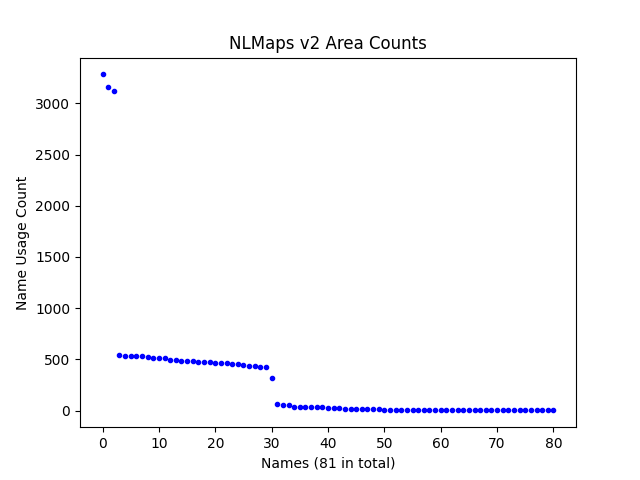
\includegraphics[width=\textwidth]{fig/nlmaps_v2_area_counts.png}
  \caption[Area names in \nlmapstwo{}]{Area names in \nlmapstwo{}.}
  \label{fig:nlmaps-v2-areas}
\end{figure}

Some imbalance is also present in the values of \osmtag{name=*} tags in the
\mrl{nwr} operators, which are mostly names of points of interests. However, the
imbalance is much less pronounced in this case and with \num{5969} different
names there is a large variety of different names. This is illustrated in
Figure~\ref{fig:nlmaps-v2-nwrs}.

\begin{figure}[h]
  \centering
  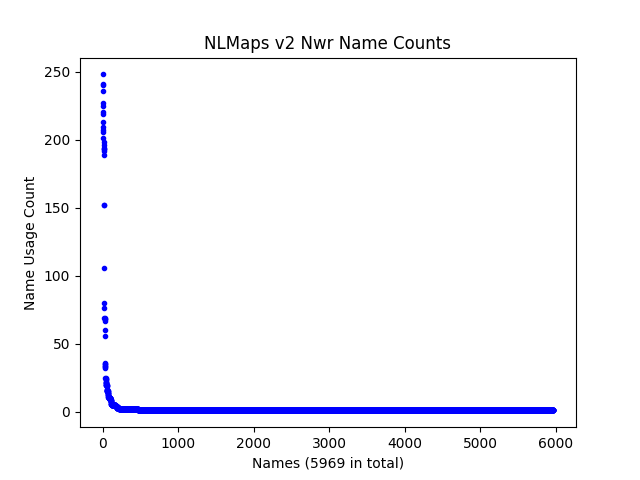
\includegraphics[width=\textwidth]{fig/nlmaps_v2_nwr_name_counts.png}
  \caption[Nwr names in \nlmapstwo{}]{Nwr names in \nlmapstwo{}.}
  \label{fig:nlmaps-v2-nwrs}
\end{figure}

This lack of variety is not a problem when training on the masked data and using
an external NER system because the model will only ever see the placeholders for
the location names. However, models directly trained on \nlmapstwo{} will learn
a strong bias with respect to location names, as evidenced by the model
hallucinating the area \emph{Paris} out of thin air as seen in
Figure~\ref{fig:valleys-around-zenica}. An improved version of the dataset
should provide a large variety of names, which should also stem from a variety
of different countries and languages.

\subsection{Unnatural Wording of Queries}
\label{sec:unnatural-wording}

It is some queries’ purpose to extract the value associated with a certain key
from the result set, which is reflected in the MRL by operations like
\mrl{findkey('name')} or \mrl{findkey('opening_hours)} inside the \mrl{qtype}
clause. This intention can be coded in the NL query through wordings like
\nl{What are the names …?}, \nl{Name all the …!}, \nl{Tell me the
  opening hours …!} or \nl{When is … open?}.

This type of NL query is of course present in \nlmapstwo{}, but there are also
queries which are simply prefixed by an OSM key, which is then understood as an
indication to extract that key via the the \mrl{findkey} operator. Five such
queries are shown in Figure~\ref{fig:nlmaps-v2-unnatural-wording}. Some of them
(such as \nl{name Paris buy ice cream}) can pass as crude wordings of legitimate
queries.

\begin{figure}[h]
  \centering
  \begin{lstlisting}[style=MyNL]
wheelchair Jewelry Shops near München in walking distance
amenity closest Gas Station from Düsseldorf
bicycle Cycle Paths in Sheffield
source Sports Centres near Blakenhale Road in Birmingham
name Paris buy ice cream
  \end{lstlisting}
  \caption[Unnatural \nlmapstwo{} queries]{NL queries from \nlmapstwo{} where
    the OSM key that is to be extracted is just added as a prefix.}
  \label{fig:nlmaps-v2-unnatural-wording}
\end{figure}

Others are misleading or at least ambiguous. E.g., \nl{wheelchair Jewelry Shops
  near München in walking distance} is understood as being equivalent to
\nl{Tell me if the Jewelry Shops near München are wheelchair-accessible.},
whereas it could just as well mean \nl{Which Jewelry Shops near München are
  wheelchair-accessible?}, which might even be the more likely query.

Some are actually nonsensical: Gas stations are selected via
\osmtag{amenity=fuel} in the first place, so the \osmtag{amenity} value will of
course always be \osmtag{fuel}; similarly for the bicycle path example. And some
keys are rarely worth asking for because they are in general not interesting,
such as the \osmtag{source} key, which is used by OSM mappers to give the
information source used for mapping an object (e.g.\ aerial photography or survey
in person).

Paired with the lack of linguistic variety, this method of unnaturally prefixing
an otherwise complete NL query with an OSM key is actually harmful when queries
are encountered that start with unseen phrases. This is evidenced by the query
\nl{Show me the cafes near Martinskirche in Westheim} in
Figure~\ref{fig:cafes-near-martinskirche}, where the model attempts to extract
the value of a nonsensical \osmtag{show:me} key.

With the exception of somewhat reasonable cases like prefixing \nl{name}, all of
these queries should be deleted from the dataset in order to improve it.

\subsection{Improper Usage of OSM Tags}
\label{sec:improper-osm-tags}

So far we have only discussed intrinsic qualities of \nlmapstwo{} by examining
NL and MRL queries and their consistency without paying heed to the usage of the
covered tags in the OSM database. This is of course important because the tags
only derive their meaning from their usage in the dataset. While most tags are
used correctly in \nlmapstwo{} (e.g.\ \osmtag{shop=clothes} used in MRLs for
queries asking for \nl{clothing stores}), there are also some tags that are not
in current use in OSM, have never been in use or their use differs from what
they are understood to mean in \nlmapstwo{}. Most of these errors are inherited
from the table discussed in Section~\ref{sec:term-tag-inconsistencies}. Some
examples are given:

\begin{itemize}
\item
  \osmtag{amenity=park}\footnote{\url{https://wiki.openstreetmap.org/wiki/Tag:amenity=park}.}
  is sometimes used in \nlmapstwo{}, even though \osmtag{leisure=park} is the
  proper tag for parks. As of April 2021, \osmtag{amenity=park} is used only
  \num{30} times in OSM.
\item \osmtag{place=house} has probably never had any usage in OSM, even though
  it is used in \nlmapstwo{}.
\item Churches\footnote{\url{https://wiki.openstreetmap.org/wiki/Church}.} are
  places of Christian worship and can be identified by the tag combination
  \osmtag{amenity=place_of_worship + religion=christian}. However, \nlmapstwo{}
  uses \osmtag{building=church} (and also \osmtag{historic=church}), which
  should be used for buildings \emph{built as} churches. They may be used for
  another purpose now\footnote{The Hagia Sophia mosque in Istanbul may be the
    most famous example of this.}, while some non-church buildings may be used
  for holding church services and are thus churches.\footnote{The analogous
    situation of a non-religious building being used as a mosque is very common
    in Germany, for example.}
\end{itemize}

Choosing the correct tag or tag combination is virtually irrelevant for training
the machine learning model, but it will obviously be essential when the MRLs are
actually used for an OSM lookup. Finer points of this multifaceted issue will be
discussed at a later point in this thesis.

\section{Improving on \nlmapstwo{}}

The most obvious way to produce a dataset that is closer to real world queries
is to source it from actual users via an annotation project. This is what will
be described later in this thesis. But in order to collect data efficiently, a
model is helpful that answers the simple questions correctly already, so that
annotators will spend less time constructing trivial MRLs. And even for more
difficult queries, it’s easier to adjust an MRL that is only slightly incorrect
than one with several errors.

Therefore, it is reasonable to make an effort of improving on the existing
\nlmapstwo{} dataset by fixing some of its shortcomings and by extending it with
new queries generated by an improved templating approach. These steps are
described in the following two sections.

\subsection{Fixing \nlmapstwo{} Shortcomings}

The fixing of shortcomings in the existing dataset concentrates on making it
more consistent. For reproducibility, all of the fixes are made in a
script,\footnote{\url{https://gitlab.cl.uni-heidelberg.de/will/nlmaps-tools/-/blob/handed_in/nlmaps_tools/fix_nlmaps_v2.py}.},
which does the following:

\begin{itemize}
\item OSM tags in the MRLs are replaced by non-deprecated counterparts or by the
  union of all applicable tags, in some cases depending on the content of the NL
  query. Cf.\ Sections~\ref{sec:term-tag-inconsistencies} and
  \ref{sec:improper-osm-tags}. Examples:
  \begin{itemize}
  \item \osmtag{amenity=park} \textrightarrow{} \osmtag{leisure=park}
  \item \osmtag{landuse=forest} \textrightarrow{} \mrl{or(landuse=forest,
      natural=wood)}
  \item NL asks for bars and MRL contains \osmtag{amenity=pub} \textrightarrow{}
    \osmtag{amenity=bar}
  \end{itemize}

\item The operator \mrl{area} in a \mrl{center} clause without an \mrl{nwr}
  operator is replaced by the \mrl{nwr} operator.
  Cf.\ Section~\ref{sec:mrl-inconsistencies}.

\item NL-MRL pairs where an OSM tag was used as the prefix of the NL query to
  indicate a matching \mrl{findkey} operator are removed with the exception of
  the keys \osmtag{name}, \osmtag{opening_hours} and \osmtag{website}.
  Cf.\ Section~\ref{sec:unnatural-wording}.
\end{itemize}

By applying these changes to \nlmapstwo{}, \num{2168} MRLs are modified and a
further \num{1859} instances are deleted resulting in a modified dataset
containing \num{26750} NL-MRL pairs, which will be called \nlmapstwoone{}. More
detailed numbers are given in Table~\ref{tab:nlmaps-v2.1-stats}. Note that the
NL side of queries is never modified in the process.

\begin{table}
  \centering
  \begin{tabular}{lrrrr}
    \toprule
    Split & \nlmapstwo{} & Modified & Deleted & \nlmapstwoone{}\\
    \midrule
    Train & \num{16172} & \num{1236} & \num{1059} & \num{15113}\\
    Dev & \num{1843} & \num{136} & \num{109} & \num{1734}\\
    Test & \num{10594} & \num{796} & \num{691} & \num{9903}\\
    \midrule
    Total & \num{28609} & \num{2168} & \num{1859} & \num{26750}\\
    \bottomrule
  \end{tabular}
  \caption[\nlmapstwoone{} statistics]{Numbers of deletions and modifications
    going from \nlmapstwo{} to \nlmapstwoone{}.}
  \label{tab:nlmaps-v2.1-stats}
\end{table}

\subsection{Extension of \nlmapstwo{}}

In order to address also the other shortcomings, a new dataset is generated in a
more sophisticated templating approach. The new approach differs by the one used
for \nlmapstwo{} in the following ways:

\begin{itemize}
\item More templates are used.
\item There is significant variation within each template.
\item More area names are used.
\item Area names are more evenly distributed.
\item More OSM tags are used. For this, the information from the table used for
  \nlmapstwo{} is manually extended.
\item Errors in the tag usage (as discussed in
  Sections~\ref{sec:term-tag-inconsistencies} and \ref{sec:improper-osm-tags})
  are of course avoided in the first place.
\end{itemize}

\begin{figure}[h]
  \centering
  \begin{lstlisting}[style=MyJinja]
when
{{ choose(['can I', 'can we', 'to'], [0.3, 0.3, 0.4]) }}
{{ choose(['visit', 'go to'], [0.6, 0.4]) }}

  {{ choose(['the', 'all', 'all the', ''], [0.2, 0.2, 0.2, 0.4]) }}

  {{ choose(['a', 'some', 'any', '']) }}

{{ thing_plural if plural else thing_singular }}

{{ optional('?') }}
  \end{lstlisting}
  \caption[Opening hours template]{Simple template for one version of queries
    for opening hours.}
  \label{fig:opening-hours-template}
\end{figure}

The templates are designed to be probabilistic. I.e., instead of being rigid,
they are essentially decision trees with various decisions being made to arrive
at the final wording of an NL query. Figure~\ref{fig:opening-hours-template}
shows one of several templates used for generating queries that ask for opening
hours. By choosing phrases according to the given probability distributions, it
can produce queries like \nl{when to visit theatres in Bratislava?} or \nl{when
  can I go to a cinema in Hannover}. The resulting dataet is called
\nlmapsthreea{}.

The location names are collected via extracting all areas and named places from
different regions in countries that use variations of the Latin alphabet. This
is done to ensure that location names from various languages are included in the
dataset.\footnote{When generating a query for things around some named place
  inside an area, both the place and the area are randomly selected
  independently from each other. This leads to queries like \nl{restaurants near
    Eiffel Tower in Rome}, which do not make sense in practice because there is
  no Eiffel Tower in Rome, but that doesn’t matter since the model is just
  supposed to learn to copy the names to the appropriate place in the MRL.}
Figure~\ref{fig:nlmaps-v3a-areas} shows a large variety in
well-distributed area names. This is in contrast with the situation in
\nlmapstwo{} shown in Figure~\ref{fig:nlmaps-v2-areas}.

\begin{figure}[h]
  \centering
  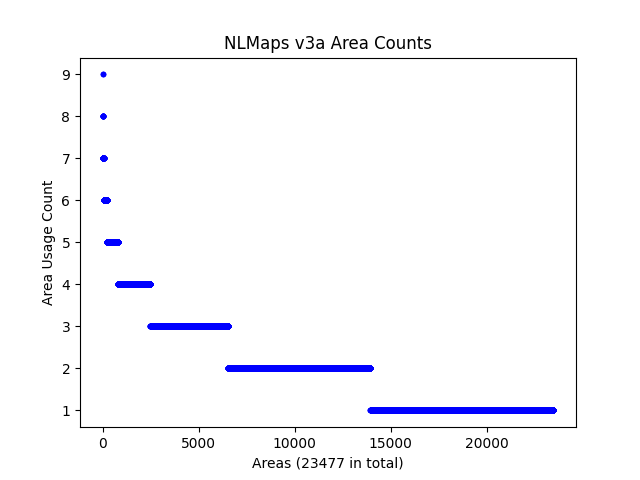
\includegraphics[width=\textwidth]{fig/nlmaps_v3a_area_counts.png}
  \caption[Area names in \nlmapsthreea{}]{Area values in \nlmapsthreea{}.}
  \label{fig:nlmaps-v3a-areas}
\end{figure}

In order to train models that are robust against typing errors and other small
spelling deviations, some noise is added to the NL queries in
\nlmapsthreea{} by switching a character for another with a chance of
\SI{1}{\%}. Names of locations are never touched, however. The resulting dataset
with noise is called \nlmapsthreeb{} and a random sample of NL queries is
shown in Figure~\ref{fig:nlmaps-v3b-sample}.

\begin{figure}[h]
  \centering
\begin{lstlisting}[style=MyNL]
what bathrooms in Záluží are around Zur Stöpe?
what preschools in Sadek are in walking distance hrom Gasthaus Tannengarten?
Do some veterinary surgerils exist east of studna in Montgeron (canton de Draveil)
Gire me any department store around ROBOT in Neue Vahr Südost
which setvice rosd in Bardzice is south of Le Ciré Jaune?
show me the opening times of all the monorail in the area of The KPH in Świecie
Which viewpoint is there in Miño de San Esteban?
In Grabowiec, what are the opening hours of all the boatyards less than 80 kilometres away from MakroMueble
Indicate the coordinaSes of all byways Tn přírodní památka Branžovy.
Are there parks east of Tigery?
\end{lstlisting}
  \caption[10 random \nlmapsthreeb{} queries]{10 random \nlmapsthreeb{} queries.}
  \label{fig:nlmaps-v3b-sample}
\end{figure}

Finally, we concatenate \nlmapstwo{} and \nlmapsthreeb{} and call the result
\nlmapsthree{}. Since we generate exactly as many instances for
\nlmapsthreeb{} as are present in the corresponding split of \nlmapstwoone{},
\nlmapsthree{} is exactly twice as large as \nlmapstwoone{}.

The linguistic diversity of the resulting datasets is quantified by the entropy
rate estimated by the conditional entropy on trigrams, as described in
Section~\ref{sec:little-linguistic-diversity}. Table \ref{tab:v2-v3-overview}
offers an overview over the datasets.

\begin{table}[h]
  \centering
  \begin{tabular}{lrrrrr}
    \toprule
    Measure & \nlmtwo{} & \nlmtwoone{} & \nlmthreea{} & \nlmthreeb{} & \nlmthree{}\\
    \midrule
    Instances & \num{28609} & \num{26750} & \num{53500} & \num{53500} & \num{53500}\\
    Conditional Entropy & \num{2.11} & \num{2.08} & \num{2.85} & \num{2.93} & \num{2.73}\\
    Avg. Tokens per NL & \num{6.98} & \num{7.02} & \num{10.72} & \num{10.69} & \num{8.85}\\
    \bottomrule
  \end{tabular}
  \caption[Dataset statistics]{Comparison of dataset statistics. Entropy rates
    are estimated by the conditional entropy trigrams.}
  \label{tab:v2-v3-overview}
\end{table}

%%% Local Variables:
%%% coding: utf-8
%%% mode: latex
%%% TeX-engine: xetex
%%% TeX-parse-self: t
%%% TeX-command-extra-options: "-shell-escape"
%%% TeX-master: "../thesis"
%%% End:

%\include{tex/Web Interface}

%\chapter{Experiments}
\label{ch:experiments}

Our goal is simulating different strategies of online learning for the new web
interface. Before we can do that, we first pre-train parsers in
Section~\ref{sec:pre-training} on the existing datasets \nlmapstwo{} and the
variations we introduced in \nlmapsthree{} and evaluate whether the dataset
extensions yield any improvement in parser quality. In
Section~\ref{sec:annotation}, we then hire annotators to use our web interface
to ask NL queries and correct the MRL parse if it is incorrect, thus collecting
a new dataset consisting of real user queries. Finally, in
Section~\ref{sec:online-simulation} we use the newly acquired dataset for
evaluating various online learning setups.

For all our experiments, we use the same model architecture: A character-based
one-layer bidirectional GRU encoder-decoder \parencite{cho-2014} model with
attention.\parencite{bahdanau-2015} The dimension of both source and target
embeddings is 620, the encoder layer size is 500, the decoder layer size is 1000
and we don’t use dropout. This model configuration is adopted from
\textcite{staniek-2020}.

\section{Training on \nlmapstwo{} and \nlmapsthree{}}
\label{sec:pre-training}

While \textcite{staniek-2020} trained his model on the \nlmapstwo{} dataset for
100 epochs (of 16172 instances each), we train our models in this section for a
shorter time, which is still enough for sufficient convergence: The model on
\nlmapstwoone{} is trained for 60 epochs (of 15113 instances each), while the
models on variations of \nlmapsthree{} are trained for 30 epochs (of 30226
instances each). All models are trained with the Adam optimizer (\(\beta_1 =
0.9\) and \(\beta_2 = 0.999\)) and a learning rate of \num{0.0002}

Table~\ref{tab:pre-trained-performance} shows the results of testing the models
on the different variations of \nlmaps{} datasets. Recall: \nlmtwoone{} is the
result of fixing issues in the MRL queries of \nlmtwo{}, but has identical NL
queries; \nlmthreea{} is purely generated with probabilistic templates and
\nlmthreeb{} is its counterpart with added noise; \nlmthreenormal{} is
\nlmtwoone{} + \nlmthreea{} and \nlmthree{} is \nlmtwoone{} + \nlmthreeb{}. The
datasets \nlmfourraw{} and \nlmfour{} are introduced in
Section~\ref{sec:annotation} and are the user-supplied MRL-NL pairs with some
corrections applied to them in \nlmfour{}. Even though the last two datasets
were not yet available when the models were pre-trained, we still evaluate the
pre-trained models on them in this section because we consider the results on
these user-supplied queries the most relevant.

\begin{table}[h]
  \centering
  \begin{tabular}{lcccccccc}
    \toprule
    \diagbox{Train}{Test} & \nlmtwo{} & \nlmtwoone{} & \nlmthreea{} & \nlmthreeb{} & \nlmthreenormal{} & \nlmthree{} & \nlmfourraw{} & \nlmfour{}\\
    \midrule
    \textcite{staniek-2020} & \bfnum{0.898} & \num{0.844} & \num{0.039} & \num{0.033} & \num{0.441} & \num{0.439} & \num{0.050} & \num{0.052}\\
    \nlmtwoone{} & \num{0.783} & \num{0.913} & \num{0.034} & \num{0.029} & \num{0.474} & \num{0.471} & \num{0.070} & \num{0.069}\\
    \nlmthreea{} & \num{0.224} & \num{0.251} & \bfnum{0.987} & \num{0.789} & \num{0.618} & \num{0.519} & \num{0.217} & \num{0.223}\\
    \nlmthreeb{} & \num{0.372} & \num{0.424} & \num{0.976} & \bfnum{0.884} & \num{0.700} & \num{0.656} & \num{0.226} & \num{0.233}\\
    \nlmthreenormal{} & \num{0.790} & \bfnum{0.919} & \num{0.978} & \num{0.792} & \bfnum{0.948} & \num{0.857} & \bfnum{0.307} & \bfnum{0.311}\\
    \nlmthree{} & \num{0.787} & \num{0.913} & \num{0.950} & \num{0.834} & \num{0.931} & \bfnum{0.874} & \num{0.281} & \num{0.289}\\
    \bottomrule
  \end{tabular}
  \caption{Performance of pre-trained parsers}
  \label{tab:pre-trained-performance}
\end{table}

Unsurprisingly, the model by \textcite{staniek-2020}, which was trained on
\nlmapstwo{}, performs best on the corresponding test set with an accuracy of
\SI{89.8}{\%}. The model trained on \nlmtwoone{}, which contains the fixes of
tag usage and inconsistencies described in Chapter~\ref{ch:nlmaps-improvement},
achieves a higher accuracy on its corresponding test set with \SI{91.3}{\%}.
This is to be expected since the resolution of inconsistencies in MRL structure
and tag usage makes a new part of the dataset accessible for confident
predictions in the first place. These two models’ performance drops dramatically
on new datasets. An error analysis (see Figure~\ref{fig:v21-errors}) shows that
not only does the model trained on \nlmtwoone{} make an error in the
\mrl{target_nwr} operator in over \SI{70}{\%} of queries from the \nlmapsfour{}
test set, the recognized \mrl{area} is false in more than half the queries, as
well.

\begin{figure}[h]
  \centering
  \resizebox{\textwidth}{!}{%% Creator: Matplotlib, PGF backend
%%
%% To include the figure in your LaTeX document, write
%%   \input{<filename>.pgf}
%%
%% Make sure the required packages are loaded in your preamble
%%   \usepackage{pgf}
%%
%% and, on pdftex
%%   \usepackage[utf8]{inputenc}\DeclareUnicodeCharacter{2212}{-}
%%
%% or, on luatex and xetex
%%   \usepackage{unicode-math}
%%
%% Figures using additional raster images can only be included by \input if
%% they are in the same directory as the main LaTeX file. For loading figures
%% from other directories you can use the `import` package
%%   \usepackage{import}
%%
%% and then include the figures with
%%   \import{<path to file>}{<filename>.pgf}
%%
%% Matplotlib used the following preamble
%%   \usepackage{fontspec}
%%   \setmainfont{LinLibertine_R.otf}[Path=/usr/share/texmf-dist/fonts/opentype/public/libertine/]
%%   \setsansfont{LinLibertine_R.otf}[Path=/usr/share/texmf-dist/fonts/opentype/public/libertine/]
%%   \setmonofont{DejaVuSansMono.ttf}[Path=/home/gorgor/.virtualenvs/ma/lib/python3.9/site-packages/matplotlib/mpl-data/fonts/ttf/]
%%
\begingroup%
\makeatletter%
\begin{pgfpicture}%
\pgfpathrectangle{\pgfpointorigin}{\pgfqpoint{6.400000in}{3.500000in}}%
\pgfusepath{use as bounding box, clip}%
\begin{pgfscope}%
\pgfsetbuttcap%
\pgfsetmiterjoin%
\definecolor{currentfill}{rgb}{1.000000,1.000000,1.000000}%
\pgfsetfillcolor{currentfill}%
\pgfsetlinewidth{0.000000pt}%
\definecolor{currentstroke}{rgb}{1.000000,1.000000,1.000000}%
\pgfsetstrokecolor{currentstroke}%
\pgfsetdash{}{0pt}%
\pgfpathmoveto{\pgfqpoint{0.000000in}{0.000000in}}%
\pgfpathlineto{\pgfqpoint{6.400000in}{0.000000in}}%
\pgfpathlineto{\pgfqpoint{6.400000in}{3.500000in}}%
\pgfpathlineto{\pgfqpoint{0.000000in}{3.500000in}}%
\pgfpathclose%
\pgfusepath{fill}%
\end{pgfscope}%
\begin{pgfscope}%
\pgfsetbuttcap%
\pgfsetmiterjoin%
\definecolor{currentfill}{rgb}{1.000000,1.000000,1.000000}%
\pgfsetfillcolor{currentfill}%
\pgfsetlinewidth{0.000000pt}%
\definecolor{currentstroke}{rgb}{0.000000,0.000000,0.000000}%
\pgfsetstrokecolor{currentstroke}%
\pgfsetstrokeopacity{0.000000}%
\pgfsetdash{}{0pt}%
\pgfpathmoveto{\pgfqpoint{1.024000in}{0.490000in}}%
\pgfpathlineto{\pgfqpoint{6.272000in}{0.490000in}}%
\pgfpathlineto{\pgfqpoint{6.272000in}{3.430000in}}%
\pgfpathlineto{\pgfqpoint{1.024000in}{3.430000in}}%
\pgfpathclose%
\pgfusepath{fill}%
\end{pgfscope}%
\begin{pgfscope}%
\pgfpathrectangle{\pgfqpoint{1.024000in}{0.490000in}}{\pgfqpoint{5.248000in}{2.940000in}}%
\pgfusepath{clip}%
\pgfsetbuttcap%
\pgfsetmiterjoin%
\definecolor{currentfill}{rgb}{1.000000,0.000000,0.000000}%
\pgfsetfillcolor{currentfill}%
\pgfsetlinewidth{0.000000pt}%
\definecolor{currentstroke}{rgb}{0.000000,0.000000,0.000000}%
\pgfsetstrokecolor{currentstroke}%
\pgfsetstrokeopacity{0.000000}%
\pgfsetdash{}{0pt}%
\pgfpathmoveto{\pgfqpoint{1.024000in}{0.623636in}}%
\pgfpathlineto{\pgfqpoint{1.997139in}{0.623636in}}%
\pgfpathlineto{\pgfqpoint{1.997139in}{0.829231in}}%
\pgfpathlineto{\pgfqpoint{1.024000in}{0.829231in}}%
\pgfpathclose%
\pgfusepath{fill}%
\end{pgfscope}%
\begin{pgfscope}%
\pgfpathrectangle{\pgfqpoint{1.024000in}{0.490000in}}{\pgfqpoint{5.248000in}{2.940000in}}%
\pgfusepath{clip}%
\pgfsetbuttcap%
\pgfsetmiterjoin%
\definecolor{currentfill}{rgb}{1.000000,0.000000,0.000000}%
\pgfsetfillcolor{currentfill}%
\pgfsetlinewidth{0.000000pt}%
\definecolor{currentstroke}{rgb}{0.000000,0.000000,0.000000}%
\pgfsetstrokecolor{currentstroke}%
\pgfsetstrokeopacity{0.000000}%
\pgfsetdash{}{0pt}%
\pgfpathmoveto{\pgfqpoint{1.024000in}{1.034825in}}%
\pgfpathlineto{\pgfqpoint{1.322893in}{1.034825in}}%
\pgfpathlineto{\pgfqpoint{1.322893in}{1.240420in}}%
\pgfpathlineto{\pgfqpoint{1.024000in}{1.240420in}}%
\pgfpathclose%
\pgfusepath{fill}%
\end{pgfscope}%
\begin{pgfscope}%
\pgfpathrectangle{\pgfqpoint{1.024000in}{0.490000in}}{\pgfqpoint{5.248000in}{2.940000in}}%
\pgfusepath{clip}%
\pgfsetbuttcap%
\pgfsetmiterjoin%
\definecolor{currentfill}{rgb}{1.000000,0.000000,0.000000}%
\pgfsetfillcolor{currentfill}%
\pgfsetlinewidth{0.000000pt}%
\definecolor{currentstroke}{rgb}{0.000000,0.000000,0.000000}%
\pgfsetstrokecolor{currentstroke}%
\pgfsetstrokeopacity{0.000000}%
\pgfsetdash{}{0pt}%
\pgfpathmoveto{\pgfqpoint{1.024000in}{1.446014in}}%
\pgfpathlineto{\pgfqpoint{1.128265in}{1.446014in}}%
\pgfpathlineto{\pgfqpoint{1.128265in}{1.651608in}}%
\pgfpathlineto{\pgfqpoint{1.024000in}{1.651608in}}%
\pgfpathclose%
\pgfusepath{fill}%
\end{pgfscope}%
\begin{pgfscope}%
\pgfpathrectangle{\pgfqpoint{1.024000in}{0.490000in}}{\pgfqpoint{5.248000in}{2.940000in}}%
\pgfusepath{clip}%
\pgfsetbuttcap%
\pgfsetmiterjoin%
\definecolor{currentfill}{rgb}{1.000000,0.000000,0.000000}%
\pgfsetfillcolor{currentfill}%
\pgfsetlinewidth{0.000000pt}%
\definecolor{currentstroke}{rgb}{0.000000,0.000000,0.000000}%
\pgfsetstrokecolor{currentstroke}%
\pgfsetstrokeopacity{0.000000}%
\pgfsetdash{}{0pt}%
\pgfpathmoveto{\pgfqpoint{1.024000in}{1.857203in}}%
\pgfpathlineto{\pgfqpoint{4.833144in}{1.857203in}}%
\pgfpathlineto{\pgfqpoint{4.833144in}{2.062797in}}%
\pgfpathlineto{\pgfqpoint{1.024000in}{2.062797in}}%
\pgfpathclose%
\pgfusepath{fill}%
\end{pgfscope}%
\begin{pgfscope}%
\pgfpathrectangle{\pgfqpoint{1.024000in}{0.490000in}}{\pgfqpoint{5.248000in}{2.940000in}}%
\pgfusepath{clip}%
\pgfsetbuttcap%
\pgfsetmiterjoin%
\definecolor{currentfill}{rgb}{1.000000,0.000000,0.000000}%
\pgfsetfillcolor{currentfill}%
\pgfsetlinewidth{0.000000pt}%
\definecolor{currentstroke}{rgb}{0.000000,0.000000,0.000000}%
\pgfsetstrokecolor{currentstroke}%
\pgfsetstrokeopacity{0.000000}%
\pgfsetdash{}{0pt}%
\pgfpathmoveto{\pgfqpoint{1.024000in}{2.268392in}}%
\pgfpathlineto{\pgfqpoint{1.510570in}{2.268392in}}%
\pgfpathlineto{\pgfqpoint{1.510570in}{2.473986in}}%
\pgfpathlineto{\pgfqpoint{1.024000in}{2.473986in}}%
\pgfpathclose%
\pgfusepath{fill}%
\end{pgfscope}%
\begin{pgfscope}%
\pgfpathrectangle{\pgfqpoint{1.024000in}{0.490000in}}{\pgfqpoint{5.248000in}{2.940000in}}%
\pgfusepath{clip}%
\pgfsetbuttcap%
\pgfsetmiterjoin%
\definecolor{currentfill}{rgb}{1.000000,0.000000,0.000000}%
\pgfsetfillcolor{currentfill}%
\pgfsetlinewidth{0.000000pt}%
\definecolor{currentstroke}{rgb}{0.000000,0.000000,0.000000}%
\pgfsetstrokecolor{currentstroke}%
\pgfsetstrokeopacity{0.000000}%
\pgfsetdash{}{0pt}%
\pgfpathmoveto{\pgfqpoint{1.024000in}{2.679580in}}%
\pgfpathlineto{\pgfqpoint{3.790495in}{2.679580in}}%
\pgfpathlineto{\pgfqpoint{3.790495in}{2.885175in}}%
\pgfpathlineto{\pgfqpoint{1.024000in}{2.885175in}}%
\pgfpathclose%
\pgfusepath{fill}%
\end{pgfscope}%
\begin{pgfscope}%
\pgfpathrectangle{\pgfqpoint{1.024000in}{0.490000in}}{\pgfqpoint{5.248000in}{2.940000in}}%
\pgfusepath{clip}%
\pgfsetbuttcap%
\pgfsetmiterjoin%
\definecolor{currentfill}{rgb}{1.000000,0.000000,0.000000}%
\pgfsetfillcolor{currentfill}%
\pgfsetlinewidth{0.000000pt}%
\definecolor{currentstroke}{rgb}{0.000000,0.000000,0.000000}%
\pgfsetstrokecolor{currentstroke}%
\pgfsetstrokeopacity{0.000000}%
\pgfsetdash{}{0pt}%
\pgfpathmoveto{\pgfqpoint{1.024000in}{3.090769in}}%
\pgfpathlineto{\pgfqpoint{1.872021in}{3.090769in}}%
\pgfpathlineto{\pgfqpoint{1.872021in}{3.296364in}}%
\pgfpathlineto{\pgfqpoint{1.024000in}{3.296364in}}%
\pgfpathclose%
\pgfusepath{fill}%
\end{pgfscope}%
\begin{pgfscope}%
\pgfpathrectangle{\pgfqpoint{1.024000in}{0.490000in}}{\pgfqpoint{5.248000in}{2.940000in}}%
\pgfusepath{clip}%
\pgfsetbuttcap%
\pgfsetmiterjoin%
\definecolor{currentfill}{rgb}{0.756863,0.988235,0.756863}%
\pgfsetfillcolor{currentfill}%
\pgfsetlinewidth{0.000000pt}%
\definecolor{currentstroke}{rgb}{0.000000,0.000000,0.000000}%
\pgfsetstrokecolor{currentstroke}%
\pgfsetstrokeopacity{0.000000}%
\pgfsetdash{}{0pt}%
\pgfpathmoveto{\pgfqpoint{1.997139in}{0.623636in}}%
\pgfpathlineto{\pgfqpoint{6.272000in}{0.623636in}}%
\pgfpathlineto{\pgfqpoint{6.272000in}{0.829231in}}%
\pgfpathlineto{\pgfqpoint{1.997139in}{0.829231in}}%
\pgfpathclose%
\pgfusepath{fill}%
\end{pgfscope}%
\begin{pgfscope}%
\pgfpathrectangle{\pgfqpoint{1.024000in}{0.490000in}}{\pgfqpoint{5.248000in}{2.940000in}}%
\pgfusepath{clip}%
\pgfsetbuttcap%
\pgfsetmiterjoin%
\definecolor{currentfill}{rgb}{0.756863,0.988235,0.756863}%
\pgfsetfillcolor{currentfill}%
\pgfsetlinewidth{0.000000pt}%
\definecolor{currentstroke}{rgb}{0.000000,0.000000,0.000000}%
\pgfsetstrokecolor{currentstroke}%
\pgfsetstrokeopacity{0.000000}%
\pgfsetdash{}{0pt}%
\pgfpathmoveto{\pgfqpoint{1.322893in}{1.034825in}}%
\pgfpathlineto{\pgfqpoint{6.272000in}{1.034825in}}%
\pgfpathlineto{\pgfqpoint{6.272000in}{1.240420in}}%
\pgfpathlineto{\pgfqpoint{1.322893in}{1.240420in}}%
\pgfpathclose%
\pgfusepath{fill}%
\end{pgfscope}%
\begin{pgfscope}%
\pgfpathrectangle{\pgfqpoint{1.024000in}{0.490000in}}{\pgfqpoint{5.248000in}{2.940000in}}%
\pgfusepath{clip}%
\pgfsetbuttcap%
\pgfsetmiterjoin%
\definecolor{currentfill}{rgb}{0.756863,0.988235,0.756863}%
\pgfsetfillcolor{currentfill}%
\pgfsetlinewidth{0.000000pt}%
\definecolor{currentstroke}{rgb}{0.000000,0.000000,0.000000}%
\pgfsetstrokecolor{currentstroke}%
\pgfsetstrokeopacity{0.000000}%
\pgfsetdash{}{0pt}%
\pgfpathmoveto{\pgfqpoint{1.128265in}{1.446014in}}%
\pgfpathlineto{\pgfqpoint{6.272000in}{1.446014in}}%
\pgfpathlineto{\pgfqpoint{6.272000in}{1.651608in}}%
\pgfpathlineto{\pgfqpoint{1.128265in}{1.651608in}}%
\pgfpathclose%
\pgfusepath{fill}%
\end{pgfscope}%
\begin{pgfscope}%
\pgfpathrectangle{\pgfqpoint{1.024000in}{0.490000in}}{\pgfqpoint{5.248000in}{2.940000in}}%
\pgfusepath{clip}%
\pgfsetbuttcap%
\pgfsetmiterjoin%
\definecolor{currentfill}{rgb}{0.756863,0.988235,0.756863}%
\pgfsetfillcolor{currentfill}%
\pgfsetlinewidth{0.000000pt}%
\definecolor{currentstroke}{rgb}{0.000000,0.000000,0.000000}%
\pgfsetstrokecolor{currentstroke}%
\pgfsetstrokeopacity{0.000000}%
\pgfsetdash{}{0pt}%
\pgfpathmoveto{\pgfqpoint{4.833144in}{1.857203in}}%
\pgfpathlineto{\pgfqpoint{6.272000in}{1.857203in}}%
\pgfpathlineto{\pgfqpoint{6.272000in}{2.062797in}}%
\pgfpathlineto{\pgfqpoint{4.833144in}{2.062797in}}%
\pgfpathclose%
\pgfusepath{fill}%
\end{pgfscope}%
\begin{pgfscope}%
\pgfpathrectangle{\pgfqpoint{1.024000in}{0.490000in}}{\pgfqpoint{5.248000in}{2.940000in}}%
\pgfusepath{clip}%
\pgfsetbuttcap%
\pgfsetmiterjoin%
\definecolor{currentfill}{rgb}{0.756863,0.988235,0.756863}%
\pgfsetfillcolor{currentfill}%
\pgfsetlinewidth{0.000000pt}%
\definecolor{currentstroke}{rgb}{0.000000,0.000000,0.000000}%
\pgfsetstrokecolor{currentstroke}%
\pgfsetstrokeopacity{0.000000}%
\pgfsetdash{}{0pt}%
\pgfpathmoveto{\pgfqpoint{1.510570in}{2.268392in}}%
\pgfpathlineto{\pgfqpoint{6.272000in}{2.268392in}}%
\pgfpathlineto{\pgfqpoint{6.272000in}{2.473986in}}%
\pgfpathlineto{\pgfqpoint{1.510570in}{2.473986in}}%
\pgfpathclose%
\pgfusepath{fill}%
\end{pgfscope}%
\begin{pgfscope}%
\pgfpathrectangle{\pgfqpoint{1.024000in}{0.490000in}}{\pgfqpoint{5.248000in}{2.940000in}}%
\pgfusepath{clip}%
\pgfsetbuttcap%
\pgfsetmiterjoin%
\definecolor{currentfill}{rgb}{0.756863,0.988235,0.756863}%
\pgfsetfillcolor{currentfill}%
\pgfsetlinewidth{0.000000pt}%
\definecolor{currentstroke}{rgb}{0.000000,0.000000,0.000000}%
\pgfsetstrokecolor{currentstroke}%
\pgfsetstrokeopacity{0.000000}%
\pgfsetdash{}{0pt}%
\pgfpathmoveto{\pgfqpoint{3.790495in}{2.679580in}}%
\pgfpathlineto{\pgfqpoint{6.272000in}{2.679580in}}%
\pgfpathlineto{\pgfqpoint{6.272000in}{2.885175in}}%
\pgfpathlineto{\pgfqpoint{3.790495in}{2.885175in}}%
\pgfpathclose%
\pgfusepath{fill}%
\end{pgfscope}%
\begin{pgfscope}%
\pgfpathrectangle{\pgfqpoint{1.024000in}{0.490000in}}{\pgfqpoint{5.248000in}{2.940000in}}%
\pgfusepath{clip}%
\pgfsetbuttcap%
\pgfsetmiterjoin%
\definecolor{currentfill}{rgb}{0.756863,0.988235,0.756863}%
\pgfsetfillcolor{currentfill}%
\pgfsetlinewidth{0.000000pt}%
\definecolor{currentstroke}{rgb}{0.000000,0.000000,0.000000}%
\pgfsetstrokecolor{currentstroke}%
\pgfsetstrokeopacity{0.000000}%
\pgfsetdash{}{0pt}%
\pgfpathmoveto{\pgfqpoint{1.872021in}{3.090769in}}%
\pgfpathlineto{\pgfqpoint{6.272000in}{3.090769in}}%
\pgfpathlineto{\pgfqpoint{6.272000in}{3.296364in}}%
\pgfpathlineto{\pgfqpoint{1.872021in}{3.296364in}}%
\pgfpathclose%
\pgfusepath{fill}%
\end{pgfscope}%
\begin{pgfscope}%
\pgfsetbuttcap%
\pgfsetroundjoin%
\definecolor{currentfill}{rgb}{0.000000,0.000000,0.000000}%
\pgfsetfillcolor{currentfill}%
\pgfsetlinewidth{0.803000pt}%
\definecolor{currentstroke}{rgb}{0.000000,0.000000,0.000000}%
\pgfsetstrokecolor{currentstroke}%
\pgfsetdash{}{0pt}%
\pgfsys@defobject{currentmarker}{\pgfqpoint{0.000000in}{-0.048611in}}{\pgfqpoint{0.000000in}{0.000000in}}{%
\pgfpathmoveto{\pgfqpoint{0.000000in}{0.000000in}}%
\pgfpathlineto{\pgfqpoint{0.000000in}{-0.048611in}}%
\pgfusepath{stroke,fill}%
}%
\begin{pgfscope}%
\pgfsys@transformshift{2.073600in}{0.490000in}%
\pgfsys@useobject{currentmarker}{}%
\end{pgfscope}%
\end{pgfscope}%
\begin{pgfscope}%
\definecolor{textcolor}{rgb}{0.000000,0.000000,0.000000}%
\pgfsetstrokecolor{textcolor}%
\pgfsetfillcolor{textcolor}%
\pgftext[x=2.073600in,y=0.392778in,,top]{\color{textcolor}\rmfamily\fontsize{10.000000}{12.000000}\selectfont 0.2}%
\end{pgfscope}%
\begin{pgfscope}%
\pgfsetbuttcap%
\pgfsetroundjoin%
\definecolor{currentfill}{rgb}{0.000000,0.000000,0.000000}%
\pgfsetfillcolor{currentfill}%
\pgfsetlinewidth{0.803000pt}%
\definecolor{currentstroke}{rgb}{0.000000,0.000000,0.000000}%
\pgfsetstrokecolor{currentstroke}%
\pgfsetdash{}{0pt}%
\pgfsys@defobject{currentmarker}{\pgfqpoint{0.000000in}{-0.048611in}}{\pgfqpoint{0.000000in}{0.000000in}}{%
\pgfpathmoveto{\pgfqpoint{0.000000in}{0.000000in}}%
\pgfpathlineto{\pgfqpoint{0.000000in}{-0.048611in}}%
\pgfusepath{stroke,fill}%
}%
\begin{pgfscope}%
\pgfsys@transformshift{3.123200in}{0.490000in}%
\pgfsys@useobject{currentmarker}{}%
\end{pgfscope}%
\end{pgfscope}%
\begin{pgfscope}%
\definecolor{textcolor}{rgb}{0.000000,0.000000,0.000000}%
\pgfsetstrokecolor{textcolor}%
\pgfsetfillcolor{textcolor}%
\pgftext[x=3.123200in,y=0.392778in,,top]{\color{textcolor}\rmfamily\fontsize{10.000000}{12.000000}\selectfont 0.4}%
\end{pgfscope}%
\begin{pgfscope}%
\pgfsetbuttcap%
\pgfsetroundjoin%
\definecolor{currentfill}{rgb}{0.000000,0.000000,0.000000}%
\pgfsetfillcolor{currentfill}%
\pgfsetlinewidth{0.803000pt}%
\definecolor{currentstroke}{rgb}{0.000000,0.000000,0.000000}%
\pgfsetstrokecolor{currentstroke}%
\pgfsetdash{}{0pt}%
\pgfsys@defobject{currentmarker}{\pgfqpoint{0.000000in}{-0.048611in}}{\pgfqpoint{0.000000in}{0.000000in}}{%
\pgfpathmoveto{\pgfqpoint{0.000000in}{0.000000in}}%
\pgfpathlineto{\pgfqpoint{0.000000in}{-0.048611in}}%
\pgfusepath{stroke,fill}%
}%
\begin{pgfscope}%
\pgfsys@transformshift{4.172800in}{0.490000in}%
\pgfsys@useobject{currentmarker}{}%
\end{pgfscope}%
\end{pgfscope}%
\begin{pgfscope}%
\definecolor{textcolor}{rgb}{0.000000,0.000000,0.000000}%
\pgfsetstrokecolor{textcolor}%
\pgfsetfillcolor{textcolor}%
\pgftext[x=4.172800in,y=0.392778in,,top]{\color{textcolor}\rmfamily\fontsize{10.000000}{12.000000}\selectfont 0.6}%
\end{pgfscope}%
\begin{pgfscope}%
\pgfsetbuttcap%
\pgfsetroundjoin%
\definecolor{currentfill}{rgb}{0.000000,0.000000,0.000000}%
\pgfsetfillcolor{currentfill}%
\pgfsetlinewidth{0.803000pt}%
\definecolor{currentstroke}{rgb}{0.000000,0.000000,0.000000}%
\pgfsetstrokecolor{currentstroke}%
\pgfsetdash{}{0pt}%
\pgfsys@defobject{currentmarker}{\pgfqpoint{0.000000in}{-0.048611in}}{\pgfqpoint{0.000000in}{0.000000in}}{%
\pgfpathmoveto{\pgfqpoint{0.000000in}{0.000000in}}%
\pgfpathlineto{\pgfqpoint{0.000000in}{-0.048611in}}%
\pgfusepath{stroke,fill}%
}%
\begin{pgfscope}%
\pgfsys@transformshift{5.222400in}{0.490000in}%
\pgfsys@useobject{currentmarker}{}%
\end{pgfscope}%
\end{pgfscope}%
\begin{pgfscope}%
\definecolor{textcolor}{rgb}{0.000000,0.000000,0.000000}%
\pgfsetstrokecolor{textcolor}%
\pgfsetfillcolor{textcolor}%
\pgftext[x=5.222400in,y=0.392778in,,top]{\color{textcolor}\rmfamily\fontsize{10.000000}{12.000000}\selectfont 0.8}%
\end{pgfscope}%
\begin{pgfscope}%
\pgfsetbuttcap%
\pgfsetroundjoin%
\definecolor{currentfill}{rgb}{0.000000,0.000000,0.000000}%
\pgfsetfillcolor{currentfill}%
\pgfsetlinewidth{0.803000pt}%
\definecolor{currentstroke}{rgb}{0.000000,0.000000,0.000000}%
\pgfsetstrokecolor{currentstroke}%
\pgfsetdash{}{0pt}%
\pgfsys@defobject{currentmarker}{\pgfqpoint{0.000000in}{-0.048611in}}{\pgfqpoint{0.000000in}{0.000000in}}{%
\pgfpathmoveto{\pgfqpoint{0.000000in}{0.000000in}}%
\pgfpathlineto{\pgfqpoint{0.000000in}{-0.048611in}}%
\pgfusepath{stroke,fill}%
}%
\begin{pgfscope}%
\pgfsys@transformshift{6.272000in}{0.490000in}%
\pgfsys@useobject{currentmarker}{}%
\end{pgfscope}%
\end{pgfscope}%
\begin{pgfscope}%
\definecolor{textcolor}{rgb}{0.000000,0.000000,0.000000}%
\pgfsetstrokecolor{textcolor}%
\pgfsetfillcolor{textcolor}%
\pgftext[x=6.272000in,y=0.392778in,,top]{\color{textcolor}\rmfamily\fontsize{10.000000}{12.000000}\selectfont 1.0}%
\end{pgfscope}%
\begin{pgfscope}%
\definecolor{textcolor}{rgb}{0.000000,0.000000,0.000000}%
\pgfsetstrokecolor{textcolor}%
\pgfsetfillcolor{textcolor}%
\pgftext[x=3.648000in,y=0.207778in,,top]{\color{textcolor}\rmfamily\fontsize{10.000000}{12.000000}\selectfont Percentage}%
\end{pgfscope}%
\begin{pgfscope}%
\pgfsetbuttcap%
\pgfsetroundjoin%
\definecolor{currentfill}{rgb}{0.000000,0.000000,0.000000}%
\pgfsetfillcolor{currentfill}%
\pgfsetlinewidth{0.803000pt}%
\definecolor{currentstroke}{rgb}{0.000000,0.000000,0.000000}%
\pgfsetstrokecolor{currentstroke}%
\pgfsetdash{}{0pt}%
\pgfsys@defobject{currentmarker}{\pgfqpoint{-0.048611in}{0.000000in}}{\pgfqpoint{-0.000000in}{0.000000in}}{%
\pgfpathmoveto{\pgfqpoint{-0.000000in}{0.000000in}}%
\pgfpathlineto{\pgfqpoint{-0.048611in}{0.000000in}}%
\pgfusepath{stroke,fill}%
}%
\begin{pgfscope}%
\pgfsys@transformshift{1.024000in}{0.726434in}%
\pgfsys@useobject{currentmarker}{}%
\end{pgfscope}%
\end{pgfscope}%
\begin{pgfscope}%
\definecolor{textcolor}{rgb}{0.000000,0.000000,0.000000}%
\pgfsetstrokecolor{textcolor}%
\pgfsetfillcolor{textcolor}%
\pgftext[x=0.542278in, y=0.668267in, left, base]{\color{textcolor}\rmfamily\fontsize{12.000000}{14.400000}\selectfont qtype}%
\end{pgfscope}%
\begin{pgfscope}%
\pgfsetbuttcap%
\pgfsetroundjoin%
\definecolor{currentfill}{rgb}{0.000000,0.000000,0.000000}%
\pgfsetfillcolor{currentfill}%
\pgfsetlinewidth{0.803000pt}%
\definecolor{currentstroke}{rgb}{0.000000,0.000000,0.000000}%
\pgfsetstrokecolor{currentstroke}%
\pgfsetdash{}{0pt}%
\pgfsys@defobject{currentmarker}{\pgfqpoint{-0.048611in}{0.000000in}}{\pgfqpoint{-0.000000in}{0.000000in}}{%
\pgfpathmoveto{\pgfqpoint{-0.000000in}{0.000000in}}%
\pgfpathlineto{\pgfqpoint{-0.048611in}{0.000000in}}%
\pgfusepath{stroke,fill}%
}%
\begin{pgfscope}%
\pgfsys@transformshift{1.024000in}{1.137622in}%
\pgfsys@useobject{currentmarker}{}%
\end{pgfscope}%
\end{pgfscope}%
\begin{pgfscope}%
\definecolor{textcolor}{rgb}{0.000000,0.000000,0.000000}%
\pgfsetstrokecolor{textcolor}%
\pgfsetfillcolor{textcolor}%
\pgftext[x=0.058111in, y=1.079456in, left, base]{\color{textcolor}\rmfamily\fontsize{12.000000}{14.400000}\selectfont around\_topx}%
\end{pgfscope}%
\begin{pgfscope}%
\pgfsetbuttcap%
\pgfsetroundjoin%
\definecolor{currentfill}{rgb}{0.000000,0.000000,0.000000}%
\pgfsetfillcolor{currentfill}%
\pgfsetlinewidth{0.803000pt}%
\definecolor{currentstroke}{rgb}{0.000000,0.000000,0.000000}%
\pgfsetstrokecolor{currentstroke}%
\pgfsetdash{}{0pt}%
\pgfsys@defobject{currentmarker}{\pgfqpoint{-0.048611in}{0.000000in}}{\pgfqpoint{-0.000000in}{0.000000in}}{%
\pgfpathmoveto{\pgfqpoint{-0.000000in}{0.000000in}}%
\pgfpathlineto{\pgfqpoint{-0.048611in}{0.000000in}}%
\pgfusepath{stroke,fill}%
}%
\begin{pgfscope}%
\pgfsys@transformshift{1.024000in}{1.548811in}%
\pgfsys@useobject{currentmarker}{}%
\end{pgfscope}%
\end{pgfscope}%
\begin{pgfscope}%
\definecolor{textcolor}{rgb}{0.000000,0.000000,0.000000}%
\pgfsetstrokecolor{textcolor}%
\pgfsetfillcolor{textcolor}%
\pgftext[x=0.390111in, y=1.490645in, left, base]{\color{textcolor}\rmfamily\fontsize{12.000000}{14.400000}\selectfont maxdist}%
\end{pgfscope}%
\begin{pgfscope}%
\pgfsetbuttcap%
\pgfsetroundjoin%
\definecolor{currentfill}{rgb}{0.000000,0.000000,0.000000}%
\pgfsetfillcolor{currentfill}%
\pgfsetlinewidth{0.803000pt}%
\definecolor{currentstroke}{rgb}{0.000000,0.000000,0.000000}%
\pgfsetstrokecolor{currentstroke}%
\pgfsetdash{}{0pt}%
\pgfsys@defobject{currentmarker}{\pgfqpoint{-0.048611in}{0.000000in}}{\pgfqpoint{-0.000000in}{0.000000in}}{%
\pgfpathmoveto{\pgfqpoint{-0.000000in}{0.000000in}}%
\pgfpathlineto{\pgfqpoint{-0.048611in}{0.000000in}}%
\pgfusepath{stroke,fill}%
}%
\begin{pgfscope}%
\pgfsys@transformshift{1.024000in}{1.960000in}%
\pgfsys@useobject{currentmarker}{}%
\end{pgfscope}%
\end{pgfscope}%
\begin{pgfscope}%
\definecolor{textcolor}{rgb}{0.000000,0.000000,0.000000}%
\pgfsetstrokecolor{textcolor}%
\pgfsetfillcolor{textcolor}%
\pgftext[x=0.167611in, y=1.902167in, left, base]{\color{textcolor}\rmfamily\fontsize{12.000000}{14.400000}\selectfont target\_nwr}%
\end{pgfscope}%
\begin{pgfscope}%
\pgfsetbuttcap%
\pgfsetroundjoin%
\definecolor{currentfill}{rgb}{0.000000,0.000000,0.000000}%
\pgfsetfillcolor{currentfill}%
\pgfsetlinewidth{0.803000pt}%
\definecolor{currentstroke}{rgb}{0.000000,0.000000,0.000000}%
\pgfsetstrokecolor{currentstroke}%
\pgfsetdash{}{0pt}%
\pgfsys@defobject{currentmarker}{\pgfqpoint{-0.048611in}{0.000000in}}{\pgfqpoint{-0.000000in}{0.000000in}}{%
\pgfpathmoveto{\pgfqpoint{-0.000000in}{0.000000in}}%
\pgfpathlineto{\pgfqpoint{-0.048611in}{0.000000in}}%
\pgfusepath{stroke,fill}%
}%
\begin{pgfscope}%
\pgfsys@transformshift{1.024000in}{2.371189in}%
\pgfsys@useobject{currentmarker}{}%
\end{pgfscope}%
\end{pgfscope}%
\begin{pgfscope}%
\definecolor{textcolor}{rgb}{0.000000,0.000000,0.000000}%
\pgfsetstrokecolor{textcolor}%
\pgfsetfillcolor{textcolor}%
\pgftext[x=0.143611in, y=2.313022in, left, base]{\color{textcolor}\rmfamily\fontsize{12.000000}{14.400000}\selectfont center\_nwr}%
\end{pgfscope}%
\begin{pgfscope}%
\pgfsetbuttcap%
\pgfsetroundjoin%
\definecolor{currentfill}{rgb}{0.000000,0.000000,0.000000}%
\pgfsetfillcolor{currentfill}%
\pgfsetlinewidth{0.803000pt}%
\definecolor{currentstroke}{rgb}{0.000000,0.000000,0.000000}%
\pgfsetstrokecolor{currentstroke}%
\pgfsetdash{}{0pt}%
\pgfsys@defobject{currentmarker}{\pgfqpoint{-0.048611in}{0.000000in}}{\pgfqpoint{-0.000000in}{0.000000in}}{%
\pgfpathmoveto{\pgfqpoint{-0.000000in}{0.000000in}}%
\pgfpathlineto{\pgfqpoint{-0.048611in}{0.000000in}}%
\pgfusepath{stroke,fill}%
}%
\begin{pgfscope}%
\pgfsys@transformshift{1.024000in}{2.782378in}%
\pgfsys@useobject{currentmarker}{}%
\end{pgfscope}%
\end{pgfscope}%
\begin{pgfscope}%
\definecolor{textcolor}{rgb}{0.000000,0.000000,0.000000}%
\pgfsetstrokecolor{textcolor}%
\pgfsetfillcolor{textcolor}%
\pgftext[x=0.639278in, y=2.724211in, left, base]{\color{textcolor}\rmfamily\fontsize{12.000000}{14.400000}\selectfont area}%
\end{pgfscope}%
\begin{pgfscope}%
\pgfsetbuttcap%
\pgfsetroundjoin%
\definecolor{currentfill}{rgb}{0.000000,0.000000,0.000000}%
\pgfsetfillcolor{currentfill}%
\pgfsetlinewidth{0.803000pt}%
\definecolor{currentstroke}{rgb}{0.000000,0.000000,0.000000}%
\pgfsetstrokecolor{currentstroke}%
\pgfsetdash{}{0pt}%
\pgfsys@defobject{currentmarker}{\pgfqpoint{-0.048611in}{0.000000in}}{\pgfqpoint{-0.000000in}{0.000000in}}{%
\pgfpathmoveto{\pgfqpoint{-0.000000in}{0.000000in}}%
\pgfpathlineto{\pgfqpoint{-0.048611in}{0.000000in}}%
\pgfusepath{stroke,fill}%
}%
\begin{pgfscope}%
\pgfsys@transformshift{1.024000in}{3.193566in}%
\pgfsys@useobject{currentmarker}{}%
\end{pgfscope}%
\end{pgfscope}%
\begin{pgfscope}%
\definecolor{textcolor}{rgb}{0.000000,0.000000,0.000000}%
\pgfsetstrokecolor{textcolor}%
\pgfsetfillcolor{textcolor}%
\pgftext[x=0.310944in, y=3.135400in, left, base]{\color{textcolor}\rmfamily\fontsize{12.000000}{14.400000}\selectfont structure}%
\end{pgfscope}%
\begin{pgfscope}%
\pgfsetrectcap%
\pgfsetmiterjoin%
\pgfsetlinewidth{0.803000pt}%
\definecolor{currentstroke}{rgb}{0.000000,0.000000,0.000000}%
\pgfsetstrokecolor{currentstroke}%
\pgfsetdash{}{0pt}%
\pgfpathmoveto{\pgfqpoint{1.024000in}{0.490000in}}%
\pgfpathlineto{\pgfqpoint{1.024000in}{3.430000in}}%
\pgfusepath{stroke}%
\end{pgfscope}%
\begin{pgfscope}%
\pgfsetrectcap%
\pgfsetmiterjoin%
\pgfsetlinewidth{0.803000pt}%
\definecolor{currentstroke}{rgb}{0.000000,0.000000,0.000000}%
\pgfsetstrokecolor{currentstroke}%
\pgfsetdash{}{0pt}%
\pgfpathmoveto{\pgfqpoint{6.272000in}{0.490000in}}%
\pgfpathlineto{\pgfqpoint{6.272000in}{3.430000in}}%
\pgfusepath{stroke}%
\end{pgfscope}%
\begin{pgfscope}%
\pgfsetrectcap%
\pgfsetmiterjoin%
\pgfsetlinewidth{0.803000pt}%
\definecolor{currentstroke}{rgb}{0.000000,0.000000,0.000000}%
\pgfsetstrokecolor{currentstroke}%
\pgfsetdash{}{0pt}%
\pgfpathmoveto{\pgfqpoint{1.024000in}{0.490000in}}%
\pgfpathlineto{\pgfqpoint{6.272000in}{0.490000in}}%
\pgfusepath{stroke}%
\end{pgfscope}%
\begin{pgfscope}%
\pgfsetrectcap%
\pgfsetmiterjoin%
\pgfsetlinewidth{0.803000pt}%
\definecolor{currentstroke}{rgb}{0.000000,0.000000,0.000000}%
\pgfsetstrokecolor{currentstroke}%
\pgfsetdash{}{0pt}%
\pgfpathmoveto{\pgfqpoint{1.024000in}{3.430000in}}%
\pgfpathlineto{\pgfqpoint{6.272000in}{3.430000in}}%
\pgfusepath{stroke}%
\end{pgfscope}%
\end{pgfpicture}%
\makeatother%
\endgroup%
}
  \caption[Errors pre-trained on \nlmtwoone{}]{Percentage of queries with an
    error in a specific operator. The model was pre-trained on \nlmapstwoone{}
    and tested on \nlmapsfour{}.}
  \label{fig:v21-errors}
\end{figure}

The models trained on the purely synthetic training sets of \nlmthreea{} and
\nlmthreeb{} achieve an extremely high accuracy of around \SI{98}{\%} on the
test set of \nlmthreea{}. The model trained on the non-noisy \nlmthreea{} turns
out to be less robust on the noisy \nlmthreeb{} test set with a performance drop
of almost \SI{20}{\%} whereas the accuracy of the model trained on \nlmthreeb{}
only drops by around \SI{9}{\%}. More interestingly, the \nlmthreeb{} model
significantly outperforms the \nlmthreea{} model on the \nlmtwoone{} test set,
as well, which suggests that the added noise serves as a means of regularization
and avoids overfitting on the synthetic queries. When confronted with the real
queries in \nlmapsfour{}, both models’ accuracy again drops starkly to around
\SI{23}{\%} – with the noisy model still performing slightly better than its
non-noisy counterpart. As shown in Figure~\ref{fig:v3b-errors}, the improvement
with respect to the model trained on \nlmtwoone{} is mostly due to the greater
variety of location names (cf. Section~\ref{sec:little-location-variety}), which
significantly reduces the number of errors in the \mrl{area} and
\mrl{center_nwr} operators. The main source of errors remains choosing the
correct OSM tags in the \mrl{target_nwr} operator.

\begin{figure}[h]
  \centering
  \resizebox{\textwidth}{!}{%% Creator: Matplotlib, PGF backend
%%
%% To include the figure in your LaTeX document, write
%%   \input{<filename>.pgf}
%%
%% Make sure the required packages are loaded in your preamble
%%   \usepackage{pgf}
%%
%% and, on pdftex
%%   \usepackage[utf8]{inputenc}\DeclareUnicodeCharacter{2212}{-}
%%
%% or, on luatex and xetex
%%   \usepackage{unicode-math}
%%
%% Figures using additional raster images can only be included by \input if
%% they are in the same directory as the main LaTeX file. For loading figures
%% from other directories you can use the `import` package
%%   \usepackage{import}
%%
%% and then include the figures with
%%   \import{<path to file>}{<filename>.pgf}
%%
%% Matplotlib used the following preamble
%%   \usepackage{fontspec}
%%   \setmainfont{LinLibertine_R.otf}[Path=/usr/share/texmf-dist/fonts/opentype/public/libertine/]
%%   \setsansfont{LinLibertine_R.otf}[Path=/usr/share/texmf-dist/fonts/opentype/public/libertine/]
%%   \setmonofont{DejaVuSansMono.ttf}[Path=/home/gorgor/.virtualenvs/ma/lib/python3.9/site-packages/matplotlib/mpl-data/fonts/ttf/]
%%
\begingroup%
\makeatletter%
\begin{pgfpicture}%
\pgfpathrectangle{\pgfpointorigin}{\pgfqpoint{6.400000in}{3.500000in}}%
\pgfusepath{use as bounding box, clip}%
\begin{pgfscope}%
\pgfsetbuttcap%
\pgfsetmiterjoin%
\definecolor{currentfill}{rgb}{1.000000,1.000000,1.000000}%
\pgfsetfillcolor{currentfill}%
\pgfsetlinewidth{0.000000pt}%
\definecolor{currentstroke}{rgb}{1.000000,1.000000,1.000000}%
\pgfsetstrokecolor{currentstroke}%
\pgfsetdash{}{0pt}%
\pgfpathmoveto{\pgfqpoint{0.000000in}{0.000000in}}%
\pgfpathlineto{\pgfqpoint{6.400000in}{0.000000in}}%
\pgfpathlineto{\pgfqpoint{6.400000in}{3.500000in}}%
\pgfpathlineto{\pgfqpoint{0.000000in}{3.500000in}}%
\pgfpathclose%
\pgfusepath{fill}%
\end{pgfscope}%
\begin{pgfscope}%
\pgfsetbuttcap%
\pgfsetmiterjoin%
\definecolor{currentfill}{rgb}{1.000000,1.000000,1.000000}%
\pgfsetfillcolor{currentfill}%
\pgfsetlinewidth{0.000000pt}%
\definecolor{currentstroke}{rgb}{0.000000,0.000000,0.000000}%
\pgfsetstrokecolor{currentstroke}%
\pgfsetstrokeopacity{0.000000}%
\pgfsetdash{}{0pt}%
\pgfpathmoveto{\pgfqpoint{1.024000in}{0.490000in}}%
\pgfpathlineto{\pgfqpoint{6.272000in}{0.490000in}}%
\pgfpathlineto{\pgfqpoint{6.272000in}{3.430000in}}%
\pgfpathlineto{\pgfqpoint{1.024000in}{3.430000in}}%
\pgfpathclose%
\pgfusepath{fill}%
\end{pgfscope}%
\begin{pgfscope}%
\pgfpathrectangle{\pgfqpoint{1.024000in}{0.490000in}}{\pgfqpoint{5.248000in}{2.940000in}}%
\pgfusepath{clip}%
\pgfsetbuttcap%
\pgfsetmiterjoin%
\definecolor{currentfill}{rgb}{1.000000,0.000000,0.000000}%
\pgfsetfillcolor{currentfill}%
\pgfsetlinewidth{0.000000pt}%
\definecolor{currentstroke}{rgb}{0.000000,0.000000,0.000000}%
\pgfsetstrokecolor{currentstroke}%
\pgfsetstrokeopacity{0.000000}%
\pgfsetdash{}{0pt}%
\pgfpathmoveto{\pgfqpoint{1.024000in}{0.623636in}}%
\pgfpathlineto{\pgfqpoint{1.030951in}{0.623636in}}%
\pgfpathlineto{\pgfqpoint{1.030951in}{0.801818in}}%
\pgfpathlineto{\pgfqpoint{1.024000in}{0.801818in}}%
\pgfpathclose%
\pgfusepath{fill}%
\end{pgfscope}%
\begin{pgfscope}%
\pgfpathrectangle{\pgfqpoint{1.024000in}{0.490000in}}{\pgfqpoint{5.248000in}{2.940000in}}%
\pgfusepath{clip}%
\pgfsetbuttcap%
\pgfsetmiterjoin%
\definecolor{currentfill}{rgb}{1.000000,0.000000,0.000000}%
\pgfsetfillcolor{currentfill}%
\pgfsetlinewidth{0.000000pt}%
\definecolor{currentstroke}{rgb}{0.000000,0.000000,0.000000}%
\pgfsetstrokecolor{currentstroke}%
\pgfsetstrokeopacity{0.000000}%
\pgfsetdash{}{0pt}%
\pgfpathmoveto{\pgfqpoint{1.024000in}{0.980000in}}%
\pgfpathlineto{\pgfqpoint{1.482766in}{0.980000in}}%
\pgfpathlineto{\pgfqpoint{1.482766in}{1.158182in}}%
\pgfpathlineto{\pgfqpoint{1.024000in}{1.158182in}}%
\pgfpathclose%
\pgfusepath{fill}%
\end{pgfscope}%
\begin{pgfscope}%
\pgfpathrectangle{\pgfqpoint{1.024000in}{0.490000in}}{\pgfqpoint{5.248000in}{2.940000in}}%
\pgfusepath{clip}%
\pgfsetbuttcap%
\pgfsetmiterjoin%
\definecolor{currentfill}{rgb}{1.000000,0.000000,0.000000}%
\pgfsetfillcolor{currentfill}%
\pgfsetlinewidth{0.000000pt}%
\definecolor{currentstroke}{rgb}{0.000000,0.000000,0.000000}%
\pgfsetstrokecolor{currentstroke}%
\pgfsetstrokeopacity{0.000000}%
\pgfsetdash{}{0pt}%
\pgfpathmoveto{\pgfqpoint{1.024000in}{1.336364in}}%
\pgfpathlineto{\pgfqpoint{1.024000in}{1.336364in}}%
\pgfpathlineto{\pgfqpoint{1.024000in}{1.514545in}}%
\pgfpathlineto{\pgfqpoint{1.024000in}{1.514545in}}%
\pgfpathclose%
\pgfusepath{fill}%
\end{pgfscope}%
\begin{pgfscope}%
\pgfpathrectangle{\pgfqpoint{1.024000in}{0.490000in}}{\pgfqpoint{5.248000in}{2.940000in}}%
\pgfusepath{clip}%
\pgfsetbuttcap%
\pgfsetmiterjoin%
\definecolor{currentfill}{rgb}{1.000000,0.000000,0.000000}%
\pgfsetfillcolor{currentfill}%
\pgfsetlinewidth{0.000000pt}%
\definecolor{currentstroke}{rgb}{0.000000,0.000000,0.000000}%
\pgfsetstrokecolor{currentstroke}%
\pgfsetstrokeopacity{0.000000}%
\pgfsetdash{}{0pt}%
\pgfpathmoveto{\pgfqpoint{1.024000in}{1.692727in}}%
\pgfpathlineto{\pgfqpoint{1.107412in}{1.692727in}}%
\pgfpathlineto{\pgfqpoint{1.107412in}{1.870909in}}%
\pgfpathlineto{\pgfqpoint{1.024000in}{1.870909in}}%
\pgfpathclose%
\pgfusepath{fill}%
\end{pgfscope}%
\begin{pgfscope}%
\pgfpathrectangle{\pgfqpoint{1.024000in}{0.490000in}}{\pgfqpoint{5.248000in}{2.940000in}}%
\pgfusepath{clip}%
\pgfsetbuttcap%
\pgfsetmiterjoin%
\definecolor{currentfill}{rgb}{1.000000,0.000000,0.000000}%
\pgfsetfillcolor{currentfill}%
\pgfsetlinewidth{0.000000pt}%
\definecolor{currentstroke}{rgb}{0.000000,0.000000,0.000000}%
\pgfsetstrokecolor{currentstroke}%
\pgfsetstrokeopacity{0.000000}%
\pgfsetdash{}{0pt}%
\pgfpathmoveto{\pgfqpoint{1.024000in}{2.049091in}}%
\pgfpathlineto{\pgfqpoint{4.527301in}{2.049091in}}%
\pgfpathlineto{\pgfqpoint{4.527301in}{2.227273in}}%
\pgfpathlineto{\pgfqpoint{1.024000in}{2.227273in}}%
\pgfpathclose%
\pgfusepath{fill}%
\end{pgfscope}%
\begin{pgfscope}%
\pgfpathrectangle{\pgfqpoint{1.024000in}{0.490000in}}{\pgfqpoint{5.248000in}{2.940000in}}%
\pgfusepath{clip}%
\pgfsetbuttcap%
\pgfsetmiterjoin%
\definecolor{currentfill}{rgb}{1.000000,0.000000,0.000000}%
\pgfsetfillcolor{currentfill}%
\pgfsetlinewidth{0.000000pt}%
\definecolor{currentstroke}{rgb}{0.000000,0.000000,0.000000}%
\pgfsetstrokecolor{currentstroke}%
\pgfsetstrokeopacity{0.000000}%
\pgfsetdash{}{0pt}%
\pgfpathmoveto{\pgfqpoint{1.024000in}{2.405455in}}%
\pgfpathlineto{\pgfqpoint{1.142167in}{2.405455in}}%
\pgfpathlineto{\pgfqpoint{1.142167in}{2.583636in}}%
\pgfpathlineto{\pgfqpoint{1.024000in}{2.583636in}}%
\pgfpathclose%
\pgfusepath{fill}%
\end{pgfscope}%
\begin{pgfscope}%
\pgfpathrectangle{\pgfqpoint{1.024000in}{0.490000in}}{\pgfqpoint{5.248000in}{2.940000in}}%
\pgfusepath{clip}%
\pgfsetbuttcap%
\pgfsetmiterjoin%
\definecolor{currentfill}{rgb}{1.000000,0.000000,0.000000}%
\pgfsetfillcolor{currentfill}%
\pgfsetlinewidth{0.000000pt}%
\definecolor{currentstroke}{rgb}{0.000000,0.000000,0.000000}%
\pgfsetstrokecolor{currentstroke}%
\pgfsetstrokeopacity{0.000000}%
\pgfsetdash{}{0pt}%
\pgfpathmoveto{\pgfqpoint{1.024000in}{2.761818in}}%
\pgfpathlineto{\pgfqpoint{1.385452in}{2.761818in}}%
\pgfpathlineto{\pgfqpoint{1.385452in}{2.940000in}}%
\pgfpathlineto{\pgfqpoint{1.024000in}{2.940000in}}%
\pgfpathclose%
\pgfusepath{fill}%
\end{pgfscope}%
\begin{pgfscope}%
\pgfpathrectangle{\pgfqpoint{1.024000in}{0.490000in}}{\pgfqpoint{5.248000in}{2.940000in}}%
\pgfusepath{clip}%
\pgfsetbuttcap%
\pgfsetmiterjoin%
\definecolor{currentfill}{rgb}{1.000000,0.000000,0.000000}%
\pgfsetfillcolor{currentfill}%
\pgfsetlinewidth{0.000000pt}%
\definecolor{currentstroke}{rgb}{0.000000,0.000000,0.000000}%
\pgfsetstrokecolor{currentstroke}%
\pgfsetstrokeopacity{0.000000}%
\pgfsetdash{}{0pt}%
\pgfpathmoveto{\pgfqpoint{1.024000in}{3.118182in}}%
\pgfpathlineto{\pgfqpoint{1.461913in}{3.118182in}}%
\pgfpathlineto{\pgfqpoint{1.461913in}{3.296364in}}%
\pgfpathlineto{\pgfqpoint{1.024000in}{3.296364in}}%
\pgfpathclose%
\pgfusepath{fill}%
\end{pgfscope}%
\begin{pgfscope}%
\pgfpathrectangle{\pgfqpoint{1.024000in}{0.490000in}}{\pgfqpoint{5.248000in}{2.940000in}}%
\pgfusepath{clip}%
\pgfsetbuttcap%
\pgfsetmiterjoin%
\definecolor{currentfill}{rgb}{0.756863,0.988235,0.756863}%
\pgfsetfillcolor{currentfill}%
\pgfsetlinewidth{0.000000pt}%
\definecolor{currentstroke}{rgb}{0.000000,0.000000,0.000000}%
\pgfsetstrokecolor{currentstroke}%
\pgfsetstrokeopacity{0.000000}%
\pgfsetdash{}{0pt}%
\pgfpathmoveto{\pgfqpoint{1.030951in}{0.623636in}}%
\pgfpathlineto{\pgfqpoint{6.272000in}{0.623636in}}%
\pgfpathlineto{\pgfqpoint{6.272000in}{0.801818in}}%
\pgfpathlineto{\pgfqpoint{1.030951in}{0.801818in}}%
\pgfpathclose%
\pgfusepath{fill}%
\end{pgfscope}%
\begin{pgfscope}%
\pgfpathrectangle{\pgfqpoint{1.024000in}{0.490000in}}{\pgfqpoint{5.248000in}{2.940000in}}%
\pgfusepath{clip}%
\pgfsetbuttcap%
\pgfsetmiterjoin%
\definecolor{currentfill}{rgb}{0.756863,0.988235,0.756863}%
\pgfsetfillcolor{currentfill}%
\pgfsetlinewidth{0.000000pt}%
\definecolor{currentstroke}{rgb}{0.000000,0.000000,0.000000}%
\pgfsetstrokecolor{currentstroke}%
\pgfsetstrokeopacity{0.000000}%
\pgfsetdash{}{0pt}%
\pgfpathmoveto{\pgfqpoint{1.482766in}{0.980000in}}%
\pgfpathlineto{\pgfqpoint{6.272000in}{0.980000in}}%
\pgfpathlineto{\pgfqpoint{6.272000in}{1.158182in}}%
\pgfpathlineto{\pgfqpoint{1.482766in}{1.158182in}}%
\pgfpathclose%
\pgfusepath{fill}%
\end{pgfscope}%
\begin{pgfscope}%
\pgfpathrectangle{\pgfqpoint{1.024000in}{0.490000in}}{\pgfqpoint{5.248000in}{2.940000in}}%
\pgfusepath{clip}%
\pgfsetbuttcap%
\pgfsetmiterjoin%
\definecolor{currentfill}{rgb}{0.756863,0.988235,0.756863}%
\pgfsetfillcolor{currentfill}%
\pgfsetlinewidth{0.000000pt}%
\definecolor{currentstroke}{rgb}{0.000000,0.000000,0.000000}%
\pgfsetstrokecolor{currentstroke}%
\pgfsetstrokeopacity{0.000000}%
\pgfsetdash{}{0pt}%
\pgfpathmoveto{\pgfqpoint{1.024000in}{1.336364in}}%
\pgfpathlineto{\pgfqpoint{6.272000in}{1.336364in}}%
\pgfpathlineto{\pgfqpoint{6.272000in}{1.514545in}}%
\pgfpathlineto{\pgfqpoint{1.024000in}{1.514545in}}%
\pgfpathclose%
\pgfusepath{fill}%
\end{pgfscope}%
\begin{pgfscope}%
\pgfpathrectangle{\pgfqpoint{1.024000in}{0.490000in}}{\pgfqpoint{5.248000in}{2.940000in}}%
\pgfusepath{clip}%
\pgfsetbuttcap%
\pgfsetmiterjoin%
\definecolor{currentfill}{rgb}{0.756863,0.988235,0.756863}%
\pgfsetfillcolor{currentfill}%
\pgfsetlinewidth{0.000000pt}%
\definecolor{currentstroke}{rgb}{0.000000,0.000000,0.000000}%
\pgfsetstrokecolor{currentstroke}%
\pgfsetstrokeopacity{0.000000}%
\pgfsetdash{}{0pt}%
\pgfpathmoveto{\pgfqpoint{1.107412in}{1.692727in}}%
\pgfpathlineto{\pgfqpoint{6.272000in}{1.692727in}}%
\pgfpathlineto{\pgfqpoint{6.272000in}{1.870909in}}%
\pgfpathlineto{\pgfqpoint{1.107412in}{1.870909in}}%
\pgfpathclose%
\pgfusepath{fill}%
\end{pgfscope}%
\begin{pgfscope}%
\pgfpathrectangle{\pgfqpoint{1.024000in}{0.490000in}}{\pgfqpoint{5.248000in}{2.940000in}}%
\pgfusepath{clip}%
\pgfsetbuttcap%
\pgfsetmiterjoin%
\definecolor{currentfill}{rgb}{0.756863,0.988235,0.756863}%
\pgfsetfillcolor{currentfill}%
\pgfsetlinewidth{0.000000pt}%
\definecolor{currentstroke}{rgb}{0.000000,0.000000,0.000000}%
\pgfsetstrokecolor{currentstroke}%
\pgfsetstrokeopacity{0.000000}%
\pgfsetdash{}{0pt}%
\pgfpathmoveto{\pgfqpoint{4.527301in}{2.049091in}}%
\pgfpathlineto{\pgfqpoint{6.272000in}{2.049091in}}%
\pgfpathlineto{\pgfqpoint{6.272000in}{2.227273in}}%
\pgfpathlineto{\pgfqpoint{4.527301in}{2.227273in}}%
\pgfpathclose%
\pgfusepath{fill}%
\end{pgfscope}%
\begin{pgfscope}%
\pgfpathrectangle{\pgfqpoint{1.024000in}{0.490000in}}{\pgfqpoint{5.248000in}{2.940000in}}%
\pgfusepath{clip}%
\pgfsetbuttcap%
\pgfsetmiterjoin%
\definecolor{currentfill}{rgb}{0.756863,0.988235,0.756863}%
\pgfsetfillcolor{currentfill}%
\pgfsetlinewidth{0.000000pt}%
\definecolor{currentstroke}{rgb}{0.000000,0.000000,0.000000}%
\pgfsetstrokecolor{currentstroke}%
\pgfsetstrokeopacity{0.000000}%
\pgfsetdash{}{0pt}%
\pgfpathmoveto{\pgfqpoint{1.142167in}{2.405455in}}%
\pgfpathlineto{\pgfqpoint{6.272000in}{2.405455in}}%
\pgfpathlineto{\pgfqpoint{6.272000in}{2.583636in}}%
\pgfpathlineto{\pgfqpoint{1.142167in}{2.583636in}}%
\pgfpathclose%
\pgfusepath{fill}%
\end{pgfscope}%
\begin{pgfscope}%
\pgfpathrectangle{\pgfqpoint{1.024000in}{0.490000in}}{\pgfqpoint{5.248000in}{2.940000in}}%
\pgfusepath{clip}%
\pgfsetbuttcap%
\pgfsetmiterjoin%
\definecolor{currentfill}{rgb}{0.756863,0.988235,0.756863}%
\pgfsetfillcolor{currentfill}%
\pgfsetlinewidth{0.000000pt}%
\definecolor{currentstroke}{rgb}{0.000000,0.000000,0.000000}%
\pgfsetstrokecolor{currentstroke}%
\pgfsetstrokeopacity{0.000000}%
\pgfsetdash{}{0pt}%
\pgfpathmoveto{\pgfqpoint{1.385452in}{2.761818in}}%
\pgfpathlineto{\pgfqpoint{6.272000in}{2.761818in}}%
\pgfpathlineto{\pgfqpoint{6.272000in}{2.940000in}}%
\pgfpathlineto{\pgfqpoint{1.385452in}{2.940000in}}%
\pgfpathclose%
\pgfusepath{fill}%
\end{pgfscope}%
\begin{pgfscope}%
\pgfpathrectangle{\pgfqpoint{1.024000in}{0.490000in}}{\pgfqpoint{5.248000in}{2.940000in}}%
\pgfusepath{clip}%
\pgfsetbuttcap%
\pgfsetmiterjoin%
\definecolor{currentfill}{rgb}{0.756863,0.988235,0.756863}%
\pgfsetfillcolor{currentfill}%
\pgfsetlinewidth{0.000000pt}%
\definecolor{currentstroke}{rgb}{0.000000,0.000000,0.000000}%
\pgfsetstrokecolor{currentstroke}%
\pgfsetstrokeopacity{0.000000}%
\pgfsetdash{}{0pt}%
\pgfpathmoveto{\pgfqpoint{1.461913in}{3.118182in}}%
\pgfpathlineto{\pgfqpoint{6.272000in}{3.118182in}}%
\pgfpathlineto{\pgfqpoint{6.272000in}{3.296364in}}%
\pgfpathlineto{\pgfqpoint{1.461913in}{3.296364in}}%
\pgfpathclose%
\pgfusepath{fill}%
\end{pgfscope}%
\begin{pgfscope}%
\pgfsetbuttcap%
\pgfsetroundjoin%
\definecolor{currentfill}{rgb}{0.000000,0.000000,0.000000}%
\pgfsetfillcolor{currentfill}%
\pgfsetlinewidth{0.803000pt}%
\definecolor{currentstroke}{rgb}{0.000000,0.000000,0.000000}%
\pgfsetstrokecolor{currentstroke}%
\pgfsetdash{}{0pt}%
\pgfsys@defobject{currentmarker}{\pgfqpoint{0.000000in}{-0.048611in}}{\pgfqpoint{0.000000in}{0.000000in}}{%
\pgfpathmoveto{\pgfqpoint{0.000000in}{0.000000in}}%
\pgfpathlineto{\pgfqpoint{0.000000in}{-0.048611in}}%
\pgfusepath{stroke,fill}%
}%
\begin{pgfscope}%
\pgfsys@transformshift{2.073600in}{0.490000in}%
\pgfsys@useobject{currentmarker}{}%
\end{pgfscope}%
\end{pgfscope}%
\begin{pgfscope}%
\definecolor{textcolor}{rgb}{0.000000,0.000000,0.000000}%
\pgfsetstrokecolor{textcolor}%
\pgfsetfillcolor{textcolor}%
\pgftext[x=2.073600in,y=0.392778in,,top]{\color{textcolor}\rmfamily\fontsize{10.000000}{12.000000}\selectfont 0.2}%
\end{pgfscope}%
\begin{pgfscope}%
\pgfsetbuttcap%
\pgfsetroundjoin%
\definecolor{currentfill}{rgb}{0.000000,0.000000,0.000000}%
\pgfsetfillcolor{currentfill}%
\pgfsetlinewidth{0.803000pt}%
\definecolor{currentstroke}{rgb}{0.000000,0.000000,0.000000}%
\pgfsetstrokecolor{currentstroke}%
\pgfsetdash{}{0pt}%
\pgfsys@defobject{currentmarker}{\pgfqpoint{0.000000in}{-0.048611in}}{\pgfqpoint{0.000000in}{0.000000in}}{%
\pgfpathmoveto{\pgfqpoint{0.000000in}{0.000000in}}%
\pgfpathlineto{\pgfqpoint{0.000000in}{-0.048611in}}%
\pgfusepath{stroke,fill}%
}%
\begin{pgfscope}%
\pgfsys@transformshift{3.123200in}{0.490000in}%
\pgfsys@useobject{currentmarker}{}%
\end{pgfscope}%
\end{pgfscope}%
\begin{pgfscope}%
\definecolor{textcolor}{rgb}{0.000000,0.000000,0.000000}%
\pgfsetstrokecolor{textcolor}%
\pgfsetfillcolor{textcolor}%
\pgftext[x=3.123200in,y=0.392778in,,top]{\color{textcolor}\rmfamily\fontsize{10.000000}{12.000000}\selectfont 0.4}%
\end{pgfscope}%
\begin{pgfscope}%
\pgfsetbuttcap%
\pgfsetroundjoin%
\definecolor{currentfill}{rgb}{0.000000,0.000000,0.000000}%
\pgfsetfillcolor{currentfill}%
\pgfsetlinewidth{0.803000pt}%
\definecolor{currentstroke}{rgb}{0.000000,0.000000,0.000000}%
\pgfsetstrokecolor{currentstroke}%
\pgfsetdash{}{0pt}%
\pgfsys@defobject{currentmarker}{\pgfqpoint{0.000000in}{-0.048611in}}{\pgfqpoint{0.000000in}{0.000000in}}{%
\pgfpathmoveto{\pgfqpoint{0.000000in}{0.000000in}}%
\pgfpathlineto{\pgfqpoint{0.000000in}{-0.048611in}}%
\pgfusepath{stroke,fill}%
}%
\begin{pgfscope}%
\pgfsys@transformshift{4.172800in}{0.490000in}%
\pgfsys@useobject{currentmarker}{}%
\end{pgfscope}%
\end{pgfscope}%
\begin{pgfscope}%
\definecolor{textcolor}{rgb}{0.000000,0.000000,0.000000}%
\pgfsetstrokecolor{textcolor}%
\pgfsetfillcolor{textcolor}%
\pgftext[x=4.172800in,y=0.392778in,,top]{\color{textcolor}\rmfamily\fontsize{10.000000}{12.000000}\selectfont 0.6}%
\end{pgfscope}%
\begin{pgfscope}%
\pgfsetbuttcap%
\pgfsetroundjoin%
\definecolor{currentfill}{rgb}{0.000000,0.000000,0.000000}%
\pgfsetfillcolor{currentfill}%
\pgfsetlinewidth{0.803000pt}%
\definecolor{currentstroke}{rgb}{0.000000,0.000000,0.000000}%
\pgfsetstrokecolor{currentstroke}%
\pgfsetdash{}{0pt}%
\pgfsys@defobject{currentmarker}{\pgfqpoint{0.000000in}{-0.048611in}}{\pgfqpoint{0.000000in}{0.000000in}}{%
\pgfpathmoveto{\pgfqpoint{0.000000in}{0.000000in}}%
\pgfpathlineto{\pgfqpoint{0.000000in}{-0.048611in}}%
\pgfusepath{stroke,fill}%
}%
\begin{pgfscope}%
\pgfsys@transformshift{5.222400in}{0.490000in}%
\pgfsys@useobject{currentmarker}{}%
\end{pgfscope}%
\end{pgfscope}%
\begin{pgfscope}%
\definecolor{textcolor}{rgb}{0.000000,0.000000,0.000000}%
\pgfsetstrokecolor{textcolor}%
\pgfsetfillcolor{textcolor}%
\pgftext[x=5.222400in,y=0.392778in,,top]{\color{textcolor}\rmfamily\fontsize{10.000000}{12.000000}\selectfont 0.8}%
\end{pgfscope}%
\begin{pgfscope}%
\pgfsetbuttcap%
\pgfsetroundjoin%
\definecolor{currentfill}{rgb}{0.000000,0.000000,0.000000}%
\pgfsetfillcolor{currentfill}%
\pgfsetlinewidth{0.803000pt}%
\definecolor{currentstroke}{rgb}{0.000000,0.000000,0.000000}%
\pgfsetstrokecolor{currentstroke}%
\pgfsetdash{}{0pt}%
\pgfsys@defobject{currentmarker}{\pgfqpoint{0.000000in}{-0.048611in}}{\pgfqpoint{0.000000in}{0.000000in}}{%
\pgfpathmoveto{\pgfqpoint{0.000000in}{0.000000in}}%
\pgfpathlineto{\pgfqpoint{0.000000in}{-0.048611in}}%
\pgfusepath{stroke,fill}%
}%
\begin{pgfscope}%
\pgfsys@transformshift{6.272000in}{0.490000in}%
\pgfsys@useobject{currentmarker}{}%
\end{pgfscope}%
\end{pgfscope}%
\begin{pgfscope}%
\definecolor{textcolor}{rgb}{0.000000,0.000000,0.000000}%
\pgfsetstrokecolor{textcolor}%
\pgfsetfillcolor{textcolor}%
\pgftext[x=6.272000in,y=0.392778in,,top]{\color{textcolor}\rmfamily\fontsize{10.000000}{12.000000}\selectfont 1.0}%
\end{pgfscope}%
\begin{pgfscope}%
\definecolor{textcolor}{rgb}{0.000000,0.000000,0.000000}%
\pgfsetstrokecolor{textcolor}%
\pgfsetfillcolor{textcolor}%
\pgftext[x=3.648000in,y=0.207778in,,top]{\color{textcolor}\rmfamily\fontsize{10.000000}{12.000000}\selectfont Percentage}%
\end{pgfscope}%
\begin{pgfscope}%
\pgfsetbuttcap%
\pgfsetroundjoin%
\definecolor{currentfill}{rgb}{0.000000,0.000000,0.000000}%
\pgfsetfillcolor{currentfill}%
\pgfsetlinewidth{0.803000pt}%
\definecolor{currentstroke}{rgb}{0.000000,0.000000,0.000000}%
\pgfsetstrokecolor{currentstroke}%
\pgfsetdash{}{0pt}%
\pgfsys@defobject{currentmarker}{\pgfqpoint{-0.048611in}{0.000000in}}{\pgfqpoint{-0.000000in}{0.000000in}}{%
\pgfpathmoveto{\pgfqpoint{-0.000000in}{0.000000in}}%
\pgfpathlineto{\pgfqpoint{-0.048611in}{0.000000in}}%
\pgfusepath{stroke,fill}%
}%
\begin{pgfscope}%
\pgfsys@transformshift{1.024000in}{0.712727in}%
\pgfsys@useobject{currentmarker}{}%
\end{pgfscope}%
\end{pgfscope}%
\begin{pgfscope}%
\definecolor{textcolor}{rgb}{0.000000,0.000000,0.000000}%
\pgfsetstrokecolor{textcolor}%
\pgfsetfillcolor{textcolor}%
\pgftext[x=0.563944in, y=0.654561in, left, base]{\color{textcolor}\rmfamily\fontsize{12.000000}{14.400000}\selectfont other}%
\end{pgfscope}%
\begin{pgfscope}%
\pgfsetbuttcap%
\pgfsetroundjoin%
\definecolor{currentfill}{rgb}{0.000000,0.000000,0.000000}%
\pgfsetfillcolor{currentfill}%
\pgfsetlinewidth{0.803000pt}%
\definecolor{currentstroke}{rgb}{0.000000,0.000000,0.000000}%
\pgfsetstrokecolor{currentstroke}%
\pgfsetdash{}{0pt}%
\pgfsys@defobject{currentmarker}{\pgfqpoint{-0.048611in}{0.000000in}}{\pgfqpoint{-0.000000in}{0.000000in}}{%
\pgfpathmoveto{\pgfqpoint{-0.000000in}{0.000000in}}%
\pgfpathlineto{\pgfqpoint{-0.048611in}{0.000000in}}%
\pgfusepath{stroke,fill}%
}%
\begin{pgfscope}%
\pgfsys@transformshift{1.024000in}{1.069091in}%
\pgfsys@useobject{currentmarker}{}%
\end{pgfscope}%
\end{pgfscope}%
\begin{pgfscope}%
\definecolor{textcolor}{rgb}{0.000000,0.000000,0.000000}%
\pgfsetstrokecolor{textcolor}%
\pgfsetfillcolor{textcolor}%
\pgftext[x=0.542278in, y=1.010924in, left, base]{\color{textcolor}\rmfamily\fontsize{12.000000}{14.400000}\selectfont qtype}%
\end{pgfscope}%
\begin{pgfscope}%
\pgfsetbuttcap%
\pgfsetroundjoin%
\definecolor{currentfill}{rgb}{0.000000,0.000000,0.000000}%
\pgfsetfillcolor{currentfill}%
\pgfsetlinewidth{0.803000pt}%
\definecolor{currentstroke}{rgb}{0.000000,0.000000,0.000000}%
\pgfsetstrokecolor{currentstroke}%
\pgfsetdash{}{0pt}%
\pgfsys@defobject{currentmarker}{\pgfqpoint{-0.048611in}{0.000000in}}{\pgfqpoint{-0.000000in}{0.000000in}}{%
\pgfpathmoveto{\pgfqpoint{-0.000000in}{0.000000in}}%
\pgfpathlineto{\pgfqpoint{-0.048611in}{0.000000in}}%
\pgfusepath{stroke,fill}%
}%
\begin{pgfscope}%
\pgfsys@transformshift{1.024000in}{1.425455in}%
\pgfsys@useobject{currentmarker}{}%
\end{pgfscope}%
\end{pgfscope}%
\begin{pgfscope}%
\definecolor{textcolor}{rgb}{0.000000,0.000000,0.000000}%
\pgfsetstrokecolor{textcolor}%
\pgfsetfillcolor{textcolor}%
\pgftext[x=0.058111in, y=1.367288in, left, base]{\color{textcolor}\rmfamily\fontsize{12.000000}{14.400000}\selectfont around\_topx}%
\end{pgfscope}%
\begin{pgfscope}%
\pgfsetbuttcap%
\pgfsetroundjoin%
\definecolor{currentfill}{rgb}{0.000000,0.000000,0.000000}%
\pgfsetfillcolor{currentfill}%
\pgfsetlinewidth{0.803000pt}%
\definecolor{currentstroke}{rgb}{0.000000,0.000000,0.000000}%
\pgfsetstrokecolor{currentstroke}%
\pgfsetdash{}{0pt}%
\pgfsys@defobject{currentmarker}{\pgfqpoint{-0.048611in}{0.000000in}}{\pgfqpoint{-0.000000in}{0.000000in}}{%
\pgfpathmoveto{\pgfqpoint{-0.000000in}{0.000000in}}%
\pgfpathlineto{\pgfqpoint{-0.048611in}{0.000000in}}%
\pgfusepath{stroke,fill}%
}%
\begin{pgfscope}%
\pgfsys@transformshift{1.024000in}{1.781818in}%
\pgfsys@useobject{currentmarker}{}%
\end{pgfscope}%
\end{pgfscope}%
\begin{pgfscope}%
\definecolor{textcolor}{rgb}{0.000000,0.000000,0.000000}%
\pgfsetstrokecolor{textcolor}%
\pgfsetfillcolor{textcolor}%
\pgftext[x=0.390111in, y=1.723652in, left, base]{\color{textcolor}\rmfamily\fontsize{12.000000}{14.400000}\selectfont maxdist}%
\end{pgfscope}%
\begin{pgfscope}%
\pgfsetbuttcap%
\pgfsetroundjoin%
\definecolor{currentfill}{rgb}{0.000000,0.000000,0.000000}%
\pgfsetfillcolor{currentfill}%
\pgfsetlinewidth{0.803000pt}%
\definecolor{currentstroke}{rgb}{0.000000,0.000000,0.000000}%
\pgfsetstrokecolor{currentstroke}%
\pgfsetdash{}{0pt}%
\pgfsys@defobject{currentmarker}{\pgfqpoint{-0.048611in}{0.000000in}}{\pgfqpoint{-0.000000in}{0.000000in}}{%
\pgfpathmoveto{\pgfqpoint{-0.000000in}{0.000000in}}%
\pgfpathlineto{\pgfqpoint{-0.048611in}{0.000000in}}%
\pgfusepath{stroke,fill}%
}%
\begin{pgfscope}%
\pgfsys@transformshift{1.024000in}{2.138182in}%
\pgfsys@useobject{currentmarker}{}%
\end{pgfscope}%
\end{pgfscope}%
\begin{pgfscope}%
\definecolor{textcolor}{rgb}{0.000000,0.000000,0.000000}%
\pgfsetstrokecolor{textcolor}%
\pgfsetfillcolor{textcolor}%
\pgftext[x=0.167611in, y=2.080349in, left, base]{\color{textcolor}\rmfamily\fontsize{12.000000}{14.400000}\selectfont target\_nwr}%
\end{pgfscope}%
\begin{pgfscope}%
\pgfsetbuttcap%
\pgfsetroundjoin%
\definecolor{currentfill}{rgb}{0.000000,0.000000,0.000000}%
\pgfsetfillcolor{currentfill}%
\pgfsetlinewidth{0.803000pt}%
\definecolor{currentstroke}{rgb}{0.000000,0.000000,0.000000}%
\pgfsetstrokecolor{currentstroke}%
\pgfsetdash{}{0pt}%
\pgfsys@defobject{currentmarker}{\pgfqpoint{-0.048611in}{0.000000in}}{\pgfqpoint{-0.000000in}{0.000000in}}{%
\pgfpathmoveto{\pgfqpoint{-0.000000in}{0.000000in}}%
\pgfpathlineto{\pgfqpoint{-0.048611in}{0.000000in}}%
\pgfusepath{stroke,fill}%
}%
\begin{pgfscope}%
\pgfsys@transformshift{1.024000in}{2.494545in}%
\pgfsys@useobject{currentmarker}{}%
\end{pgfscope}%
\end{pgfscope}%
\begin{pgfscope}%
\definecolor{textcolor}{rgb}{0.000000,0.000000,0.000000}%
\pgfsetstrokecolor{textcolor}%
\pgfsetfillcolor{textcolor}%
\pgftext[x=0.143611in, y=2.436379in, left, base]{\color{textcolor}\rmfamily\fontsize{12.000000}{14.400000}\selectfont center\_nwr}%
\end{pgfscope}%
\begin{pgfscope}%
\pgfsetbuttcap%
\pgfsetroundjoin%
\definecolor{currentfill}{rgb}{0.000000,0.000000,0.000000}%
\pgfsetfillcolor{currentfill}%
\pgfsetlinewidth{0.803000pt}%
\definecolor{currentstroke}{rgb}{0.000000,0.000000,0.000000}%
\pgfsetstrokecolor{currentstroke}%
\pgfsetdash{}{0pt}%
\pgfsys@defobject{currentmarker}{\pgfqpoint{-0.048611in}{0.000000in}}{\pgfqpoint{-0.000000in}{0.000000in}}{%
\pgfpathmoveto{\pgfqpoint{-0.000000in}{0.000000in}}%
\pgfpathlineto{\pgfqpoint{-0.048611in}{0.000000in}}%
\pgfusepath{stroke,fill}%
}%
\begin{pgfscope}%
\pgfsys@transformshift{1.024000in}{2.850909in}%
\pgfsys@useobject{currentmarker}{}%
\end{pgfscope}%
\end{pgfscope}%
\begin{pgfscope}%
\definecolor{textcolor}{rgb}{0.000000,0.000000,0.000000}%
\pgfsetstrokecolor{textcolor}%
\pgfsetfillcolor{textcolor}%
\pgftext[x=0.639278in, y=2.792742in, left, base]{\color{textcolor}\rmfamily\fontsize{12.000000}{14.400000}\selectfont area}%
\end{pgfscope}%
\begin{pgfscope}%
\pgfsetbuttcap%
\pgfsetroundjoin%
\definecolor{currentfill}{rgb}{0.000000,0.000000,0.000000}%
\pgfsetfillcolor{currentfill}%
\pgfsetlinewidth{0.803000pt}%
\definecolor{currentstroke}{rgb}{0.000000,0.000000,0.000000}%
\pgfsetstrokecolor{currentstroke}%
\pgfsetdash{}{0pt}%
\pgfsys@defobject{currentmarker}{\pgfqpoint{-0.048611in}{0.000000in}}{\pgfqpoint{-0.000000in}{0.000000in}}{%
\pgfpathmoveto{\pgfqpoint{-0.000000in}{0.000000in}}%
\pgfpathlineto{\pgfqpoint{-0.048611in}{0.000000in}}%
\pgfusepath{stroke,fill}%
}%
\begin{pgfscope}%
\pgfsys@transformshift{1.024000in}{3.207273in}%
\pgfsys@useobject{currentmarker}{}%
\end{pgfscope}%
\end{pgfscope}%
\begin{pgfscope}%
\definecolor{textcolor}{rgb}{0.000000,0.000000,0.000000}%
\pgfsetstrokecolor{textcolor}%
\pgfsetfillcolor{textcolor}%
\pgftext[x=0.310944in, y=3.149106in, left, base]{\color{textcolor}\rmfamily\fontsize{12.000000}{14.400000}\selectfont structure}%
\end{pgfscope}%
\begin{pgfscope}%
\pgfsetrectcap%
\pgfsetmiterjoin%
\pgfsetlinewidth{0.803000pt}%
\definecolor{currentstroke}{rgb}{0.000000,0.000000,0.000000}%
\pgfsetstrokecolor{currentstroke}%
\pgfsetdash{}{0pt}%
\pgfpathmoveto{\pgfqpoint{1.024000in}{0.490000in}}%
\pgfpathlineto{\pgfqpoint{1.024000in}{3.430000in}}%
\pgfusepath{stroke}%
\end{pgfscope}%
\begin{pgfscope}%
\pgfsetrectcap%
\pgfsetmiterjoin%
\pgfsetlinewidth{0.803000pt}%
\definecolor{currentstroke}{rgb}{0.000000,0.000000,0.000000}%
\pgfsetstrokecolor{currentstroke}%
\pgfsetdash{}{0pt}%
\pgfpathmoveto{\pgfqpoint{6.272000in}{0.490000in}}%
\pgfpathlineto{\pgfqpoint{6.272000in}{3.430000in}}%
\pgfusepath{stroke}%
\end{pgfscope}%
\begin{pgfscope}%
\pgfsetrectcap%
\pgfsetmiterjoin%
\pgfsetlinewidth{0.803000pt}%
\definecolor{currentstroke}{rgb}{0.000000,0.000000,0.000000}%
\pgfsetstrokecolor{currentstroke}%
\pgfsetdash{}{0pt}%
\pgfpathmoveto{\pgfqpoint{1.024000in}{0.490000in}}%
\pgfpathlineto{\pgfqpoint{6.272000in}{0.490000in}}%
\pgfusepath{stroke}%
\end{pgfscope}%
\begin{pgfscope}%
\pgfsetrectcap%
\pgfsetmiterjoin%
\pgfsetlinewidth{0.803000pt}%
\definecolor{currentstroke}{rgb}{0.000000,0.000000,0.000000}%
\pgfsetstrokecolor{currentstroke}%
\pgfsetdash{}{0pt}%
\pgfpathmoveto{\pgfqpoint{1.024000in}{3.430000in}}%
\pgfpathlineto{\pgfqpoint{6.272000in}{3.430000in}}%
\pgfusepath{stroke}%
\end{pgfscope}%
\end{pgfpicture}%
\makeatother%
\endgroup%
}
  \caption[Errors pre-trained on \nlmtwoone{}]{Percentage of queries with an
    error in a specific operator. The model was pre-trained on \nlmapsthreeb{}
    and tested on \nlmapsfour{}.}
  \label{fig:v3b-errors}
\end{figure}

Combining \nlmtwoone{} and the new synthetic data from \nlmthreea{} or
\nlmthreeb{} yields further improvement as evidenced by the performance of the
models trained on \nlmthreenormal{} and \nlmthree{}. They perform well on
\nlmtwoone{} as well as on the variations of \nlmthree{}, but the accuracy on
the noisy versions is still noticeably smaller than on their non-noisy
counterparts. While the comparison of the two models trained on \nlmthreea{} and
\nlmthreeb{} showed a clearly superior performance of the model trained on the
noisy data in all variations of \nlmtwo{} and \nlmthree{} except \nlmthreea{},
this is not observed when comparing the two models trained on \nlmthreenormal{}
and \nlmthree{}. Instead, they have a similar accuracy on all test sets with the
model trained on \nlmthreenormal{} being slightly superior on the non-noisy
datasets and the model trained on \nlmthree{} being slightly superior on the
noisy ones. Testing on the real user queries from \nlmfour{} reveals that the
model trained on the non-noisy data actually performs better in the end.
However, since \nlmfour{} was not available during the pre-training phase, at
that point the two models seemed comparable and our assumption was that the
model trained on \nlmthreeb{} would prove more robust against typing errors.

\begin{figure}[h]
  \centering
  \resizebox{\textwidth}{!}{%% Creator: Matplotlib, PGF backend
%%
%% To include the figure in your LaTeX document, write
%%   \input{<filename>.pgf}
%%
%% Make sure the required packages are loaded in your preamble
%%   \usepackage{pgf}
%%
%% and, on pdftex
%%   \usepackage[utf8]{inputenc}\DeclareUnicodeCharacter{2212}{-}
%%
%% or, on luatex and xetex
%%   \usepackage{unicode-math}
%%
%% Figures using additional raster images can only be included by \input if
%% they are in the same directory as the main LaTeX file. For loading figures
%% from other directories you can use the `import` package
%%   \usepackage{import}
%%
%% and then include the figures with
%%   \import{<path to file>}{<filename>.pgf}
%%
%% Matplotlib used the following preamble
%%   \usepackage{fontspec}
%%   \setmainfont{LinLibertine_R.otf}[Path=/usr/share/texmf-dist/fonts/opentype/public/libertine/]
%%   \setsansfont{LinLibertine_R.otf}[Path=/usr/share/texmf-dist/fonts/opentype/public/libertine/]
%%   \setmonofont{DejaVuSansMono.ttf}[Path=/home/gorgor/.virtualenvs/ma/lib/python3.9/site-packages/matplotlib/mpl-data/fonts/ttf/]
%%
\begingroup%
\makeatletter%
\begin{pgfpicture}%
\pgfpathrectangle{\pgfpointorigin}{\pgfqpoint{6.400000in}{3.500000in}}%
\pgfusepath{use as bounding box, clip}%
\begin{pgfscope}%
\pgfsetbuttcap%
\pgfsetmiterjoin%
\definecolor{currentfill}{rgb}{1.000000,1.000000,1.000000}%
\pgfsetfillcolor{currentfill}%
\pgfsetlinewidth{0.000000pt}%
\definecolor{currentstroke}{rgb}{1.000000,1.000000,1.000000}%
\pgfsetstrokecolor{currentstroke}%
\pgfsetdash{}{0pt}%
\pgfpathmoveto{\pgfqpoint{0.000000in}{0.000000in}}%
\pgfpathlineto{\pgfqpoint{6.400000in}{0.000000in}}%
\pgfpathlineto{\pgfqpoint{6.400000in}{3.500000in}}%
\pgfpathlineto{\pgfqpoint{0.000000in}{3.500000in}}%
\pgfpathclose%
\pgfusepath{fill}%
\end{pgfscope}%
\begin{pgfscope}%
\pgfsetbuttcap%
\pgfsetmiterjoin%
\definecolor{currentfill}{rgb}{1.000000,1.000000,1.000000}%
\pgfsetfillcolor{currentfill}%
\pgfsetlinewidth{0.000000pt}%
\definecolor{currentstroke}{rgb}{0.000000,0.000000,0.000000}%
\pgfsetstrokecolor{currentstroke}%
\pgfsetstrokeopacity{0.000000}%
\pgfsetdash{}{0pt}%
\pgfpathmoveto{\pgfqpoint{1.024000in}{0.490000in}}%
\pgfpathlineto{\pgfqpoint{6.272000in}{0.490000in}}%
\pgfpathlineto{\pgfqpoint{6.272000in}{3.430000in}}%
\pgfpathlineto{\pgfqpoint{1.024000in}{3.430000in}}%
\pgfpathclose%
\pgfusepath{fill}%
\end{pgfscope}%
\begin{pgfscope}%
\pgfpathrectangle{\pgfqpoint{1.024000in}{0.490000in}}{\pgfqpoint{5.248000in}{2.940000in}}%
\pgfusepath{clip}%
\pgfsetbuttcap%
\pgfsetmiterjoin%
\definecolor{currentfill}{rgb}{1.000000,0.000000,0.000000}%
\pgfsetfillcolor{currentfill}%
\pgfsetlinewidth{0.000000pt}%
\definecolor{currentstroke}{rgb}{0.000000,0.000000,0.000000}%
\pgfsetstrokecolor{currentstroke}%
\pgfsetstrokeopacity{0.000000}%
\pgfsetdash{}{0pt}%
\pgfpathmoveto{\pgfqpoint{1.024000in}{0.623636in}}%
\pgfpathlineto{\pgfqpoint{1.030951in}{0.623636in}}%
\pgfpathlineto{\pgfqpoint{1.030951in}{0.801818in}}%
\pgfpathlineto{\pgfqpoint{1.024000in}{0.801818in}}%
\pgfpathclose%
\pgfusepath{fill}%
\end{pgfscope}%
\begin{pgfscope}%
\pgfpathrectangle{\pgfqpoint{1.024000in}{0.490000in}}{\pgfqpoint{5.248000in}{2.940000in}}%
\pgfusepath{clip}%
\pgfsetbuttcap%
\pgfsetmiterjoin%
\definecolor{currentfill}{rgb}{1.000000,0.000000,0.000000}%
\pgfsetfillcolor{currentfill}%
\pgfsetlinewidth{0.000000pt}%
\definecolor{currentstroke}{rgb}{0.000000,0.000000,0.000000}%
\pgfsetstrokecolor{currentstroke}%
\pgfsetstrokeopacity{0.000000}%
\pgfsetdash{}{0pt}%
\pgfpathmoveto{\pgfqpoint{1.024000in}{0.980000in}}%
\pgfpathlineto{\pgfqpoint{1.378501in}{0.980000in}}%
\pgfpathlineto{\pgfqpoint{1.378501in}{1.158182in}}%
\pgfpathlineto{\pgfqpoint{1.024000in}{1.158182in}}%
\pgfpathclose%
\pgfusepath{fill}%
\end{pgfscope}%
\begin{pgfscope}%
\pgfpathrectangle{\pgfqpoint{1.024000in}{0.490000in}}{\pgfqpoint{5.248000in}{2.940000in}}%
\pgfusepath{clip}%
\pgfsetbuttcap%
\pgfsetmiterjoin%
\definecolor{currentfill}{rgb}{1.000000,0.000000,0.000000}%
\pgfsetfillcolor{currentfill}%
\pgfsetlinewidth{0.000000pt}%
\definecolor{currentstroke}{rgb}{0.000000,0.000000,0.000000}%
\pgfsetstrokecolor{currentstroke}%
\pgfsetstrokeopacity{0.000000}%
\pgfsetdash{}{0pt}%
\pgfpathmoveto{\pgfqpoint{1.024000in}{1.336364in}}%
\pgfpathlineto{\pgfqpoint{1.024000in}{1.336364in}}%
\pgfpathlineto{\pgfqpoint{1.024000in}{1.514545in}}%
\pgfpathlineto{\pgfqpoint{1.024000in}{1.514545in}}%
\pgfpathclose%
\pgfusepath{fill}%
\end{pgfscope}%
\begin{pgfscope}%
\pgfpathrectangle{\pgfqpoint{1.024000in}{0.490000in}}{\pgfqpoint{5.248000in}{2.940000in}}%
\pgfusepath{clip}%
\pgfsetbuttcap%
\pgfsetmiterjoin%
\definecolor{currentfill}{rgb}{1.000000,0.000000,0.000000}%
\pgfsetfillcolor{currentfill}%
\pgfsetlinewidth{0.000000pt}%
\definecolor{currentstroke}{rgb}{0.000000,0.000000,0.000000}%
\pgfsetstrokecolor{currentstroke}%
\pgfsetstrokeopacity{0.000000}%
\pgfsetdash{}{0pt}%
\pgfpathmoveto{\pgfqpoint{1.024000in}{1.692727in}}%
\pgfpathlineto{\pgfqpoint{1.058755in}{1.692727in}}%
\pgfpathlineto{\pgfqpoint{1.058755in}{1.870909in}}%
\pgfpathlineto{\pgfqpoint{1.024000in}{1.870909in}}%
\pgfpathclose%
\pgfusepath{fill}%
\end{pgfscope}%
\begin{pgfscope}%
\pgfpathrectangle{\pgfqpoint{1.024000in}{0.490000in}}{\pgfqpoint{5.248000in}{2.940000in}}%
\pgfusepath{clip}%
\pgfsetbuttcap%
\pgfsetmiterjoin%
\definecolor{currentfill}{rgb}{1.000000,0.000000,0.000000}%
\pgfsetfillcolor{currentfill}%
\pgfsetlinewidth{0.000000pt}%
\definecolor{currentstroke}{rgb}{0.000000,0.000000,0.000000}%
\pgfsetstrokecolor{currentstroke}%
\pgfsetstrokeopacity{0.000000}%
\pgfsetdash{}{0pt}%
\pgfpathmoveto{\pgfqpoint{1.024000in}{2.049091in}}%
\pgfpathlineto{\pgfqpoint{4.263163in}{2.049091in}}%
\pgfpathlineto{\pgfqpoint{4.263163in}{2.227273in}}%
\pgfpathlineto{\pgfqpoint{1.024000in}{2.227273in}}%
\pgfpathclose%
\pgfusepath{fill}%
\end{pgfscope}%
\begin{pgfscope}%
\pgfpathrectangle{\pgfqpoint{1.024000in}{0.490000in}}{\pgfqpoint{5.248000in}{2.940000in}}%
\pgfusepath{clip}%
\pgfsetbuttcap%
\pgfsetmiterjoin%
\definecolor{currentfill}{rgb}{1.000000,0.000000,0.000000}%
\pgfsetfillcolor{currentfill}%
\pgfsetlinewidth{0.000000pt}%
\definecolor{currentstroke}{rgb}{0.000000,0.000000,0.000000}%
\pgfsetstrokecolor{currentstroke}%
\pgfsetstrokeopacity{0.000000}%
\pgfsetdash{}{0pt}%
\pgfpathmoveto{\pgfqpoint{1.024000in}{2.405455in}}%
\pgfpathlineto{\pgfqpoint{1.142167in}{2.405455in}}%
\pgfpathlineto{\pgfqpoint{1.142167in}{2.583636in}}%
\pgfpathlineto{\pgfqpoint{1.024000in}{2.583636in}}%
\pgfpathclose%
\pgfusepath{fill}%
\end{pgfscope}%
\begin{pgfscope}%
\pgfpathrectangle{\pgfqpoint{1.024000in}{0.490000in}}{\pgfqpoint{5.248000in}{2.940000in}}%
\pgfusepath{clip}%
\pgfsetbuttcap%
\pgfsetmiterjoin%
\definecolor{currentfill}{rgb}{1.000000,0.000000,0.000000}%
\pgfsetfillcolor{currentfill}%
\pgfsetlinewidth{0.000000pt}%
\definecolor{currentstroke}{rgb}{0.000000,0.000000,0.000000}%
\pgfsetstrokecolor{currentstroke}%
\pgfsetstrokeopacity{0.000000}%
\pgfsetdash{}{0pt}%
\pgfpathmoveto{\pgfqpoint{1.024000in}{2.761818in}}%
\pgfpathlineto{\pgfqpoint{1.378501in}{2.761818in}}%
\pgfpathlineto{\pgfqpoint{1.378501in}{2.940000in}}%
\pgfpathlineto{\pgfqpoint{1.024000in}{2.940000in}}%
\pgfpathclose%
\pgfusepath{fill}%
\end{pgfscope}%
\begin{pgfscope}%
\pgfpathrectangle{\pgfqpoint{1.024000in}{0.490000in}}{\pgfqpoint{5.248000in}{2.940000in}}%
\pgfusepath{clip}%
\pgfsetbuttcap%
\pgfsetmiterjoin%
\definecolor{currentfill}{rgb}{1.000000,0.000000,0.000000}%
\pgfsetfillcolor{currentfill}%
\pgfsetlinewidth{0.000000pt}%
\definecolor{currentstroke}{rgb}{0.000000,0.000000,0.000000}%
\pgfsetstrokecolor{currentstroke}%
\pgfsetstrokeopacity{0.000000}%
\pgfsetdash{}{0pt}%
\pgfpathmoveto{\pgfqpoint{1.024000in}{3.118182in}}%
\pgfpathlineto{\pgfqpoint{1.260334in}{3.118182in}}%
\pgfpathlineto{\pgfqpoint{1.260334in}{3.296364in}}%
\pgfpathlineto{\pgfqpoint{1.024000in}{3.296364in}}%
\pgfpathclose%
\pgfusepath{fill}%
\end{pgfscope}%
\begin{pgfscope}%
\pgfpathrectangle{\pgfqpoint{1.024000in}{0.490000in}}{\pgfqpoint{5.248000in}{2.940000in}}%
\pgfusepath{clip}%
\pgfsetbuttcap%
\pgfsetmiterjoin%
\definecolor{currentfill}{rgb}{0.756863,0.988235,0.756863}%
\pgfsetfillcolor{currentfill}%
\pgfsetlinewidth{0.000000pt}%
\definecolor{currentstroke}{rgb}{0.000000,0.000000,0.000000}%
\pgfsetstrokecolor{currentstroke}%
\pgfsetstrokeopacity{0.000000}%
\pgfsetdash{}{0pt}%
\pgfpathmoveto{\pgfqpoint{1.030951in}{0.623636in}}%
\pgfpathlineto{\pgfqpoint{6.272000in}{0.623636in}}%
\pgfpathlineto{\pgfqpoint{6.272000in}{0.801818in}}%
\pgfpathlineto{\pgfqpoint{1.030951in}{0.801818in}}%
\pgfpathclose%
\pgfusepath{fill}%
\end{pgfscope}%
\begin{pgfscope}%
\pgfpathrectangle{\pgfqpoint{1.024000in}{0.490000in}}{\pgfqpoint{5.248000in}{2.940000in}}%
\pgfusepath{clip}%
\pgfsetbuttcap%
\pgfsetmiterjoin%
\definecolor{currentfill}{rgb}{0.756863,0.988235,0.756863}%
\pgfsetfillcolor{currentfill}%
\pgfsetlinewidth{0.000000pt}%
\definecolor{currentstroke}{rgb}{0.000000,0.000000,0.000000}%
\pgfsetstrokecolor{currentstroke}%
\pgfsetstrokeopacity{0.000000}%
\pgfsetdash{}{0pt}%
\pgfpathmoveto{\pgfqpoint{1.378501in}{0.980000in}}%
\pgfpathlineto{\pgfqpoint{6.272000in}{0.980000in}}%
\pgfpathlineto{\pgfqpoint{6.272000in}{1.158182in}}%
\pgfpathlineto{\pgfqpoint{1.378501in}{1.158182in}}%
\pgfpathclose%
\pgfusepath{fill}%
\end{pgfscope}%
\begin{pgfscope}%
\pgfpathrectangle{\pgfqpoint{1.024000in}{0.490000in}}{\pgfqpoint{5.248000in}{2.940000in}}%
\pgfusepath{clip}%
\pgfsetbuttcap%
\pgfsetmiterjoin%
\definecolor{currentfill}{rgb}{0.756863,0.988235,0.756863}%
\pgfsetfillcolor{currentfill}%
\pgfsetlinewidth{0.000000pt}%
\definecolor{currentstroke}{rgb}{0.000000,0.000000,0.000000}%
\pgfsetstrokecolor{currentstroke}%
\pgfsetstrokeopacity{0.000000}%
\pgfsetdash{}{0pt}%
\pgfpathmoveto{\pgfqpoint{1.024000in}{1.336364in}}%
\pgfpathlineto{\pgfqpoint{6.272000in}{1.336364in}}%
\pgfpathlineto{\pgfqpoint{6.272000in}{1.514545in}}%
\pgfpathlineto{\pgfqpoint{1.024000in}{1.514545in}}%
\pgfpathclose%
\pgfusepath{fill}%
\end{pgfscope}%
\begin{pgfscope}%
\pgfpathrectangle{\pgfqpoint{1.024000in}{0.490000in}}{\pgfqpoint{5.248000in}{2.940000in}}%
\pgfusepath{clip}%
\pgfsetbuttcap%
\pgfsetmiterjoin%
\definecolor{currentfill}{rgb}{0.756863,0.988235,0.756863}%
\pgfsetfillcolor{currentfill}%
\pgfsetlinewidth{0.000000pt}%
\definecolor{currentstroke}{rgb}{0.000000,0.000000,0.000000}%
\pgfsetstrokecolor{currentstroke}%
\pgfsetstrokeopacity{0.000000}%
\pgfsetdash{}{0pt}%
\pgfpathmoveto{\pgfqpoint{1.058755in}{1.692727in}}%
\pgfpathlineto{\pgfqpoint{6.272000in}{1.692727in}}%
\pgfpathlineto{\pgfqpoint{6.272000in}{1.870909in}}%
\pgfpathlineto{\pgfqpoint{1.058755in}{1.870909in}}%
\pgfpathclose%
\pgfusepath{fill}%
\end{pgfscope}%
\begin{pgfscope}%
\pgfpathrectangle{\pgfqpoint{1.024000in}{0.490000in}}{\pgfqpoint{5.248000in}{2.940000in}}%
\pgfusepath{clip}%
\pgfsetbuttcap%
\pgfsetmiterjoin%
\definecolor{currentfill}{rgb}{0.756863,0.988235,0.756863}%
\pgfsetfillcolor{currentfill}%
\pgfsetlinewidth{0.000000pt}%
\definecolor{currentstroke}{rgb}{0.000000,0.000000,0.000000}%
\pgfsetstrokecolor{currentstroke}%
\pgfsetstrokeopacity{0.000000}%
\pgfsetdash{}{0pt}%
\pgfpathmoveto{\pgfqpoint{4.263163in}{2.049091in}}%
\pgfpathlineto{\pgfqpoint{6.272000in}{2.049091in}}%
\pgfpathlineto{\pgfqpoint{6.272000in}{2.227273in}}%
\pgfpathlineto{\pgfqpoint{4.263163in}{2.227273in}}%
\pgfpathclose%
\pgfusepath{fill}%
\end{pgfscope}%
\begin{pgfscope}%
\pgfpathrectangle{\pgfqpoint{1.024000in}{0.490000in}}{\pgfqpoint{5.248000in}{2.940000in}}%
\pgfusepath{clip}%
\pgfsetbuttcap%
\pgfsetmiterjoin%
\definecolor{currentfill}{rgb}{0.756863,0.988235,0.756863}%
\pgfsetfillcolor{currentfill}%
\pgfsetlinewidth{0.000000pt}%
\definecolor{currentstroke}{rgb}{0.000000,0.000000,0.000000}%
\pgfsetstrokecolor{currentstroke}%
\pgfsetstrokeopacity{0.000000}%
\pgfsetdash{}{0pt}%
\pgfpathmoveto{\pgfqpoint{1.142167in}{2.405455in}}%
\pgfpathlineto{\pgfqpoint{6.272000in}{2.405455in}}%
\pgfpathlineto{\pgfqpoint{6.272000in}{2.583636in}}%
\pgfpathlineto{\pgfqpoint{1.142167in}{2.583636in}}%
\pgfpathclose%
\pgfusepath{fill}%
\end{pgfscope}%
\begin{pgfscope}%
\pgfpathrectangle{\pgfqpoint{1.024000in}{0.490000in}}{\pgfqpoint{5.248000in}{2.940000in}}%
\pgfusepath{clip}%
\pgfsetbuttcap%
\pgfsetmiterjoin%
\definecolor{currentfill}{rgb}{0.756863,0.988235,0.756863}%
\pgfsetfillcolor{currentfill}%
\pgfsetlinewidth{0.000000pt}%
\definecolor{currentstroke}{rgb}{0.000000,0.000000,0.000000}%
\pgfsetstrokecolor{currentstroke}%
\pgfsetstrokeopacity{0.000000}%
\pgfsetdash{}{0pt}%
\pgfpathmoveto{\pgfqpoint{1.378501in}{2.761818in}}%
\pgfpathlineto{\pgfqpoint{6.272000in}{2.761818in}}%
\pgfpathlineto{\pgfqpoint{6.272000in}{2.940000in}}%
\pgfpathlineto{\pgfqpoint{1.378501in}{2.940000in}}%
\pgfpathclose%
\pgfusepath{fill}%
\end{pgfscope}%
\begin{pgfscope}%
\pgfpathrectangle{\pgfqpoint{1.024000in}{0.490000in}}{\pgfqpoint{5.248000in}{2.940000in}}%
\pgfusepath{clip}%
\pgfsetbuttcap%
\pgfsetmiterjoin%
\definecolor{currentfill}{rgb}{0.756863,0.988235,0.756863}%
\pgfsetfillcolor{currentfill}%
\pgfsetlinewidth{0.000000pt}%
\definecolor{currentstroke}{rgb}{0.000000,0.000000,0.000000}%
\pgfsetstrokecolor{currentstroke}%
\pgfsetstrokeopacity{0.000000}%
\pgfsetdash{}{0pt}%
\pgfpathmoveto{\pgfqpoint{1.260334in}{3.118182in}}%
\pgfpathlineto{\pgfqpoint{6.272000in}{3.118182in}}%
\pgfpathlineto{\pgfqpoint{6.272000in}{3.296364in}}%
\pgfpathlineto{\pgfqpoint{1.260334in}{3.296364in}}%
\pgfpathclose%
\pgfusepath{fill}%
\end{pgfscope}%
\begin{pgfscope}%
\pgfsetbuttcap%
\pgfsetroundjoin%
\definecolor{currentfill}{rgb}{0.000000,0.000000,0.000000}%
\pgfsetfillcolor{currentfill}%
\pgfsetlinewidth{0.803000pt}%
\definecolor{currentstroke}{rgb}{0.000000,0.000000,0.000000}%
\pgfsetstrokecolor{currentstroke}%
\pgfsetdash{}{0pt}%
\pgfsys@defobject{currentmarker}{\pgfqpoint{0.000000in}{-0.048611in}}{\pgfqpoint{0.000000in}{0.000000in}}{%
\pgfpathmoveto{\pgfqpoint{0.000000in}{0.000000in}}%
\pgfpathlineto{\pgfqpoint{0.000000in}{-0.048611in}}%
\pgfusepath{stroke,fill}%
}%
\begin{pgfscope}%
\pgfsys@transformshift{2.073600in}{0.490000in}%
\pgfsys@useobject{currentmarker}{}%
\end{pgfscope}%
\end{pgfscope}%
\begin{pgfscope}%
\definecolor{textcolor}{rgb}{0.000000,0.000000,0.000000}%
\pgfsetstrokecolor{textcolor}%
\pgfsetfillcolor{textcolor}%
\pgftext[x=2.073600in,y=0.392778in,,top]{\color{textcolor}\rmfamily\fontsize{10.000000}{12.000000}\selectfont 0.2}%
\end{pgfscope}%
\begin{pgfscope}%
\pgfsetbuttcap%
\pgfsetroundjoin%
\definecolor{currentfill}{rgb}{0.000000,0.000000,0.000000}%
\pgfsetfillcolor{currentfill}%
\pgfsetlinewidth{0.803000pt}%
\definecolor{currentstroke}{rgb}{0.000000,0.000000,0.000000}%
\pgfsetstrokecolor{currentstroke}%
\pgfsetdash{}{0pt}%
\pgfsys@defobject{currentmarker}{\pgfqpoint{0.000000in}{-0.048611in}}{\pgfqpoint{0.000000in}{0.000000in}}{%
\pgfpathmoveto{\pgfqpoint{0.000000in}{0.000000in}}%
\pgfpathlineto{\pgfqpoint{0.000000in}{-0.048611in}}%
\pgfusepath{stroke,fill}%
}%
\begin{pgfscope}%
\pgfsys@transformshift{3.123200in}{0.490000in}%
\pgfsys@useobject{currentmarker}{}%
\end{pgfscope}%
\end{pgfscope}%
\begin{pgfscope}%
\definecolor{textcolor}{rgb}{0.000000,0.000000,0.000000}%
\pgfsetstrokecolor{textcolor}%
\pgfsetfillcolor{textcolor}%
\pgftext[x=3.123200in,y=0.392778in,,top]{\color{textcolor}\rmfamily\fontsize{10.000000}{12.000000}\selectfont 0.4}%
\end{pgfscope}%
\begin{pgfscope}%
\pgfsetbuttcap%
\pgfsetroundjoin%
\definecolor{currentfill}{rgb}{0.000000,0.000000,0.000000}%
\pgfsetfillcolor{currentfill}%
\pgfsetlinewidth{0.803000pt}%
\definecolor{currentstroke}{rgb}{0.000000,0.000000,0.000000}%
\pgfsetstrokecolor{currentstroke}%
\pgfsetdash{}{0pt}%
\pgfsys@defobject{currentmarker}{\pgfqpoint{0.000000in}{-0.048611in}}{\pgfqpoint{0.000000in}{0.000000in}}{%
\pgfpathmoveto{\pgfqpoint{0.000000in}{0.000000in}}%
\pgfpathlineto{\pgfqpoint{0.000000in}{-0.048611in}}%
\pgfusepath{stroke,fill}%
}%
\begin{pgfscope}%
\pgfsys@transformshift{4.172800in}{0.490000in}%
\pgfsys@useobject{currentmarker}{}%
\end{pgfscope}%
\end{pgfscope}%
\begin{pgfscope}%
\definecolor{textcolor}{rgb}{0.000000,0.000000,0.000000}%
\pgfsetstrokecolor{textcolor}%
\pgfsetfillcolor{textcolor}%
\pgftext[x=4.172800in,y=0.392778in,,top]{\color{textcolor}\rmfamily\fontsize{10.000000}{12.000000}\selectfont 0.6}%
\end{pgfscope}%
\begin{pgfscope}%
\pgfsetbuttcap%
\pgfsetroundjoin%
\definecolor{currentfill}{rgb}{0.000000,0.000000,0.000000}%
\pgfsetfillcolor{currentfill}%
\pgfsetlinewidth{0.803000pt}%
\definecolor{currentstroke}{rgb}{0.000000,0.000000,0.000000}%
\pgfsetstrokecolor{currentstroke}%
\pgfsetdash{}{0pt}%
\pgfsys@defobject{currentmarker}{\pgfqpoint{0.000000in}{-0.048611in}}{\pgfqpoint{0.000000in}{0.000000in}}{%
\pgfpathmoveto{\pgfqpoint{0.000000in}{0.000000in}}%
\pgfpathlineto{\pgfqpoint{0.000000in}{-0.048611in}}%
\pgfusepath{stroke,fill}%
}%
\begin{pgfscope}%
\pgfsys@transformshift{5.222400in}{0.490000in}%
\pgfsys@useobject{currentmarker}{}%
\end{pgfscope}%
\end{pgfscope}%
\begin{pgfscope}%
\definecolor{textcolor}{rgb}{0.000000,0.000000,0.000000}%
\pgfsetstrokecolor{textcolor}%
\pgfsetfillcolor{textcolor}%
\pgftext[x=5.222400in,y=0.392778in,,top]{\color{textcolor}\rmfamily\fontsize{10.000000}{12.000000}\selectfont 0.8}%
\end{pgfscope}%
\begin{pgfscope}%
\pgfsetbuttcap%
\pgfsetroundjoin%
\definecolor{currentfill}{rgb}{0.000000,0.000000,0.000000}%
\pgfsetfillcolor{currentfill}%
\pgfsetlinewidth{0.803000pt}%
\definecolor{currentstroke}{rgb}{0.000000,0.000000,0.000000}%
\pgfsetstrokecolor{currentstroke}%
\pgfsetdash{}{0pt}%
\pgfsys@defobject{currentmarker}{\pgfqpoint{0.000000in}{-0.048611in}}{\pgfqpoint{0.000000in}{0.000000in}}{%
\pgfpathmoveto{\pgfqpoint{0.000000in}{0.000000in}}%
\pgfpathlineto{\pgfqpoint{0.000000in}{-0.048611in}}%
\pgfusepath{stroke,fill}%
}%
\begin{pgfscope}%
\pgfsys@transformshift{6.272000in}{0.490000in}%
\pgfsys@useobject{currentmarker}{}%
\end{pgfscope}%
\end{pgfscope}%
\begin{pgfscope}%
\definecolor{textcolor}{rgb}{0.000000,0.000000,0.000000}%
\pgfsetstrokecolor{textcolor}%
\pgfsetfillcolor{textcolor}%
\pgftext[x=6.272000in,y=0.392778in,,top]{\color{textcolor}\rmfamily\fontsize{10.000000}{12.000000}\selectfont 1.0}%
\end{pgfscope}%
\begin{pgfscope}%
\definecolor{textcolor}{rgb}{0.000000,0.000000,0.000000}%
\pgfsetstrokecolor{textcolor}%
\pgfsetfillcolor{textcolor}%
\pgftext[x=3.648000in,y=0.207778in,,top]{\color{textcolor}\rmfamily\fontsize{10.000000}{12.000000}\selectfont Percentage}%
\end{pgfscope}%
\begin{pgfscope}%
\pgfsetbuttcap%
\pgfsetroundjoin%
\definecolor{currentfill}{rgb}{0.000000,0.000000,0.000000}%
\pgfsetfillcolor{currentfill}%
\pgfsetlinewidth{0.803000pt}%
\definecolor{currentstroke}{rgb}{0.000000,0.000000,0.000000}%
\pgfsetstrokecolor{currentstroke}%
\pgfsetdash{}{0pt}%
\pgfsys@defobject{currentmarker}{\pgfqpoint{-0.048611in}{0.000000in}}{\pgfqpoint{-0.000000in}{0.000000in}}{%
\pgfpathmoveto{\pgfqpoint{-0.000000in}{0.000000in}}%
\pgfpathlineto{\pgfqpoint{-0.048611in}{0.000000in}}%
\pgfusepath{stroke,fill}%
}%
\begin{pgfscope}%
\pgfsys@transformshift{1.024000in}{0.712727in}%
\pgfsys@useobject{currentmarker}{}%
\end{pgfscope}%
\end{pgfscope}%
\begin{pgfscope}%
\definecolor{textcolor}{rgb}{0.000000,0.000000,0.000000}%
\pgfsetstrokecolor{textcolor}%
\pgfsetfillcolor{textcolor}%
\pgftext[x=0.563944in, y=0.654561in, left, base]{\color{textcolor}\rmfamily\fontsize{12.000000}{14.400000}\selectfont other}%
\end{pgfscope}%
\begin{pgfscope}%
\pgfsetbuttcap%
\pgfsetroundjoin%
\definecolor{currentfill}{rgb}{0.000000,0.000000,0.000000}%
\pgfsetfillcolor{currentfill}%
\pgfsetlinewidth{0.803000pt}%
\definecolor{currentstroke}{rgb}{0.000000,0.000000,0.000000}%
\pgfsetstrokecolor{currentstroke}%
\pgfsetdash{}{0pt}%
\pgfsys@defobject{currentmarker}{\pgfqpoint{-0.048611in}{0.000000in}}{\pgfqpoint{-0.000000in}{0.000000in}}{%
\pgfpathmoveto{\pgfqpoint{-0.000000in}{0.000000in}}%
\pgfpathlineto{\pgfqpoint{-0.048611in}{0.000000in}}%
\pgfusepath{stroke,fill}%
}%
\begin{pgfscope}%
\pgfsys@transformshift{1.024000in}{1.069091in}%
\pgfsys@useobject{currentmarker}{}%
\end{pgfscope}%
\end{pgfscope}%
\begin{pgfscope}%
\definecolor{textcolor}{rgb}{0.000000,0.000000,0.000000}%
\pgfsetstrokecolor{textcolor}%
\pgfsetfillcolor{textcolor}%
\pgftext[x=0.542278in, y=1.010924in, left, base]{\color{textcolor}\rmfamily\fontsize{12.000000}{14.400000}\selectfont qtype}%
\end{pgfscope}%
\begin{pgfscope}%
\pgfsetbuttcap%
\pgfsetroundjoin%
\definecolor{currentfill}{rgb}{0.000000,0.000000,0.000000}%
\pgfsetfillcolor{currentfill}%
\pgfsetlinewidth{0.803000pt}%
\definecolor{currentstroke}{rgb}{0.000000,0.000000,0.000000}%
\pgfsetstrokecolor{currentstroke}%
\pgfsetdash{}{0pt}%
\pgfsys@defobject{currentmarker}{\pgfqpoint{-0.048611in}{0.000000in}}{\pgfqpoint{-0.000000in}{0.000000in}}{%
\pgfpathmoveto{\pgfqpoint{-0.000000in}{0.000000in}}%
\pgfpathlineto{\pgfqpoint{-0.048611in}{0.000000in}}%
\pgfusepath{stroke,fill}%
}%
\begin{pgfscope}%
\pgfsys@transformshift{1.024000in}{1.425455in}%
\pgfsys@useobject{currentmarker}{}%
\end{pgfscope}%
\end{pgfscope}%
\begin{pgfscope}%
\definecolor{textcolor}{rgb}{0.000000,0.000000,0.000000}%
\pgfsetstrokecolor{textcolor}%
\pgfsetfillcolor{textcolor}%
\pgftext[x=0.058111in, y=1.367288in, left, base]{\color{textcolor}\rmfamily\fontsize{12.000000}{14.400000}\selectfont around\_topx}%
\end{pgfscope}%
\begin{pgfscope}%
\pgfsetbuttcap%
\pgfsetroundjoin%
\definecolor{currentfill}{rgb}{0.000000,0.000000,0.000000}%
\pgfsetfillcolor{currentfill}%
\pgfsetlinewidth{0.803000pt}%
\definecolor{currentstroke}{rgb}{0.000000,0.000000,0.000000}%
\pgfsetstrokecolor{currentstroke}%
\pgfsetdash{}{0pt}%
\pgfsys@defobject{currentmarker}{\pgfqpoint{-0.048611in}{0.000000in}}{\pgfqpoint{-0.000000in}{0.000000in}}{%
\pgfpathmoveto{\pgfqpoint{-0.000000in}{0.000000in}}%
\pgfpathlineto{\pgfqpoint{-0.048611in}{0.000000in}}%
\pgfusepath{stroke,fill}%
}%
\begin{pgfscope}%
\pgfsys@transformshift{1.024000in}{1.781818in}%
\pgfsys@useobject{currentmarker}{}%
\end{pgfscope}%
\end{pgfscope}%
\begin{pgfscope}%
\definecolor{textcolor}{rgb}{0.000000,0.000000,0.000000}%
\pgfsetstrokecolor{textcolor}%
\pgfsetfillcolor{textcolor}%
\pgftext[x=0.390111in, y=1.723652in, left, base]{\color{textcolor}\rmfamily\fontsize{12.000000}{14.400000}\selectfont maxdist}%
\end{pgfscope}%
\begin{pgfscope}%
\pgfsetbuttcap%
\pgfsetroundjoin%
\definecolor{currentfill}{rgb}{0.000000,0.000000,0.000000}%
\pgfsetfillcolor{currentfill}%
\pgfsetlinewidth{0.803000pt}%
\definecolor{currentstroke}{rgb}{0.000000,0.000000,0.000000}%
\pgfsetstrokecolor{currentstroke}%
\pgfsetdash{}{0pt}%
\pgfsys@defobject{currentmarker}{\pgfqpoint{-0.048611in}{0.000000in}}{\pgfqpoint{-0.000000in}{0.000000in}}{%
\pgfpathmoveto{\pgfqpoint{-0.000000in}{0.000000in}}%
\pgfpathlineto{\pgfqpoint{-0.048611in}{0.000000in}}%
\pgfusepath{stroke,fill}%
}%
\begin{pgfscope}%
\pgfsys@transformshift{1.024000in}{2.138182in}%
\pgfsys@useobject{currentmarker}{}%
\end{pgfscope}%
\end{pgfscope}%
\begin{pgfscope}%
\definecolor{textcolor}{rgb}{0.000000,0.000000,0.000000}%
\pgfsetstrokecolor{textcolor}%
\pgfsetfillcolor{textcolor}%
\pgftext[x=0.167611in, y=2.080349in, left, base]{\color{textcolor}\rmfamily\fontsize{12.000000}{14.400000}\selectfont target\_nwr}%
\end{pgfscope}%
\begin{pgfscope}%
\pgfsetbuttcap%
\pgfsetroundjoin%
\definecolor{currentfill}{rgb}{0.000000,0.000000,0.000000}%
\pgfsetfillcolor{currentfill}%
\pgfsetlinewidth{0.803000pt}%
\definecolor{currentstroke}{rgb}{0.000000,0.000000,0.000000}%
\pgfsetstrokecolor{currentstroke}%
\pgfsetdash{}{0pt}%
\pgfsys@defobject{currentmarker}{\pgfqpoint{-0.048611in}{0.000000in}}{\pgfqpoint{-0.000000in}{0.000000in}}{%
\pgfpathmoveto{\pgfqpoint{-0.000000in}{0.000000in}}%
\pgfpathlineto{\pgfqpoint{-0.048611in}{0.000000in}}%
\pgfusepath{stroke,fill}%
}%
\begin{pgfscope}%
\pgfsys@transformshift{1.024000in}{2.494545in}%
\pgfsys@useobject{currentmarker}{}%
\end{pgfscope}%
\end{pgfscope}%
\begin{pgfscope}%
\definecolor{textcolor}{rgb}{0.000000,0.000000,0.000000}%
\pgfsetstrokecolor{textcolor}%
\pgfsetfillcolor{textcolor}%
\pgftext[x=0.143611in, y=2.436379in, left, base]{\color{textcolor}\rmfamily\fontsize{12.000000}{14.400000}\selectfont center\_nwr}%
\end{pgfscope}%
\begin{pgfscope}%
\pgfsetbuttcap%
\pgfsetroundjoin%
\definecolor{currentfill}{rgb}{0.000000,0.000000,0.000000}%
\pgfsetfillcolor{currentfill}%
\pgfsetlinewidth{0.803000pt}%
\definecolor{currentstroke}{rgb}{0.000000,0.000000,0.000000}%
\pgfsetstrokecolor{currentstroke}%
\pgfsetdash{}{0pt}%
\pgfsys@defobject{currentmarker}{\pgfqpoint{-0.048611in}{0.000000in}}{\pgfqpoint{-0.000000in}{0.000000in}}{%
\pgfpathmoveto{\pgfqpoint{-0.000000in}{0.000000in}}%
\pgfpathlineto{\pgfqpoint{-0.048611in}{0.000000in}}%
\pgfusepath{stroke,fill}%
}%
\begin{pgfscope}%
\pgfsys@transformshift{1.024000in}{2.850909in}%
\pgfsys@useobject{currentmarker}{}%
\end{pgfscope}%
\end{pgfscope}%
\begin{pgfscope}%
\definecolor{textcolor}{rgb}{0.000000,0.000000,0.000000}%
\pgfsetstrokecolor{textcolor}%
\pgfsetfillcolor{textcolor}%
\pgftext[x=0.639278in, y=2.792742in, left, base]{\color{textcolor}\rmfamily\fontsize{12.000000}{14.400000}\selectfont area}%
\end{pgfscope}%
\begin{pgfscope}%
\pgfsetbuttcap%
\pgfsetroundjoin%
\definecolor{currentfill}{rgb}{0.000000,0.000000,0.000000}%
\pgfsetfillcolor{currentfill}%
\pgfsetlinewidth{0.803000pt}%
\definecolor{currentstroke}{rgb}{0.000000,0.000000,0.000000}%
\pgfsetstrokecolor{currentstroke}%
\pgfsetdash{}{0pt}%
\pgfsys@defobject{currentmarker}{\pgfqpoint{-0.048611in}{0.000000in}}{\pgfqpoint{-0.000000in}{0.000000in}}{%
\pgfpathmoveto{\pgfqpoint{-0.000000in}{0.000000in}}%
\pgfpathlineto{\pgfqpoint{-0.048611in}{0.000000in}}%
\pgfusepath{stroke,fill}%
}%
\begin{pgfscope}%
\pgfsys@transformshift{1.024000in}{3.207273in}%
\pgfsys@useobject{currentmarker}{}%
\end{pgfscope}%
\end{pgfscope}%
\begin{pgfscope}%
\definecolor{textcolor}{rgb}{0.000000,0.000000,0.000000}%
\pgfsetstrokecolor{textcolor}%
\pgfsetfillcolor{textcolor}%
\pgftext[x=0.310944in, y=3.149106in, left, base]{\color{textcolor}\rmfamily\fontsize{12.000000}{14.400000}\selectfont structure}%
\end{pgfscope}%
\begin{pgfscope}%
\pgfsetrectcap%
\pgfsetmiterjoin%
\pgfsetlinewidth{0.803000pt}%
\definecolor{currentstroke}{rgb}{0.000000,0.000000,0.000000}%
\pgfsetstrokecolor{currentstroke}%
\pgfsetdash{}{0pt}%
\pgfpathmoveto{\pgfqpoint{1.024000in}{0.490000in}}%
\pgfpathlineto{\pgfqpoint{1.024000in}{3.430000in}}%
\pgfusepath{stroke}%
\end{pgfscope}%
\begin{pgfscope}%
\pgfsetrectcap%
\pgfsetmiterjoin%
\pgfsetlinewidth{0.803000pt}%
\definecolor{currentstroke}{rgb}{0.000000,0.000000,0.000000}%
\pgfsetstrokecolor{currentstroke}%
\pgfsetdash{}{0pt}%
\pgfpathmoveto{\pgfqpoint{6.272000in}{0.490000in}}%
\pgfpathlineto{\pgfqpoint{6.272000in}{3.430000in}}%
\pgfusepath{stroke}%
\end{pgfscope}%
\begin{pgfscope}%
\pgfsetrectcap%
\pgfsetmiterjoin%
\pgfsetlinewidth{0.803000pt}%
\definecolor{currentstroke}{rgb}{0.000000,0.000000,0.000000}%
\pgfsetstrokecolor{currentstroke}%
\pgfsetdash{}{0pt}%
\pgfpathmoveto{\pgfqpoint{1.024000in}{0.490000in}}%
\pgfpathlineto{\pgfqpoint{6.272000in}{0.490000in}}%
\pgfusepath{stroke}%
\end{pgfscope}%
\begin{pgfscope}%
\pgfsetrectcap%
\pgfsetmiterjoin%
\pgfsetlinewidth{0.803000pt}%
\definecolor{currentstroke}{rgb}{0.000000,0.000000,0.000000}%
\pgfsetstrokecolor{currentstroke}%
\pgfsetdash{}{0pt}%
\pgfpathmoveto{\pgfqpoint{1.024000in}{3.430000in}}%
\pgfpathlineto{\pgfqpoint{6.272000in}{3.430000in}}%
\pgfusepath{stroke}%
\end{pgfscope}%
\end{pgfpicture}%
\makeatother%
\endgroup%
}
  \caption[Errors pre-trained on \nlmtwoone{}]{Percentage of queries with an
    error in a specific operator. The model was pre-trained on \nlmapsthree{}
    and tested on \nlmapsfour{}.}
  \label{fig:v3-errors}
\end{figure}

Figure~\ref{fig:pre-trained-learning-curve} shows the models’ learning curves on
the development set of \nlmthree{} during pre-training. While all models
converge fairly quickly, it can be seen that the model trained on \nlmtwoone{}
converges somewhat faster than the other models. This might again be due to the
simpler location names, which can be memorized by the model, while the other
models have to learn to copy arbitrary location names – including some that are
very long or contain rare characters.

\begin{figure}[h]
  \centering
  \resizebox{\textwidth}{!}{%% Creator: Matplotlib, PGF backend
%%
%% To include the figure in your LaTeX document, write
%%   \input{<filename>.pgf}
%%
%% Make sure the required packages are loaded in your preamble
%%   \usepackage{pgf}
%%
%% and, on pdftex
%%   \usepackage[utf8]{inputenc}\DeclareUnicodeCharacter{2212}{-}
%%
%% or, on luatex and xetex
%%   \usepackage{unicode-math}
%%
%% Figures using additional raster images can only be included by \input if
%% they are in the same directory as the main LaTeX file. For loading figures
%% from other directories you can use the `import` package
%%   \usepackage{import}
%%
%% and then include the figures with
%%   \import{<path to file>}{<filename>.pgf}
%%
%% Matplotlib used the following preamble
%%   \usepackage{fontspec}
%%   \setmainfont{LinLibertine_R.otf}[Path=/usr/share/texmf-dist/fonts/opentype/public/libertine/]
%%   \setsansfont{LinLibertine_R.otf}[Path=/usr/share/texmf-dist/fonts/opentype/public/libertine/]
%%   \setmonofont{DejaVuSansMono.ttf}[Path=/home/gorgor/.virtualenvs/ma/lib/python3.9/site-packages/matplotlib/mpl-data/fonts/ttf/]
%%
\begingroup%
\makeatletter%
\begin{pgfpicture}%
\pgfpathrectangle{\pgfpointorigin}{\pgfqpoint{6.400000in}{4.800000in}}%
\pgfusepath{use as bounding box, clip}%
\begin{pgfscope}%
\pgfsetbuttcap%
\pgfsetmiterjoin%
\definecolor{currentfill}{rgb}{1.000000,1.000000,1.000000}%
\pgfsetfillcolor{currentfill}%
\pgfsetlinewidth{0.000000pt}%
\definecolor{currentstroke}{rgb}{1.000000,1.000000,1.000000}%
\pgfsetstrokecolor{currentstroke}%
\pgfsetdash{}{0pt}%
\pgfpathmoveto{\pgfqpoint{0.000000in}{0.000000in}}%
\pgfpathlineto{\pgfqpoint{6.400000in}{0.000000in}}%
\pgfpathlineto{\pgfqpoint{6.400000in}{4.800000in}}%
\pgfpathlineto{\pgfqpoint{0.000000in}{4.800000in}}%
\pgfpathclose%
\pgfusepath{fill}%
\end{pgfscope}%
\begin{pgfscope}%
\pgfsetbuttcap%
\pgfsetmiterjoin%
\definecolor{currentfill}{rgb}{1.000000,1.000000,1.000000}%
\pgfsetfillcolor{currentfill}%
\pgfsetlinewidth{0.000000pt}%
\definecolor{currentstroke}{rgb}{0.000000,0.000000,0.000000}%
\pgfsetstrokecolor{currentstroke}%
\pgfsetstrokeopacity{0.000000}%
\pgfsetdash{}{0pt}%
\pgfpathmoveto{\pgfqpoint{0.561389in}{0.561666in}}%
\pgfpathlineto{\pgfqpoint{6.250000in}{0.561666in}}%
\pgfpathlineto{\pgfqpoint{6.250000in}{4.650000in}}%
\pgfpathlineto{\pgfqpoint{0.561389in}{4.650000in}}%
\pgfpathclose%
\pgfusepath{fill}%
\end{pgfscope}%
\begin{pgfscope}%
\pgfsetbuttcap%
\pgfsetroundjoin%
\definecolor{currentfill}{rgb}{0.000000,0.000000,0.000000}%
\pgfsetfillcolor{currentfill}%
\pgfsetlinewidth{0.803000pt}%
\definecolor{currentstroke}{rgb}{0.000000,0.000000,0.000000}%
\pgfsetstrokecolor{currentstroke}%
\pgfsetdash{}{0pt}%
\pgfsys@defobject{currentmarker}{\pgfqpoint{0.000000in}{-0.048611in}}{\pgfqpoint{0.000000in}{0.000000in}}{%
\pgfpathmoveto{\pgfqpoint{0.000000in}{0.000000in}}%
\pgfpathlineto{\pgfqpoint{0.000000in}{-0.048611in}}%
\pgfusepath{stroke,fill}%
}%
\begin{pgfscope}%
\pgfsys@transformshift{0.702429in}{0.561666in}%
\pgfsys@useobject{currentmarker}{}%
\end{pgfscope}%
\end{pgfscope}%
\begin{pgfscope}%
\definecolor{textcolor}{rgb}{0.000000,0.000000,0.000000}%
\pgfsetstrokecolor{textcolor}%
\pgfsetfillcolor{textcolor}%
\pgftext[x=0.702429in,y=0.464444in,,top]{\color{textcolor}\rmfamily\fontsize{10.000000}{12.000000}\selectfont 0}%
\end{pgfscope}%
\begin{pgfscope}%
\pgfsetbuttcap%
\pgfsetroundjoin%
\definecolor{currentfill}{rgb}{0.000000,0.000000,0.000000}%
\pgfsetfillcolor{currentfill}%
\pgfsetlinewidth{0.803000pt}%
\definecolor{currentstroke}{rgb}{0.000000,0.000000,0.000000}%
\pgfsetstrokecolor{currentstroke}%
\pgfsetdash{}{0pt}%
\pgfsys@defobject{currentmarker}{\pgfqpoint{0.000000in}{-0.048611in}}{\pgfqpoint{0.000000in}{0.000000in}}{%
\pgfpathmoveto{\pgfqpoint{0.000000in}{0.000000in}}%
\pgfpathlineto{\pgfqpoint{0.000000in}{-0.048611in}}%
\pgfusepath{stroke,fill}%
}%
\begin{pgfscope}%
\pgfsys@transformshift{1.877761in}{0.561666in}%
\pgfsys@useobject{currentmarker}{}%
\end{pgfscope}%
\end{pgfscope}%
\begin{pgfscope}%
\definecolor{textcolor}{rgb}{0.000000,0.000000,0.000000}%
\pgfsetstrokecolor{textcolor}%
\pgfsetfillcolor{textcolor}%
\pgftext[x=1.877761in,y=0.464444in,,top]{\color{textcolor}\rmfamily\fontsize{10.000000}{12.000000}\selectfont 20000}%
\end{pgfscope}%
\begin{pgfscope}%
\pgfsetbuttcap%
\pgfsetroundjoin%
\definecolor{currentfill}{rgb}{0.000000,0.000000,0.000000}%
\pgfsetfillcolor{currentfill}%
\pgfsetlinewidth{0.803000pt}%
\definecolor{currentstroke}{rgb}{0.000000,0.000000,0.000000}%
\pgfsetstrokecolor{currentstroke}%
\pgfsetdash{}{0pt}%
\pgfsys@defobject{currentmarker}{\pgfqpoint{0.000000in}{-0.048611in}}{\pgfqpoint{0.000000in}{0.000000in}}{%
\pgfpathmoveto{\pgfqpoint{0.000000in}{0.000000in}}%
\pgfpathlineto{\pgfqpoint{0.000000in}{-0.048611in}}%
\pgfusepath{stroke,fill}%
}%
\begin{pgfscope}%
\pgfsys@transformshift{3.053094in}{0.561666in}%
\pgfsys@useobject{currentmarker}{}%
\end{pgfscope}%
\end{pgfscope}%
\begin{pgfscope}%
\definecolor{textcolor}{rgb}{0.000000,0.000000,0.000000}%
\pgfsetstrokecolor{textcolor}%
\pgfsetfillcolor{textcolor}%
\pgftext[x=3.053094in,y=0.464444in,,top]{\color{textcolor}\rmfamily\fontsize{10.000000}{12.000000}\selectfont 40000}%
\end{pgfscope}%
\begin{pgfscope}%
\pgfsetbuttcap%
\pgfsetroundjoin%
\definecolor{currentfill}{rgb}{0.000000,0.000000,0.000000}%
\pgfsetfillcolor{currentfill}%
\pgfsetlinewidth{0.803000pt}%
\definecolor{currentstroke}{rgb}{0.000000,0.000000,0.000000}%
\pgfsetstrokecolor{currentstroke}%
\pgfsetdash{}{0pt}%
\pgfsys@defobject{currentmarker}{\pgfqpoint{0.000000in}{-0.048611in}}{\pgfqpoint{0.000000in}{0.000000in}}{%
\pgfpathmoveto{\pgfqpoint{0.000000in}{0.000000in}}%
\pgfpathlineto{\pgfqpoint{0.000000in}{-0.048611in}}%
\pgfusepath{stroke,fill}%
}%
\begin{pgfscope}%
\pgfsys@transformshift{4.228427in}{0.561666in}%
\pgfsys@useobject{currentmarker}{}%
\end{pgfscope}%
\end{pgfscope}%
\begin{pgfscope}%
\definecolor{textcolor}{rgb}{0.000000,0.000000,0.000000}%
\pgfsetstrokecolor{textcolor}%
\pgfsetfillcolor{textcolor}%
\pgftext[x=4.228427in,y=0.464444in,,top]{\color{textcolor}\rmfamily\fontsize{10.000000}{12.000000}\selectfont 60000}%
\end{pgfscope}%
\begin{pgfscope}%
\pgfsetbuttcap%
\pgfsetroundjoin%
\definecolor{currentfill}{rgb}{0.000000,0.000000,0.000000}%
\pgfsetfillcolor{currentfill}%
\pgfsetlinewidth{0.803000pt}%
\definecolor{currentstroke}{rgb}{0.000000,0.000000,0.000000}%
\pgfsetstrokecolor{currentstroke}%
\pgfsetdash{}{0pt}%
\pgfsys@defobject{currentmarker}{\pgfqpoint{0.000000in}{-0.048611in}}{\pgfqpoint{0.000000in}{0.000000in}}{%
\pgfpathmoveto{\pgfqpoint{0.000000in}{0.000000in}}%
\pgfpathlineto{\pgfqpoint{0.000000in}{-0.048611in}}%
\pgfusepath{stroke,fill}%
}%
\begin{pgfscope}%
\pgfsys@transformshift{5.403760in}{0.561666in}%
\pgfsys@useobject{currentmarker}{}%
\end{pgfscope}%
\end{pgfscope}%
\begin{pgfscope}%
\definecolor{textcolor}{rgb}{0.000000,0.000000,0.000000}%
\pgfsetstrokecolor{textcolor}%
\pgfsetfillcolor{textcolor}%
\pgftext[x=5.403760in,y=0.464444in,,top]{\color{textcolor}\rmfamily\fontsize{10.000000}{12.000000}\selectfont 80000}%
\end{pgfscope}%
\begin{pgfscope}%
\definecolor{textcolor}{rgb}{0.000000,0.000000,0.000000}%
\pgfsetstrokecolor{textcolor}%
\pgfsetfillcolor{textcolor}%
\pgftext[x=3.405694in,y=0.279444in,,top]{\color{textcolor}\rmfamily\fontsize{10.000000}{12.000000}\selectfont Steps}%
\end{pgfscope}%
\begin{pgfscope}%
\pgfsetbuttcap%
\pgfsetroundjoin%
\definecolor{currentfill}{rgb}{0.000000,0.000000,0.000000}%
\pgfsetfillcolor{currentfill}%
\pgfsetlinewidth{0.803000pt}%
\definecolor{currentstroke}{rgb}{0.000000,0.000000,0.000000}%
\pgfsetstrokecolor{currentstroke}%
\pgfsetdash{}{0pt}%
\pgfsys@defobject{currentmarker}{\pgfqpoint{-0.048611in}{0.000000in}}{\pgfqpoint{-0.000000in}{0.000000in}}{%
\pgfpathmoveto{\pgfqpoint{-0.000000in}{0.000000in}}%
\pgfpathlineto{\pgfqpoint{-0.048611in}{0.000000in}}%
\pgfusepath{stroke,fill}%
}%
\begin{pgfscope}%
\pgfsys@transformshift{0.561389in}{0.747499in}%
\pgfsys@useobject{currentmarker}{}%
\end{pgfscope}%
\end{pgfscope}%
\begin{pgfscope}%
\definecolor{textcolor}{rgb}{0.000000,0.000000,0.000000}%
\pgfsetstrokecolor{textcolor}%
\pgfsetfillcolor{textcolor}%
\pgftext[x=0.399583in, y=0.699027in, left, base]{\color{textcolor}\rmfamily\fontsize{10.000000}{12.000000}\selectfont 0}%
\end{pgfscope}%
\begin{pgfscope}%
\pgfsetbuttcap%
\pgfsetroundjoin%
\definecolor{currentfill}{rgb}{0.000000,0.000000,0.000000}%
\pgfsetfillcolor{currentfill}%
\pgfsetlinewidth{0.803000pt}%
\definecolor{currentstroke}{rgb}{0.000000,0.000000,0.000000}%
\pgfsetstrokecolor{currentstroke}%
\pgfsetdash{}{0pt}%
\pgfsys@defobject{currentmarker}{\pgfqpoint{-0.048611in}{0.000000in}}{\pgfqpoint{-0.000000in}{0.000000in}}{%
\pgfpathmoveto{\pgfqpoint{-0.000000in}{0.000000in}}%
\pgfpathlineto{\pgfqpoint{-0.048611in}{0.000000in}}%
\pgfusepath{stroke,fill}%
}%
\begin{pgfscope}%
\pgfsys@transformshift{0.561389in}{1.590495in}%
\pgfsys@useobject{currentmarker}{}%
\end{pgfscope}%
\end{pgfscope}%
\begin{pgfscope}%
\definecolor{textcolor}{rgb}{0.000000,0.000000,0.000000}%
\pgfsetstrokecolor{textcolor}%
\pgfsetfillcolor{textcolor}%
\pgftext[x=0.335000in, y=1.542023in, left, base]{\color{textcolor}\rmfamily\fontsize{10.000000}{12.000000}\selectfont 20}%
\end{pgfscope}%
\begin{pgfscope}%
\pgfsetbuttcap%
\pgfsetroundjoin%
\definecolor{currentfill}{rgb}{0.000000,0.000000,0.000000}%
\pgfsetfillcolor{currentfill}%
\pgfsetlinewidth{0.803000pt}%
\definecolor{currentstroke}{rgb}{0.000000,0.000000,0.000000}%
\pgfsetstrokecolor{currentstroke}%
\pgfsetdash{}{0pt}%
\pgfsys@defobject{currentmarker}{\pgfqpoint{-0.048611in}{0.000000in}}{\pgfqpoint{-0.000000in}{0.000000in}}{%
\pgfpathmoveto{\pgfqpoint{-0.000000in}{0.000000in}}%
\pgfpathlineto{\pgfqpoint{-0.048611in}{0.000000in}}%
\pgfusepath{stroke,fill}%
}%
\begin{pgfscope}%
\pgfsys@transformshift{0.561389in}{2.433491in}%
\pgfsys@useobject{currentmarker}{}%
\end{pgfscope}%
\end{pgfscope}%
\begin{pgfscope}%
\definecolor{textcolor}{rgb}{0.000000,0.000000,0.000000}%
\pgfsetstrokecolor{textcolor}%
\pgfsetfillcolor{textcolor}%
\pgftext[x=0.335000in, y=2.385018in, left, base]{\color{textcolor}\rmfamily\fontsize{10.000000}{12.000000}\selectfont 40}%
\end{pgfscope}%
\begin{pgfscope}%
\pgfsetbuttcap%
\pgfsetroundjoin%
\definecolor{currentfill}{rgb}{0.000000,0.000000,0.000000}%
\pgfsetfillcolor{currentfill}%
\pgfsetlinewidth{0.803000pt}%
\definecolor{currentstroke}{rgb}{0.000000,0.000000,0.000000}%
\pgfsetstrokecolor{currentstroke}%
\pgfsetdash{}{0pt}%
\pgfsys@defobject{currentmarker}{\pgfqpoint{-0.048611in}{0.000000in}}{\pgfqpoint{-0.000000in}{0.000000in}}{%
\pgfpathmoveto{\pgfqpoint{-0.000000in}{0.000000in}}%
\pgfpathlineto{\pgfqpoint{-0.048611in}{0.000000in}}%
\pgfusepath{stroke,fill}%
}%
\begin{pgfscope}%
\pgfsys@transformshift{0.561389in}{3.276486in}%
\pgfsys@useobject{currentmarker}{}%
\end{pgfscope}%
\end{pgfscope}%
\begin{pgfscope}%
\definecolor{textcolor}{rgb}{0.000000,0.000000,0.000000}%
\pgfsetstrokecolor{textcolor}%
\pgfsetfillcolor{textcolor}%
\pgftext[x=0.335000in, y=3.228014in, left, base]{\color{textcolor}\rmfamily\fontsize{10.000000}{12.000000}\selectfont 60}%
\end{pgfscope}%
\begin{pgfscope}%
\pgfsetbuttcap%
\pgfsetroundjoin%
\definecolor{currentfill}{rgb}{0.000000,0.000000,0.000000}%
\pgfsetfillcolor{currentfill}%
\pgfsetlinewidth{0.803000pt}%
\definecolor{currentstroke}{rgb}{0.000000,0.000000,0.000000}%
\pgfsetstrokecolor{currentstroke}%
\pgfsetdash{}{0pt}%
\pgfsys@defobject{currentmarker}{\pgfqpoint{-0.048611in}{0.000000in}}{\pgfqpoint{-0.000000in}{0.000000in}}{%
\pgfpathmoveto{\pgfqpoint{-0.000000in}{0.000000in}}%
\pgfpathlineto{\pgfqpoint{-0.048611in}{0.000000in}}%
\pgfusepath{stroke,fill}%
}%
\begin{pgfscope}%
\pgfsys@transformshift{0.561389in}{4.119482in}%
\pgfsys@useobject{currentmarker}{}%
\end{pgfscope}%
\end{pgfscope}%
\begin{pgfscope}%
\definecolor{textcolor}{rgb}{0.000000,0.000000,0.000000}%
\pgfsetstrokecolor{textcolor}%
\pgfsetfillcolor{textcolor}%
\pgftext[x=0.335000in, y=4.071010in, left, base]{\color{textcolor}\rmfamily\fontsize{10.000000}{12.000000}\selectfont 80}%
\end{pgfscope}%
\begin{pgfscope}%
\definecolor{textcolor}{rgb}{0.000000,0.000000,0.000000}%
\pgfsetstrokecolor{textcolor}%
\pgfsetfillcolor{textcolor}%
\pgftext[x=0.279444in,y=2.605833in,,bottom,rotate=90.000000]{\color{textcolor}\rmfamily\fontsize{10.000000}{12.000000}\selectfont NLMaps\,v3 Dev Accuracy}%
\end{pgfscope}%
\begin{pgfscope}%
\pgfpathrectangle{\pgfqpoint{0.561389in}{0.561666in}}{\pgfqpoint{5.688611in}{4.088334in}}%
\pgfusepath{clip}%
\pgfsetrectcap%
\pgfsetroundjoin%
\pgfsetlinewidth{1.505625pt}%
\definecolor{currentstroke}{rgb}{0.121569,0.466667,0.705882}%
\pgfsetstrokecolor{currentstroke}%
\pgfsetdash{}{0pt}%
\pgfpathmoveto{\pgfqpoint{0.819962in}{1.062286in}}%
\pgfpathlineto{\pgfqpoint{0.937495in}{2.288616in}}%
\pgfpathlineto{\pgfqpoint{1.055028in}{2.569371in}}%
\pgfpathlineto{\pgfqpoint{1.172562in}{2.575449in}}%
\pgfpathlineto{\pgfqpoint{1.290095in}{2.580310in}}%
\pgfpathlineto{\pgfqpoint{1.407628in}{2.652018in}}%
\pgfpathlineto{\pgfqpoint{1.525162in}{2.690911in}}%
\pgfpathlineto{\pgfqpoint{1.642695in}{2.688480in}}%
\pgfpathlineto{\pgfqpoint{1.760228in}{2.686049in}}%
\pgfpathlineto{\pgfqpoint{1.877761in}{2.694557in}}%
\pgfpathlineto{\pgfqpoint{1.995295in}{2.687264in}}%
\pgfpathlineto{\pgfqpoint{2.112828in}{2.689695in}}%
\pgfpathlineto{\pgfqpoint{2.230361in}{2.596110in}}%
\pgfpathlineto{\pgfqpoint{2.347895in}{2.704280in}}%
\pgfpathlineto{\pgfqpoint{2.465428in}{2.754111in}}%
\pgfpathlineto{\pgfqpoint{2.582961in}{2.715218in}}%
\pgfpathlineto{\pgfqpoint{2.700495in}{2.746819in}}%
\pgfpathlineto{\pgfqpoint{2.818028in}{2.700634in}}%
\pgfpathlineto{\pgfqpoint{2.935561in}{2.724942in}}%
\pgfpathlineto{\pgfqpoint{3.053094in}{2.752895in}}%
\pgfpathlineto{\pgfqpoint{3.170628in}{2.670249in}}%
\pgfpathlineto{\pgfqpoint{3.288161in}{2.771126in}}%
\pgfpathlineto{\pgfqpoint{3.405694in}{2.654449in}}%
\pgfpathlineto{\pgfqpoint{3.523228in}{2.686049in}}%
\pgfpathlineto{\pgfqpoint{3.640761in}{2.738311in}}%
\pgfpathlineto{\pgfqpoint{3.758294in}{2.768696in}}%
\pgfpathlineto{\pgfqpoint{3.875827in}{2.741957in}}%
\pgfpathlineto{\pgfqpoint{3.993361in}{2.686049in}}%
\pgfpathlineto{\pgfqpoint{4.110894in}{2.729803in}}%
\pgfpathlineto{\pgfqpoint{4.228427in}{2.743172in}}%
\pgfpathlineto{\pgfqpoint{4.345961in}{2.729803in}}%
\pgfpathlineto{\pgfqpoint{4.463494in}{2.785711in}}%
\pgfpathlineto{\pgfqpoint{4.581027in}{2.796650in}}%
\pgfpathlineto{\pgfqpoint{4.698561in}{2.756542in}}%
\pgfpathlineto{\pgfqpoint{4.816094in}{2.775988in}}%
\pgfpathlineto{\pgfqpoint{4.933627in}{2.756542in}}%
\pgfpathlineto{\pgfqpoint{5.051160in}{2.782065in}}%
\pgfpathlineto{\pgfqpoint{5.168694in}{2.757757in}}%
\pgfpathlineto{\pgfqpoint{5.286227in}{2.789357in}}%
\pgfpathlineto{\pgfqpoint{5.403760in}{2.756542in}}%
\pgfpathlineto{\pgfqpoint{5.521294in}{2.796650in}}%
\pgfpathlineto{\pgfqpoint{5.638827in}{2.766265in}}%
\pgfpathlineto{\pgfqpoint{5.756360in}{2.778419in}}%
\pgfpathlineto{\pgfqpoint{5.873893in}{2.790573in}}%
\pgfpathlineto{\pgfqpoint{5.991427in}{2.801511in}}%
\pgfusepath{stroke}%
\end{pgfscope}%
\begin{pgfscope}%
\pgfpathrectangle{\pgfqpoint{0.561389in}{0.561666in}}{\pgfqpoint{5.688611in}{4.088334in}}%
\pgfusepath{clip}%
\pgfsetrectcap%
\pgfsetroundjoin%
\pgfsetlinewidth{1.505625pt}%
\definecolor{currentstroke}{rgb}{1.000000,0.498039,0.054902}%
\pgfsetstrokecolor{currentstroke}%
\pgfsetdash{}{0pt}%
\pgfpathmoveto{\pgfqpoint{0.819962in}{0.747499in}}%
\pgfpathlineto{\pgfqpoint{0.937495in}{1.598273in}}%
\pgfpathlineto{\pgfqpoint{1.055028in}{2.479433in}}%
\pgfpathlineto{\pgfqpoint{1.172562in}{2.564510in}}%
\pgfpathlineto{\pgfqpoint{1.290095in}{2.552356in}}%
\pgfpathlineto{\pgfqpoint{1.407628in}{2.705495in}}%
\pgfpathlineto{\pgfqpoint{1.525162in}{2.794219in}}%
\pgfpathlineto{\pgfqpoint{1.642695in}{2.672680in}}%
\pgfpathlineto{\pgfqpoint{1.760228in}{2.687264in}}%
\pgfpathlineto{\pgfqpoint{1.877761in}{2.800296in}}%
\pgfpathlineto{\pgfqpoint{1.995295in}{2.722511in}}%
\pgfpathlineto{\pgfqpoint{2.112828in}{2.899958in}}%
\pgfpathlineto{\pgfqpoint{2.230361in}{2.857419in}}%
\pgfpathlineto{\pgfqpoint{2.347895in}{2.803942in}}%
\pgfpathlineto{\pgfqpoint{2.465428in}{2.724942in}}%
\pgfpathlineto{\pgfqpoint{2.582961in}{2.889019in}}%
\pgfpathlineto{\pgfqpoint{2.700495in}{2.763834in}}%
\pgfpathlineto{\pgfqpoint{2.818028in}{2.765050in}}%
\pgfpathlineto{\pgfqpoint{2.935561in}{2.748034in}}%
\pgfpathlineto{\pgfqpoint{3.053094in}{2.808804in}}%
\pgfpathlineto{\pgfqpoint{3.170628in}{2.756542in}}%
\pgfpathlineto{\pgfqpoint{3.288161in}{2.889019in}}%
\pgfpathlineto{\pgfqpoint{3.405694in}{2.814880in}}%
\pgfpathlineto{\pgfqpoint{3.523228in}{2.765050in}}%
\pgfpathlineto{\pgfqpoint{3.640761in}{2.880512in}}%
\pgfpathlineto{\pgfqpoint{3.758294in}{2.876865in}}%
\pgfpathlineto{\pgfqpoint{3.875827in}{2.867142in}}%
\pgfpathlineto{\pgfqpoint{3.993361in}{2.813665in}}%
\pgfpathlineto{\pgfqpoint{4.110894in}{2.822173in}}%
\pgfpathlineto{\pgfqpoint{4.228427in}{2.901173in}}%
\pgfpathlineto{\pgfqpoint{4.345961in}{2.895096in}}%
\pgfpathlineto{\pgfqpoint{4.463494in}{2.862281in}}%
\pgfpathlineto{\pgfqpoint{4.581027in}{2.752895in}}%
\pgfpathlineto{\pgfqpoint{4.698561in}{2.722511in}}%
\pgfpathlineto{\pgfqpoint{4.816094in}{2.848911in}}%
\pgfpathlineto{\pgfqpoint{4.933627in}{2.803942in}}%
\pgfpathlineto{\pgfqpoint{5.051160in}{2.813665in}}%
\pgfpathlineto{\pgfqpoint{5.168694in}{2.878081in}}%
\pgfpathlineto{\pgfqpoint{5.286227in}{2.872004in}}%
\pgfpathlineto{\pgfqpoint{5.403760in}{2.835542in}}%
\pgfpathlineto{\pgfqpoint{5.521294in}{2.801511in}}%
\pgfpathlineto{\pgfqpoint{5.638827in}{2.846480in}}%
\pgfpathlineto{\pgfqpoint{5.756360in}{2.783280in}}%
\pgfpathlineto{\pgfqpoint{5.873893in}{2.763834in}}%
\pgfpathlineto{\pgfqpoint{5.991427in}{2.913327in}}%
\pgfusepath{stroke}%
\end{pgfscope}%
\begin{pgfscope}%
\pgfpathrectangle{\pgfqpoint{0.561389in}{0.561666in}}{\pgfqpoint{5.688611in}{4.088334in}}%
\pgfusepath{clip}%
\pgfsetrectcap%
\pgfsetroundjoin%
\pgfsetlinewidth{1.505625pt}%
\definecolor{currentstroke}{rgb}{0.172549,0.627451,0.172549}%
\pgfsetstrokecolor{currentstroke}%
\pgfsetdash{}{0pt}%
\pgfpathmoveto{\pgfqpoint{0.819962in}{0.747499in}}%
\pgfpathlineto{\pgfqpoint{0.937495in}{1.187471in}}%
\pgfpathlineto{\pgfqpoint{1.055028in}{2.361539in}}%
\pgfpathlineto{\pgfqpoint{1.172562in}{2.694557in}}%
\pgfpathlineto{\pgfqpoint{1.290095in}{2.885373in}}%
\pgfpathlineto{\pgfqpoint{1.407628in}{2.910896in}}%
\pgfpathlineto{\pgfqpoint{1.525162in}{2.929127in}}%
\pgfpathlineto{\pgfqpoint{1.642695in}{3.039728in}}%
\pgfpathlineto{\pgfqpoint{1.760228in}{3.056743in}}%
\pgfpathlineto{\pgfqpoint{1.877761in}{2.845265in}}%
\pgfpathlineto{\pgfqpoint{1.995295in}{3.234191in}}%
\pgfpathlineto{\pgfqpoint{2.112828in}{3.271868in}}%
\pgfpathlineto{\pgfqpoint{2.230361in}{3.183144in}}%
\pgfpathlineto{\pgfqpoint{2.347895in}{3.195298in}}%
\pgfpathlineto{\pgfqpoint{2.465428in}{3.153975in}}%
\pgfpathlineto{\pgfqpoint{2.582961in}{3.155190in}}%
\pgfpathlineto{\pgfqpoint{2.700495in}{3.206236in}}%
\pgfpathlineto{\pgfqpoint{2.818028in}{3.055528in}}%
\pgfpathlineto{\pgfqpoint{2.935561in}{3.198944in}}%
\pgfpathlineto{\pgfqpoint{3.053094in}{3.196513in}}%
\pgfpathlineto{\pgfqpoint{3.170628in}{3.296176in}}%
\pgfpathlineto{\pgfqpoint{3.288161in}{3.352084in}}%
\pgfpathlineto{\pgfqpoint{3.405694in}{3.297391in}}%
\pgfpathlineto{\pgfqpoint{3.523228in}{3.277945in}}%
\pgfpathlineto{\pgfqpoint{3.640761in}{3.224467in}}%
\pgfpathlineto{\pgfqpoint{3.758294in}{3.124805in}}%
\pgfpathlineto{\pgfqpoint{3.875827in}{3.285237in}}%
\pgfpathlineto{\pgfqpoint{3.993361in}{3.195298in}}%
\pgfpathlineto{\pgfqpoint{4.110894in}{3.237837in}}%
\pgfpathlineto{\pgfqpoint{4.228427in}{3.308330in}}%
\pgfpathlineto{\pgfqpoint{4.345961in}{3.331422in}}%
\pgfpathlineto{\pgfqpoint{4.463494in}{3.326560in}}%
\pgfpathlineto{\pgfqpoint{4.581027in}{3.297391in}}%
\pgfpathlineto{\pgfqpoint{4.698561in}{3.326560in}}%
\pgfpathlineto{\pgfqpoint{4.816094in}{3.366668in}}%
\pgfpathlineto{\pgfqpoint{4.933627in}{3.284022in}}%
\pgfpathlineto{\pgfqpoint{5.051160in}{3.325345in}}%
\pgfpathlineto{\pgfqpoint{5.168694in}{3.352084in}}%
\pgfpathlineto{\pgfqpoint{5.286227in}{3.265791in}}%
\pgfpathlineto{\pgfqpoint{5.403760in}{3.367884in}}%
\pgfpathlineto{\pgfqpoint{5.521294in}{3.319268in}}%
\pgfpathlineto{\pgfqpoint{5.638827in}{3.207452in}}%
\pgfpathlineto{\pgfqpoint{5.756360in}{3.189221in}}%
\pgfpathlineto{\pgfqpoint{5.873893in}{3.294960in}}%
\pgfpathlineto{\pgfqpoint{5.991427in}{3.377607in}}%
\pgfusepath{stroke}%
\end{pgfscope}%
\begin{pgfscope}%
\pgfpathrectangle{\pgfqpoint{0.561389in}{0.561666in}}{\pgfqpoint{5.688611in}{4.088334in}}%
\pgfusepath{clip}%
\pgfsetrectcap%
\pgfsetroundjoin%
\pgfsetlinewidth{1.505625pt}%
\definecolor{currentstroke}{rgb}{0.839216,0.152941,0.156863}%
\pgfsetstrokecolor{currentstroke}%
\pgfsetdash{}{0pt}%
\pgfpathmoveto{\pgfqpoint{0.819962in}{0.749930in}}%
\pgfpathlineto{\pgfqpoint{0.937495in}{0.924947in}}%
\pgfpathlineto{\pgfqpoint{1.055028in}{2.613125in}}%
\pgfpathlineto{\pgfqpoint{1.172562in}{3.382468in}}%
\pgfpathlineto{\pgfqpoint{1.290095in}{3.963426in}}%
\pgfpathlineto{\pgfqpoint{1.407628in}{3.899010in}}%
\pgfpathlineto{\pgfqpoint{1.525162in}{4.143304in}}%
\pgfpathlineto{\pgfqpoint{1.642695in}{4.221088in}}%
\pgfpathlineto{\pgfqpoint{1.760228in}{4.269704in}}%
\pgfpathlineto{\pgfqpoint{1.877761in}{4.283073in}}%
\pgfpathlineto{\pgfqpoint{1.995295in}{4.307381in}}%
\pgfpathlineto{\pgfqpoint{2.112828in}{4.215012in}}%
\pgfpathlineto{\pgfqpoint{2.230361in}{4.292797in}}%
\pgfpathlineto{\pgfqpoint{2.347895in}{4.171257in}}%
\pgfpathlineto{\pgfqpoint{2.465428in}{4.157888in}}%
\pgfpathlineto{\pgfqpoint{2.582961in}{4.365720in}}%
\pgfpathlineto{\pgfqpoint{2.700495in}{4.228381in}}%
\pgfpathlineto{\pgfqpoint{2.818028in}{4.326827in}}%
\pgfpathlineto{\pgfqpoint{2.935561in}{4.236889in}}%
\pgfpathlineto{\pgfqpoint{3.053094in}{4.291581in}}%
\pgfpathlineto{\pgfqpoint{3.170628in}{4.324397in}}%
\pgfpathlineto{\pgfqpoint{3.288161in}{4.334120in}}%
\pgfpathlineto{\pgfqpoint{3.405694in}{4.313458in}}%
\pgfpathlineto{\pgfqpoint{3.523228in}{3.988949in}}%
\pgfpathlineto{\pgfqpoint{3.640761in}{4.357212in}}%
\pgfpathlineto{\pgfqpoint{3.758294in}{4.241750in}}%
\pgfpathlineto{\pgfqpoint{3.875827in}{4.387597in}}%
\pgfpathlineto{\pgfqpoint{3.993361in}{4.321966in}}%
\pgfpathlineto{\pgfqpoint{4.110894in}{4.464167in}}%
\pgfpathlineto{\pgfqpoint{4.228427in}{4.341412in}}%
\pgfpathlineto{\pgfqpoint{4.345961in}{4.362074in}}%
\pgfpathlineto{\pgfqpoint{4.463494in}{4.351135in}}%
\pgfpathlineto{\pgfqpoint{4.581027in}{4.273350in}}%
\pgfpathlineto{\pgfqpoint{4.698561in}{4.432567in}}%
\pgfpathlineto{\pgfqpoint{4.816094in}{4.416767in}}%
\pgfpathlineto{\pgfqpoint{4.933627in}{4.380305in}}%
\pgfpathlineto{\pgfqpoint{5.051160in}{4.346274in}}%
\pgfpathlineto{\pgfqpoint{5.168694in}{4.366936in}}%
\pgfpathlineto{\pgfqpoint{5.286227in}{4.459305in}}%
\pgfpathlineto{\pgfqpoint{5.403760in}{4.402182in}}%
\pgfpathlineto{\pgfqpoint{5.521294in}{4.464167in}}%
\pgfpathlineto{\pgfqpoint{5.638827in}{4.460521in}}%
\pgfpathlineto{\pgfqpoint{5.756360in}{4.419197in}}%
\pgfpathlineto{\pgfqpoint{5.873893in}{4.439859in}}%
\pgfpathlineto{\pgfqpoint{5.991427in}{4.434997in}}%
\pgfusepath{stroke}%
\end{pgfscope}%
\begin{pgfscope}%
\pgfpathrectangle{\pgfqpoint{0.561389in}{0.561666in}}{\pgfqpoint{5.688611in}{4.088334in}}%
\pgfusepath{clip}%
\pgfsetrectcap%
\pgfsetroundjoin%
\pgfsetlinewidth{1.505625pt}%
\definecolor{currentstroke}{rgb}{0.580392,0.403922,0.741176}%
\pgfsetstrokecolor{currentstroke}%
\pgfsetdash{}{0pt}%
\pgfpathmoveto{\pgfqpoint{0.819962in}{0.760869in}}%
\pgfpathlineto{\pgfqpoint{0.937495in}{1.869306in}}%
\pgfpathlineto{\pgfqpoint{1.055028in}{3.325345in}}%
\pgfpathlineto{\pgfqpoint{1.172562in}{3.722778in}}%
\pgfpathlineto{\pgfqpoint{1.290095in}{3.957348in}}%
\pgfpathlineto{\pgfqpoint{1.407628in}{3.942764in}}%
\pgfpathlineto{\pgfqpoint{1.525162in}{4.024195in}}%
\pgfpathlineto{\pgfqpoint{1.642695in}{4.115349in}}%
\pgfpathlineto{\pgfqpoint{1.760228in}{4.145734in}}%
\pgfpathlineto{\pgfqpoint{1.877761in}{3.838240in}}%
\pgfpathlineto{\pgfqpoint{1.995295in}{4.278212in}}%
\pgfpathlineto{\pgfqpoint{2.112828in}{4.154242in}}%
\pgfpathlineto{\pgfqpoint{2.230361in}{4.144519in}}%
\pgfpathlineto{\pgfqpoint{2.347895in}{4.229596in}}%
\pgfpathlineto{\pgfqpoint{2.465428in}{4.205289in}}%
\pgfpathlineto{\pgfqpoint{2.582961in}{4.201642in}}%
\pgfpathlineto{\pgfqpoint{2.700495in}{4.208935in}}%
\pgfpathlineto{\pgfqpoint{2.818028in}{4.094688in}}%
\pgfpathlineto{\pgfqpoint{2.935561in}{4.229596in}}%
\pgfpathlineto{\pgfqpoint{3.053094in}{3.988949in}}%
\pgfpathlineto{\pgfqpoint{3.170628in}{4.353566in}}%
\pgfpathlineto{\pgfqpoint{3.288161in}{4.279427in}}%
\pgfpathlineto{\pgfqpoint{3.405694in}{4.307381in}}%
\pgfpathlineto{\pgfqpoint{3.523228in}{4.275781in}}%
\pgfpathlineto{\pgfqpoint{3.640761in}{4.200427in}}%
\pgfpathlineto{\pgfqpoint{3.758294in}{4.289150in}}%
\pgfpathlineto{\pgfqpoint{3.875827in}{4.309812in}}%
\pgfpathlineto{\pgfqpoint{3.993361in}{4.320751in}}%
\pgfpathlineto{\pgfqpoint{4.110894in}{4.269704in}}%
\pgfpathlineto{\pgfqpoint{4.228427in}{4.250258in}}%
\pgfpathlineto{\pgfqpoint{4.345961in}{4.358428in}}%
\pgfpathlineto{\pgfqpoint{4.463494in}{4.352351in}}%
\pgfpathlineto{\pgfqpoint{4.581027in}{4.388813in}}%
\pgfpathlineto{\pgfqpoint{4.698561in}{4.348704in}}%
\pgfpathlineto{\pgfqpoint{4.816094in}{4.332905in}}%
\pgfpathlineto{\pgfqpoint{4.933627in}{4.373012in}}%
\pgfpathlineto{\pgfqpoint{5.051160in}{4.370581in}}%
\pgfpathlineto{\pgfqpoint{5.168694in}{4.341412in}}%
\pgfpathlineto{\pgfqpoint{5.286227in}{4.369366in}}%
\pgfpathlineto{\pgfqpoint{5.403760in}{4.353566in}}%
\pgfpathlineto{\pgfqpoint{5.521294in}{4.351135in}}%
\pgfpathlineto{\pgfqpoint{5.638827in}{4.368151in}}%
\pgfpathlineto{\pgfqpoint{5.756360in}{4.352351in}}%
\pgfpathlineto{\pgfqpoint{5.873893in}{4.362074in}}%
\pgfpathlineto{\pgfqpoint{5.991427in}{4.328043in}}%
\pgfusepath{stroke}%
\end{pgfscope}%
\begin{pgfscope}%
\pgfsetrectcap%
\pgfsetmiterjoin%
\pgfsetlinewidth{0.803000pt}%
\definecolor{currentstroke}{rgb}{0.000000,0.000000,0.000000}%
\pgfsetstrokecolor{currentstroke}%
\pgfsetdash{}{0pt}%
\pgfpathmoveto{\pgfqpoint{0.561389in}{0.561666in}}%
\pgfpathlineto{\pgfqpoint{0.561389in}{4.650000in}}%
\pgfusepath{stroke}%
\end{pgfscope}%
\begin{pgfscope}%
\pgfsetrectcap%
\pgfsetmiterjoin%
\pgfsetlinewidth{0.803000pt}%
\definecolor{currentstroke}{rgb}{0.000000,0.000000,0.000000}%
\pgfsetstrokecolor{currentstroke}%
\pgfsetdash{}{0pt}%
\pgfpathmoveto{\pgfqpoint{6.250000in}{0.561666in}}%
\pgfpathlineto{\pgfqpoint{6.250000in}{4.650000in}}%
\pgfusepath{stroke}%
\end{pgfscope}%
\begin{pgfscope}%
\pgfsetrectcap%
\pgfsetmiterjoin%
\pgfsetlinewidth{0.803000pt}%
\definecolor{currentstroke}{rgb}{0.000000,0.000000,0.000000}%
\pgfsetstrokecolor{currentstroke}%
\pgfsetdash{}{0pt}%
\pgfpathmoveto{\pgfqpoint{0.561389in}{0.561666in}}%
\pgfpathlineto{\pgfqpoint{6.250000in}{0.561666in}}%
\pgfusepath{stroke}%
\end{pgfscope}%
\begin{pgfscope}%
\pgfsetrectcap%
\pgfsetmiterjoin%
\pgfsetlinewidth{0.803000pt}%
\definecolor{currentstroke}{rgb}{0.000000,0.000000,0.000000}%
\pgfsetstrokecolor{currentstroke}%
\pgfsetdash{}{0pt}%
\pgfpathmoveto{\pgfqpoint{0.561389in}{4.650000in}}%
\pgfpathlineto{\pgfqpoint{6.250000in}{4.650000in}}%
\pgfusepath{stroke}%
\end{pgfscope}%
\begin{pgfscope}%
\pgfsetbuttcap%
\pgfsetmiterjoin%
\definecolor{currentfill}{rgb}{1.000000,1.000000,1.000000}%
\pgfsetfillcolor{currentfill}%
\pgfsetfillopacity{0.800000}%
\pgfsetlinewidth{1.003750pt}%
\definecolor{currentstroke}{rgb}{0.800000,0.800000,0.800000}%
\pgfsetstrokecolor{currentstroke}%
\pgfsetstrokeopacity{0.800000}%
\pgfsetdash{}{0pt}%
\pgfpathmoveto{\pgfqpoint{4.420139in}{0.631111in}}%
\pgfpathlineto{\pgfqpoint{6.152778in}{0.631111in}}%
\pgfpathquadraticcurveto{\pgfqpoint{6.180556in}{0.631111in}}{\pgfqpoint{6.180556in}{0.658888in}}%
\pgfpathlineto{\pgfqpoint{6.180556in}{1.651742in}}%
\pgfpathquadraticcurveto{\pgfqpoint{6.180556in}{1.679520in}}{\pgfqpoint{6.152778in}{1.679520in}}%
\pgfpathlineto{\pgfqpoint{4.420139in}{1.679520in}}%
\pgfpathquadraticcurveto{\pgfqpoint{4.392361in}{1.679520in}}{\pgfqpoint{4.392361in}{1.651742in}}%
\pgfpathlineto{\pgfqpoint{4.392361in}{0.658888in}}%
\pgfpathquadraticcurveto{\pgfqpoint{4.392361in}{0.631111in}}{\pgfqpoint{4.420139in}{0.631111in}}%
\pgfpathclose%
\pgfusepath{stroke,fill}%
\end{pgfscope}%
\begin{pgfscope}%
\pgfsetrectcap%
\pgfsetroundjoin%
\pgfsetlinewidth{1.505625pt}%
\definecolor{currentstroke}{rgb}{0.121569,0.466667,0.705882}%
\pgfsetstrokecolor{currentstroke}%
\pgfsetdash{}{0pt}%
\pgfpathmoveto{\pgfqpoint{4.447916in}{1.575353in}}%
\pgfpathlineto{\pgfqpoint{4.725694in}{1.575353in}}%
\pgfusepath{stroke}%
\end{pgfscope}%
\begin{pgfscope}%
\definecolor{textcolor}{rgb}{0.000000,0.000000,0.000000}%
\pgfsetstrokecolor{textcolor}%
\pgfsetfillcolor{textcolor}%
\pgftext[x=4.836805in,y=1.526742in,left,base]{\color{textcolor}\rmfamily\fontsize{10.000000}{12.000000}\selectfont Trained on v2.1}%
\end{pgfscope}%
\begin{pgfscope}%
\pgfsetrectcap%
\pgfsetroundjoin%
\pgfsetlinewidth{1.505625pt}%
\definecolor{currentstroke}{rgb}{1.000000,0.498039,0.054902}%
\pgfsetstrokecolor{currentstroke}%
\pgfsetdash{}{0pt}%
\pgfpathmoveto{\pgfqpoint{4.447916in}{1.376187in}}%
\pgfpathlineto{\pgfqpoint{4.725694in}{1.376187in}}%
\pgfusepath{stroke}%
\end{pgfscope}%
\begin{pgfscope}%
\definecolor{textcolor}{rgb}{0.000000,0.000000,0.000000}%
\pgfsetstrokecolor{textcolor}%
\pgfsetfillcolor{textcolor}%
\pgftext[x=4.836805in,y=1.327576in,left,base]{\color{textcolor}\rmfamily\fontsize{10.000000}{12.000000}\selectfont Trained on v3a}%
\end{pgfscope}%
\begin{pgfscope}%
\pgfsetrectcap%
\pgfsetroundjoin%
\pgfsetlinewidth{1.505625pt}%
\definecolor{currentstroke}{rgb}{0.172549,0.627451,0.172549}%
\pgfsetstrokecolor{currentstroke}%
\pgfsetdash{}{0pt}%
\pgfpathmoveto{\pgfqpoint{4.447916in}{1.177021in}}%
\pgfpathlineto{\pgfqpoint{4.725694in}{1.177021in}}%
\pgfusepath{stroke}%
\end{pgfscope}%
\begin{pgfscope}%
\definecolor{textcolor}{rgb}{0.000000,0.000000,0.000000}%
\pgfsetstrokecolor{textcolor}%
\pgfsetfillcolor{textcolor}%
\pgftext[x=4.836805in,y=1.128409in,left,base]{\color{textcolor}\rmfamily\fontsize{10.000000}{12.000000}\selectfont Trained on v3b}%
\end{pgfscope}%
\begin{pgfscope}%
\pgfsetrectcap%
\pgfsetroundjoin%
\pgfsetlinewidth{1.505625pt}%
\definecolor{currentstroke}{rgb}{0.839216,0.152941,0.156863}%
\pgfsetstrokecolor{currentstroke}%
\pgfsetdash{}{0pt}%
\pgfpathmoveto{\pgfqpoint{4.447916in}{0.977854in}}%
\pgfpathlineto{\pgfqpoint{4.725694in}{0.977854in}}%
\pgfusepath{stroke}%
\end{pgfscope}%
\begin{pgfscope}%
\definecolor{textcolor}{rgb}{0.000000,0.000000,0.000000}%
\pgfsetstrokecolor{textcolor}%
\pgfsetfillcolor{textcolor}%
\pgftext[x=4.836805in,y=0.929243in,left,base]{\color{textcolor}\rmfamily\fontsize{10.000000}{12.000000}\selectfont Trained on v3}%
\end{pgfscope}%
\begin{pgfscope}%
\pgfsetrectcap%
\pgfsetroundjoin%
\pgfsetlinewidth{1.505625pt}%
\definecolor{currentstroke}{rgb}{0.580392,0.403922,0.741176}%
\pgfsetstrokecolor{currentstroke}%
\pgfsetdash{}{0pt}%
\pgfpathmoveto{\pgfqpoint{4.447916in}{0.778688in}}%
\pgfpathlineto{\pgfqpoint{4.725694in}{0.778688in}}%
\pgfusepath{stroke}%
\end{pgfscope}%
\begin{pgfscope}%
\definecolor{textcolor}{rgb}{0.000000,0.000000,0.000000}%
\pgfsetstrokecolor{textcolor}%
\pgfsetfillcolor{textcolor}%
\pgftext[x=4.836805in,y=0.730077in,left,base]{\color{textcolor}\rmfamily\fontsize{10.000000}{12.000000}\selectfont Trained on v3\(\displaystyle _{\textrm{no-noise}}\)}%
\end{pgfscope}%
\end{pgfpicture}%
\makeatother%
\endgroup%
}
  \caption[Pre-training learning curves]{Learning curves on the development set
    of \nlmapsthree{}}
  \label{fig:pre-trained-learning-curve}
\end{figure}

\section{Annotation for New Dataset}
\label{sec:annotation}

Training and evaluating useful \nlmaps{} models without having a dataset of
actual user queries is problematic. For this reason, an annotation experiment is
conducted, during which several people use our web interface presented in
Chapter~\ref{ch:web-interface} to issue new NL queries. They are tasked to
confirm the model’s predicted MRL query if they deem it correct or to correct it
if they consider it false. Before beginning the task, the annotators complete a
tutorial,\footnote{\url{https://nlmaps.gorgor.de/tutorial}.} which explains
the basics of OSM, the capabilities of the MRL language and the usage of the web
interface.

The call for participation in the annotation study was distributed through
various OSM-typical channels including the \emph{talk} mailing
list\footcite{osm-talk} and the OSM subreddit\footcite{osm-subreddit}, which
yielded the highest response. Albeit slightly eurocentric, the participants stem
from a fairly diverse set of countries and feature. In contrast, all of the
acquired annotators report their gender as male, which is reflective of the
overall OSM demographic since only between \SI{2}{\%} and \SI{5}{\%} of OSM
contributors are estimated to be female
\parencites{budhathoki-2010}{stark-2010}{lechner-2011}{klettner-2013}{das-2019}.
This is problematic as it has the potential to lead to a bias in the dataset. In
future annotation projects this effect should be mitigated by targeted
advertising for projects in female mapping communities such as GeoChicas.\footcite{geochicas}

\begin{table}[h]
  \centering
  \resizebox{\textwidth}{!}{%
    \begin{tabular}[t]{lllll} % 63
      \toprule
      \#Annotations & Nationality & Native Language & OSM Experience & Gender\\
      \midrule
      \num{442} & Poland & Polish & Extensive & Male\\ % Mateusz
      \num{414} & Germany & German & Extensive & Male\\ % Martin
      \num{405} & Turkey & Turkish & Medium & Male\\ % Ali Y
      \num{404} & UK & English & Medium & Male\\ % Jake
      \num{404} & Hungary & Hungarian & Extensive & Male\\ % Benjámin Z
      \num{400} & India & Hindi & Little & Male\\ % Aksha
      \num{400} & Turkey & Turkish & Little & Male\\ % Ali A
      \num{393} & Germany & German & Little & Male\\ % David
      \num{361} & Germany & German & Extensive & Male\\ % Simon
      \num{253} & Brazil & Portuguese & Little & Male\\ % Thales
      \num{253} & Nepal & Nepalese & Extensive & Male\\ % Rabin
      \num{19} & Philippines & English, Filipino, Cebuano & Extensive & Male\\ % Erwin
      \num{43} & \multicolumn{4}{l}{\emph{Various untracked people without login}}\\
      \bottomrule
    \end{tabular}}
  \caption[Annotator profiles]{Information about annotators. Everything but the
    number of annotations is self-reported by the annotators.}
  \label{tab:annotator-profiles}
\end{table}

The annotation guidelines explain to the annotators that their queries should be
linguistically diverse, cover a large part of OSM tags and cover more useful
tags in more detail. To ensure that the annotators sufficiently cover the most
important tags, we choose a set of tags (e.g. \osmtag{amenity=cafe} or
\osmtag{wheelchair=yes}) and keys (e.g. \osmtag{shop} or \osmtag{leisure}) for
which each annotator must issue a minimum number of queries. See the full
guidelines in Appendix~\ref{ch:annotation-guidelines} for details. The
annotators can monitor their annotation progress via an overview page in the web
interface, which is shown in Figure~\ref{fig:annotation-progress}.

\begin{figure}[h]
  \centering
  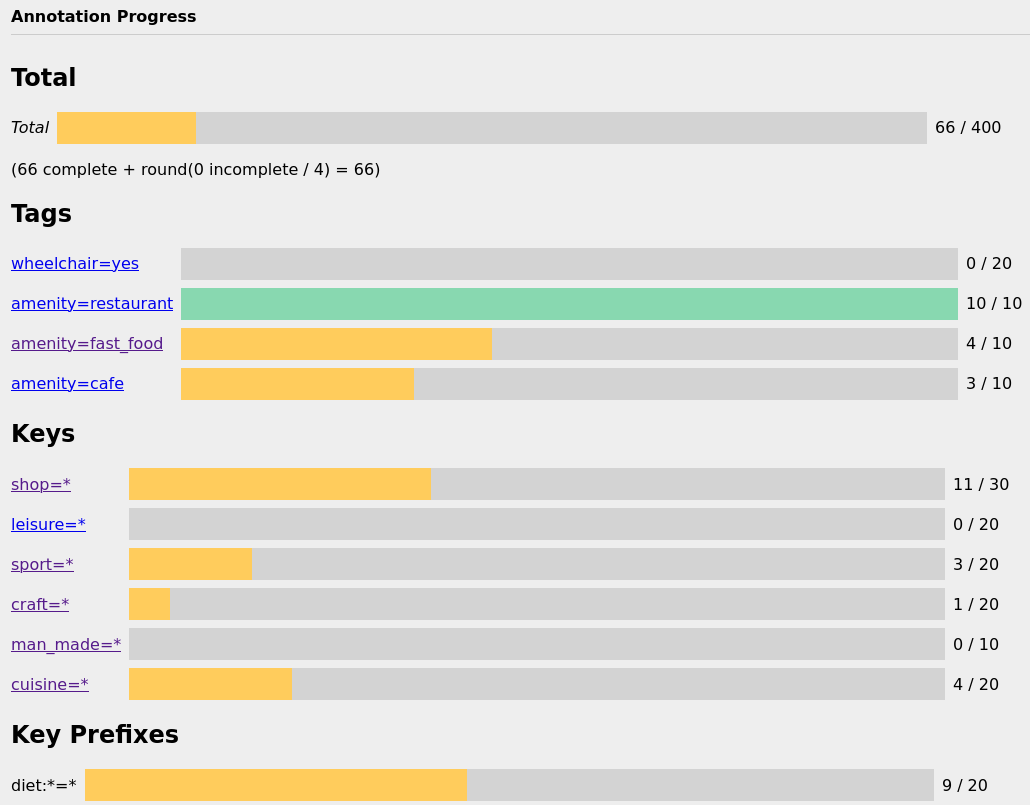
\includegraphics[width=\textwidth]{fig/annotation_progress.png}
  \caption[Annotation progress overview]{Overview of an annotator’s annotation
    progress}
  \label{fig:annotation-progress}
\end{figure}

\section{Online Learning Simulation}
\label{sec:online-simulation}

%%% Local Variables:
%%% coding: utf-8
%%% mode: latex
%%% TeX-engine: xetex
%%% TeX-parse-self: t
%%% TeX-command-extra-options: "-shell-escape"
%%% TeX-master: "../thesis"
%%% End:

%\chapter{Discussion and Future Work}
\label{ch:discussion}

We spent significant work on analyzing the original \nlmapstwo{} dataset and on
fixing any of its shortcomings as well as possible. The insight gained by this
we also used for generating new synthetic queries. By combining the fixed old
data with the new synthetic data into the \nlmapsthree{} dataset the data
available for pre-training an \nlmaps{} model is vastly improved as shown in the
experiments conducted in Section~\ref{sec:pre-training}. This success naturally
calls for continuing this work by generating even more diverse synthetic data,
which can be done by extending the table mapping NL terms to OSM tags or by
designing new templates. New templates could incorporate verb-based questions
like \nl{Where can I eat chinese food?} or take inspiration from the newly
collected queries in \nlmapsfour{}.

The annotation experiment was successful for the most part and we now have a
natural dataset on which new \nlmaps{} models can be evaluated in a more
sensible way than on the flawed and synthetic previous datasets. However, it
must be acknowledged that the MRL queries the annotators produced reintroduce
some inconsistencies in tag usage that were already observed in \nlmapstwo{}.
This is partly due to simple user error (e.g.\ when an annotator does not know
of or does not think of a similar tag for the same thing, like using only
\osmtag{shop=tailor} and forgetting \osmtag{craft=tailor}), but is partly also
rooted in actual vagueness of the NL queries. E.g., what should really be
selected when asking for a place to buy cigarettes? Only tobacco shops or also
cigarette vending machines or even all kinds of places that might sell
cigarettes like supermarkets or kiosks?

Two different approaches for handling this tag inconsistency come to mind: In a
more \enquote{authoritarian} approach, an abstraction layer between OSM and MRL
could be introduced. This could take the form of a table mapping concepts like
\enquote{tailor} or \enquote{buy cigarettes} – which should then appear in the
MRL – to a manually maintained OSM meaning like \mrl{or(shop=tailor,}
\mrl{craft=tailor)} or \mrl{or(shop=tobacco,} \mrl{vending=cigarettes)},
respectively. But maintaining this mapping would amount to a lot of
(semi-)manual work and it would mean losing the advantage of directly using OSM
tags, which most OSM users are somewhat familiar with.

In contrast, the second approach is guided by thr MRL queries’ denotation: When
several users issue queries with some minimum amount of overlap in their result
sets after interpretation, this – perhaps together with a semantic similarity of
the NL queries – can be taken as a sign that the users are actually asking for
the same thing. It is then left for a system to observe which MRL formulation is
the most popular (or – in a recall-focused approach – the most inclusive) and
regard this as the canonical MRL.

However, even the \nlmapsfourraw{} with its inconsistencies is shown in our
simulations to be very usable for improving the parser in an online learning
setting. Not surprisingly, manually removing the inconsistencies as well as
possible yielded even better results. The Adam optimizer is shown to adapt
faster to new examples while Adadelta is better suited to preserve the
performance on the pre-training dataset. It must be noted that we did not
conduct any true online learning experiment where the annotators would have made
their annotations with the model changing over time. Moreover, albeit the online
simulations did improve the accuracy on the new data, they were outperformed
signifcantly by the simple offline batch learning.

Regardless of the learning setup, the main challenge of any \nlmaps{} dataset
remains predicting the correct tag combination while our models make only few
errors in other parts of the MRL. Aside from collecting a lot more training data
to make the tag distribution in the training set less sparse, zero-shot learning
is a direction which could be explored. In one approach, the tag descriptions
from the OSM wiki or even the whole wiki pages could be used as a knowledge
source for learning about the meaning of tags, perhaps in a similar approach as
in CLIP \parencite{radford-2021}.

Part of the reason for the fact that selecting the correct tags poses the main
challenge is that the MRL structure is actually very simple. In fact, it is too
simplistic for representing some queries that OSM could answer. For example, it
is not possible to ask for places whose name (or description or any other tag)
includes a certain substring nor is it possible to query places which are
\emph{not} tagged with a certain tag. And also referring to one’s own
geographical position isn’t possible resulting in the situation that trivial NL
queries like \nl{closest bus stop near me} have no MRL equivalent. These issues
serve as pointers on how to extend the current MRL.

Due to its success in previous work, a character-based model was used for all
work in this thesis, which has the advantages that no NER system is necessary
for recognizing named entities and copying them to the MRL and that new tags can
easily be accommodated without the need to add them to the target vocabulary.
The downside of the character-based model is that it is fairly sensitive to
spelling variations on the NL side. As observed in the experiments, the spelling
\nl{fire station} was correctly mapped to \osmtag{amenity=fire_station}, but the
spelling variation \nl{firestation} led to the model hallucinating the tag
\osmtag{amenity=firestation}. A related problem is that the character-based
model will probably not be able to take advantage of semantic similarity of NL
queries or even single words. The time is ripe for a modern seq-to-seq model
operating on subword units like BPE at least on the NL side with a pointer
mechanism \parencite{see-2017} for copying the location names from NL to MRL. To
leverage semantic similarity between terms and even whole NL queries,
pre-trained language representations should be incorporated in a similar way as
done by \textcite{chen-2020}.

As of now, \nlmaps{} is unfortunately only available in English. However, the
relative simplicity of most NL queries should make it possible to translate them
into other languages in order to create datasets for parsing NL queries in
languages other than English.

%%% local variables:
%%% coding: utf-8
%%% mode: latex
%%% TeX-engine: luatex
%%% TeX-parse-self: t
%%% TeX-command-extra-options: "-shell-escape"
%%% TeX-master: "../thesis"
%%% End:

%\chapter{Conclusion}
\label{ch:conclusion}

In this thesis, we conducted a detailed analysis of the original \nlmapstwo{}
dataset finding several shortcomings, many of which were introduced by a flawed
approach of generating synthetic data. We fixed these shortcomings as well as
possible and extended the dataset by generating a linguistically diverse dataset
using probabilistic templates. Training on the extended dataset greatly improves
accuracy on unseen data, especially by making the resulting parser robust
against new location names.

We built a web interface for issuing NL queries, which can also be used to
correct wrong parses and which is capable of training the parser on the new
feedback in an online fashion. With the help of hired annotators, we created the
first large \nlmaps{} dataset consisting of real user queries. This new dataset
was used to demonstrate the effectiveness of our online learning setup in
various simulations, although traditional offline learning still proved
superior.

In our experiments and discussion, we gained new insight into what the main
challenges of the \nlmaps{} task are and proposed various directions for
subsequent research.

%%% Local Variables:
%%% coding: utf-8
%%% mode: latex
%%% TeX-engine: luatex
%%% TeX-parse-self: t
%%% TeX-command-extra-options: "-shell-escape"
%%% TeX-master: "../thesis"
%%% End:

%\appendix

%\chapter{Acknowledgements}
\label{ch:acknowledgements}

% TODO: Where does the money come from?

I want to thank my supervisor Prof.~Dr.~Stefan Riezler for always being ready to
discuss the state of my work, for providing me with helpful guidance about which
approaches to pursue and for his help in finding relevant related work.
Additionally, I want to thank him for making the annotation experiment possible
by financially enabling it with funds from the Google-supported project
\enquote{Learning to Negotiate Answers in Multi-Pass Semantic Parsing}.

Furthermore, I also want to thank Raphael Schumann and especially Michael
Staniek for valuable comments on the ongoing research in numerous discussion
sessions. Michael also made his parsing model available to me, which was used as
one of the foundations of this thesis. An even more integral foundation is of
course Carolin Lawrence’s pioneering work on NLMaps, without which this thesis
would not exist today.

Finally, I would like to acknowledge the great work of the motivated annotators
from all over the world who participated in my annotation project, including the
OSM mappers Benjámin Zachár, Mateusz Konieczny, Rabin Ojha. Especially Mateusz
and another very experienced mapper (here unnamed) were a great help in
debugging issues with the web interface, in discussing finer points of OSM
tagging questions and by providing valuable hints for how to improve NLMaps in
the future.

%%% Local Variables:
%%% coding: utf-8
%%% mode: latex
%%% TeX-engine: luatex
%%% TeX-parse-self: t
%%% TeX-command-extra-options: "-shell-escape"
%%% TeX-master: "../thesis"
%%% End:

\backmatter

\printbibliography[nottype=online]

\printbibliography[type=online,title={Online Resources}]

\end{document}
%%% Local Variables:
%%% coding: utf-8
%%% mode: latex
%%% TeX-engine: xetex
%%% TeX-parse-self: t
%%% TeX-master: t
%%% TeX-command-extra-options: "-shell-escape"
%%% End: